\documentclass[a4paper,10pt]{report}
\usepackage[margin=1.2in]{geometry}
\usepackage{float}
\usepackage[T1]{fontenc}
\usepackage[utf8]{inputenc}
\usepackage{lmodern}
\usepackage[hidelinks]{hyperref}
\usepackage{graphicx}
\usepackage{tikz}
\usepackage{array}
\usepackage[french,italian]{babel}
\usepackage[most]{tcolorbox}
\usepackage{minted}
\frenchspacing

\setlength{\parindent}{0pt}

\pagenumbering{roman} % comincia a mostrare il numero di pagina

\newcommand{\spacer}[1][8pt]{
    \par\vspace{#1}
}

\newenvironment{sitemize}{%
    \begin{list}{\labelitemi}{%
        \setlength{\itemsep}{0pt}%
        \setlength{\parskip}{0pt}%
        \setlength{\parsep}{0pt}%
        \setlength{\topsep}{0pt}%
        \setlength{\partopsep}{0pt}%
        \setlength{\leftmargin}{1.5em}%
        \setlength{\labelwidth}{1em}%
        \setlength{\labelsep}{0.5em}%
    }%
}{%
    \end{list}%
}

\newtcolorbox{note}{
    enhanced,
    breakable,
    colback=lightgray!20,
    colframe=gray!50,
    borderline west={2pt}{0pt}{gray!80},
    arc=0mm,
    boxrule=0mm,
    boxsep=2mm,
    left=6pt,
    right=6pt,
    fonttitle=\bfseries,
    fontupper=\small\color{black!80}
}

\title{\Huge \textbf{Sistemi Operativi}\\ \large Ingegneria Informatica - Unipd}
\date{}
\author{}

\lstset{basicstyle=\small}

\begin{document}

\maketitle

\tableofcontents

\cleardoublepage

\pagestyle{plain} % comincia a mostrare il numero di pagina
\setcounter{page}{1}
\pagenumbering{arabic}

\part{Introduzione}
\chapter{Architettura di un Elaboratore}

Questo non è il primo capitolo che viene trattato nel corso, tuttavia per mantenere un ordine migliore è importante comprendere il funzionamento dell'hardware in quanto il sistema operativo ci interagisce strettamente.

Parte degli argomenti del capitolo sono già stati studiati durante il corso di Architettura degli Elaboratori vengono poi introdotti i sistemi multiprocessori, la cui gestione occuperà parte significativa del corso.

\section{Central Processing Unit}

Il compito della CPU è quello di \textbf{eseguire i programmi} immagazzinati nella memoria centrale, leggendo le loro istruzioni ed eseguendole in sequenza.

La CPU opera in modo ciclico, ripetendo fino alla fine del programma le operazioni di \textbf{fetch-decode-execute}: acquisisce l'istruzione, la decodifica e la esegue

\begin{figure}[H]
    \centering
    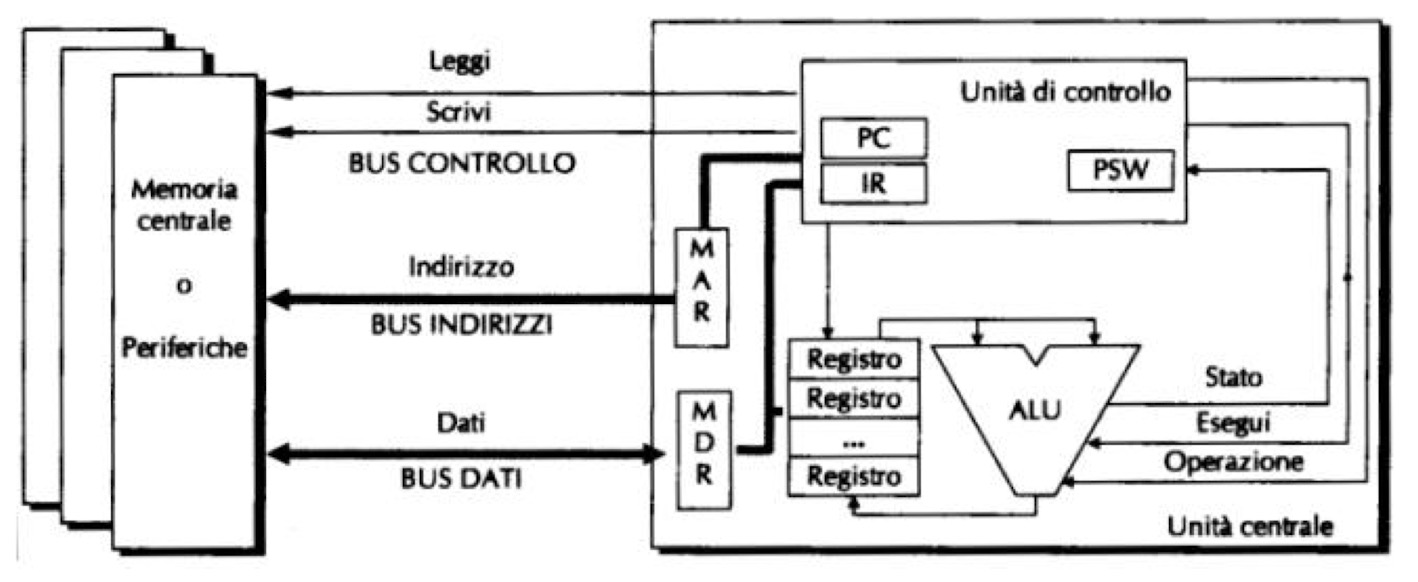
\includegraphics[width=0.55\linewidth]{assets/cpu-architecture.jpg}
\end{figure}

Una CPU è composta da:
\begin{sitemize}
    \item \textbf{Unità di controllo:} ha il compito di leggere le istruzioni e determinarne il tipo.
    \item \textbf{Arithmentic and Logic Unit (ALU):} Esegue le operazoni matematiche necessarie per l'esecuzione dell'istruzione.

    I dati devono partire dai registri e il risultato deve tornare nei registri, questo percorso viene detto \textit{data path}, ogni istruzione comporta l'esecuzione di uno o più cicli di \textit{data path}.
    \item \textbf{Registri:} Una memoria di piccole dimensioni che risiede all'interno del processore, viene utilizzata per memorizzare i risultati temporanei e le informazioni di controllo della CPU.

    \begin{note}
        Due registri particolarmente importanti sono l'Instruction Register (IR) che immagazzina l'istruzione corrente e il Program Counter (PC) che punta alla prossima istruzione.
    \end{note}

    \item \textbf{MDR:} è un registro a cui la ALU ha accesso diretto e che contiene momentaneamente i dati da/per la CPU.
    \item \textbf{MAR:} è un registro della CPU contenente l'indirizzo della locazione di memoria RAM in cui si andrà a leggere o scrivere un dato.
    \item \textbf{Bus di Controllo:} un bus che permette alla CPU di specificare che operazione deve svolgere sulla memoria.
    \item \textbf{PSW:} \textit{Program Status Word} i bit che forniscono informazioni sul risultato dell'ultima operazione eseguita. (overflow, carry, segno)
\end{sitemize}

Ogni ciclo di esecuzione si compone di alcuni passaggi:
\begin{sitemize}
    \item Il valore di PC viene copiato nel MAR
    \item La memoria scrive sul MDR il valore all'indice specificato dal MAR
    \item Il valore di MDR viene copiato sull'IR
    \item L'istruzione viene eseguita dall'ALU
    \begin{sitemize}
        \item Se l'istruzione richiede degli operandi essi devono essere inseriti nei registri attraverso MAR e MDR, similmente a quanto fatto per l'istruzione
    \end{sitemize}
    \item Terminata l'esecuzione il risultato viene scritto sul MDR e l'indirizzo di destinazione sul MAR, la memoria poi si occupa di copiare il valore.
    \item Si ricomincia dal primo punto con l'istruzione successiva.
\end{sitemize}

\section{Prestazioni di un Elaboratore}

Sia un processore con una frequenza di clock $F$ e quindi con periodo di clock $T = \frac{1}{F}$. Questo è il tempo necessario per eseguire un ciclo di \textit{data path}.

\subsubsection*{Istruzioni al secondo}
Per svolgere un'istruzione che richiede $n$ cicli di \textit{data path} $t_{i} = n \cdot T$

Quindi il numero di istruzioni processate al secondo sarà $N = \frac{1}{t_{i}} = \frac{F}{n}$

\subsubsection*{Tempo di esecuzione di un processo}
$$T_{es} = T \cdot (\sum_{i=1}^n N_i \cdot CPI_i )$$

Dove $N_i$ è il numero di istruzioni di tipo $i$ e $CPI_i$ (Cicli Per Istruzione) è il numero di cicli richiesto per l'esecuzione di quel tipo di istruzioni.
(Questo calcolo si applica per una CPU ad un core senza pipeline.)

\subsubsection*{Confronto delle Prestazioni tra due Processori}
Definiamo la prestazione di un sistema come $P = \frac{1}{T_{es}}$.

Il fattore di speedup tra due sistemi, A e B è $\frac{P_A - P_B}{P_B} = \frac{T_B - T_A}{T_A}$

\spacer
La \textit{Legge di Amdahl} ci permette calcolare il miglioramento che si ottiene accelerando di un fattore $a$ un determinato sotto insieme di istruzioni ($p$ è la percentuale di operazioni accelerate).

$$T_{es, finale} = \frac{p \cdot T_{es, iniziale}}{a} + (1-p) \cdot T_{es, iniziale}$$

\subsubsection*{Misurare le Prestazioni di un Processore}
Un'unità di misura sono le \textit{Instruction Per Second}, $IPS = \frac{f}{CPI}$.

Oppure si possono utilizzare i \textit{Mega FLOting point Per Second (MFLOPS)}, una misura che indica quante operazioni di tipo floating point riesce ad eseguire un elaboratore.

\section{Memoria}

L'architettura pensata da Von Neumann richiede una grande quantità di memoria rapida dove salvare tutti i dati dei programmi, questo non è però economicamente possibile.

\spacer
La memoria principale dei sistemi moderni costituita da \textbf{DRAM} (\textit{Dynamic Random Access Memory}) è molto più lenta della CPU limitandone così le prestazioni.

Le memorie con prestazioni comparabili a quelle della CPU sono le \textbf{SRAM} (\textit{Static Random Access Memory}) che sono però troppo costose e quindi possono essere utilizzate solo in quantità limitata.

\spacer
Per questo motivo si costruisce una piramide attorno alla memoria principale, con cache più rapide e piccole al di sopra e dischi lenti, ma estremamente capienti, al di sotto.

\begin{figure}[H]
    \centering
    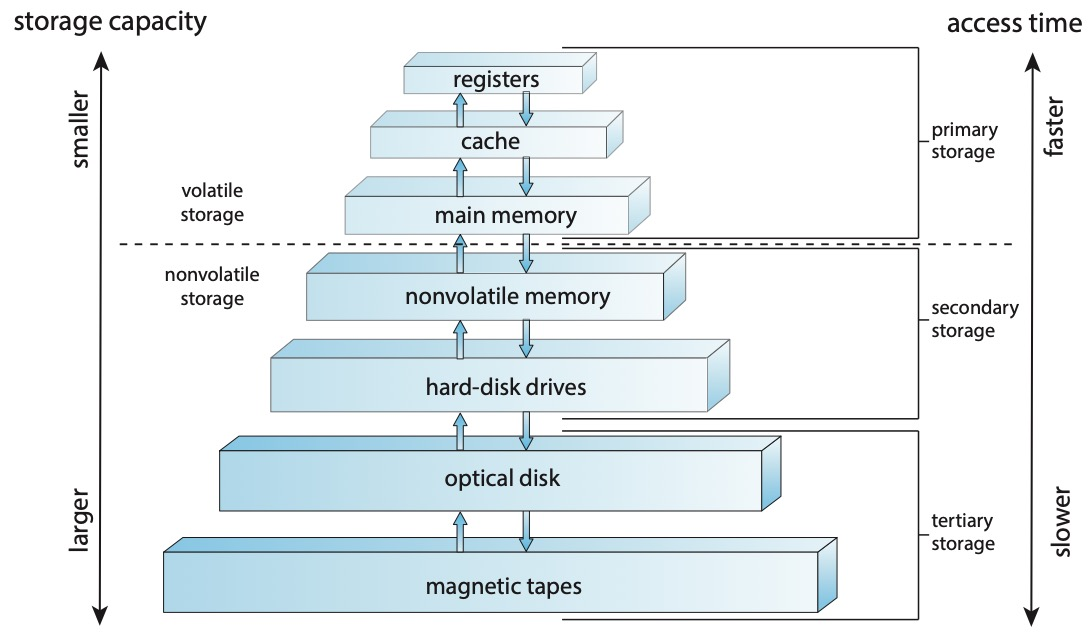
\includegraphics[width=0.48\linewidth]{assets/storage-hierarchy.jpg}
\end{figure}

\subsection{Cache}

La cache si inserisce tra il processore e la memoria principale, quando la CPU richiede un valore esso viene prima cercato nella cache:
\spacer
\begin{sitemize}
    \item \textbf{cache hit:} Il valore viene trovato e può essere restituito alla CPU rapidamente.
    \item \textbf{cache miss:} Il valore non viene trovato, quindi sarà necessario attendere la DRAM.

    Dopo aver recuperato il valore esso, e i valori adiacenti, vengono salvati nella cache, applicando una politica di rimpiazzo se la cache è piena.
\end{sitemize}

\spacer
L'obiettivo è quello di rendere il più grande possibile la percentuale di cache hit sul totale delle richieste.

Per ottenere questo è particolarmente importante sviluppare una \textbf{politica di rimpiazzo} efficace, due principi efficaci a questo scopo:

\spacer
\begin{sitemize}
    \item \textbf{Località spaziale:} È probabile che la CPU debba accedere alle celle adiacenti, come nel caso della lettura di un vettore. È quindi conveniente copiare non solo la cella, ma un intero blocco di memoria RAM.
    \item \textbf{Località temporale:} È più probabile che venga richiesto un dato che è stato chiesto poco prima.
\end{sitemize}

\subsubsection*{Livelli di Cache}
Spesso per ottimizzare i tradeoff della cache essa viene organizzata in livelli (L1, L2, ...) dove più basso è il livello più la cache è piccola e veloce.
Questo viene fatto perché una cache L1 è molto più costosa di una L2 e così via.


Normalmente possiamo dire che la cache di livello $i + 1$ contiene tutti i dati della cache di livello $i$

\begin{note}
    Le prestazioni della cache sono particolarmente importanti per prestazioni dell'intero sistema, se viene progettata in modo corretto può garantire che una percentuale dall'80\% al 99\% degli accessi si limiti ad essa, senza andare alla memoria RAM.
\end{note}

\subsubsection{Esempio}
Una microarchittetura con 3 livelli di cache può essere sturtturata nel seguente modo:

\spacer
\begin{sitemize}
    \item Una cache L1 interna alla CPU, che contiene una parte per le istruzioni, L1-I (16 Kbyte) e una parte per i dati L1-D (64 Kbyte).
    \item Una cache L2, esterna alla CPU, ma contenuta comunque nel package. Di dimensioni maggiori (512 Kb - 1 Mb)
    \item Una cache L3, presente sulla motherboard
\end{sitemize}

\spacer
Le cache L1 e L2, interne al package, hanno un bus riservato, aumentando così le prestazioni.

\begin{figure}[H]
    \centering
    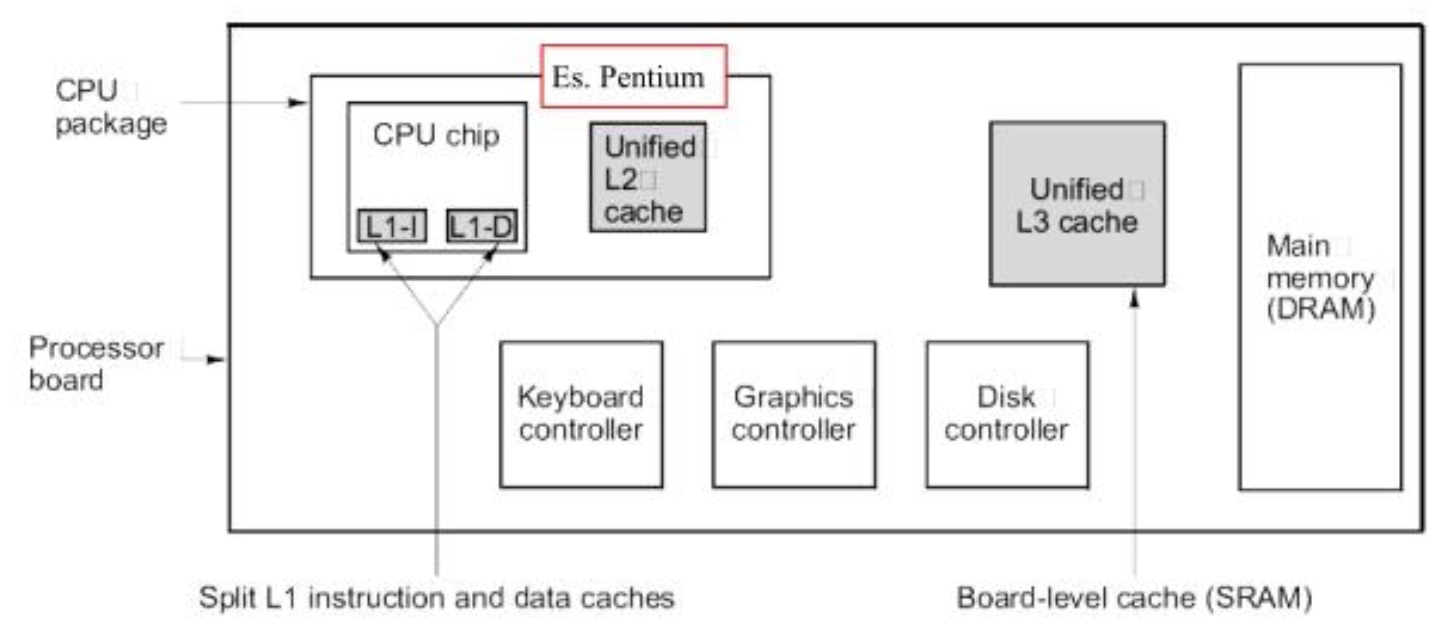
\includegraphics[width=0.5\linewidth]{assets/pentium-cache-architecture.jpeg}
\end{figure}


\section{Parallelismo}
A partire dal 1971 si è sempre rivelata vera la \textit{Legge di Moore} che afferma: "Il numero di transistor per chip, raddoppia ogni 18 mesi".

\spacer
Negli anni i progettisti di processori hanno affrontato con svariate tecniche il problema di tradurre l'aumento di densità dei transistor in un aumento delle prestazioni.

Ogniuna di queste tecniche ha pro e contro:
\spacer
\begin{sitemize}
    \item \textbf{Ridurre il numero di cicli}, quindi migliorare gli algoritmi. Questa è ancora una strada percorribile, ma in 60 anni di ricerca nell'ambito siamo riusciti a trovare soluzioni ottime per i problemi più rilevanti sull'ambito.
    \item \textbf{Aumentare la frequenza di clock} si rivela problematico per l'aumento di calore che viene prodotto, i processori moderni già producono la massima quantità di calore che può essere praticamente dissipata.
    \item Il \textbf{Parallelismo} è la strada che si è intrapresa negli ultimi anni, ha lo svantaggio di richiedere dell'overhead, quindi raddoppiare il numero di core non raddoppia le prestazioni, ma è la strada che permette di sfruttare l'aumento di densità nei transistor.

    Il parallelismo può avvenire al livello dell'istruzione, permettendo più operazioni all'interno dello stesso core (pipeline). Oppure può avvenire a livello di core, inserendo più core.
\end{sitemize}

\spacer
I metodi più utilizzati per realizzare il parallelismo sono:

\spacer
\begin{sitemize}
    \item \textbf{Componenti piccole} che \textbf{interagiscono fortemente tra loro}.

    Con questa soluzione viene parallelizzata la singola operazione (\textit{parallelismo fine-grained})

    Un esempio si trova nell'hyperthreading che permette ad una CPU di eseguire più processi allo stesso tempo.

    \item Un \textbf{piccolo numero di CPU grandi} dotate di \textbf{interconnessioni a bassa velocità}.

    Con questa tecnica l'elemento che viene parallelizzato è l'intero processo  (\textit{parallelismo course-grained})

    Ne sono esempi i sistemi multicore e la realizzazione di chip dedicati a specifiche operazioni.

\end{sitemize}

\begin{figure}[H]
    \centering
    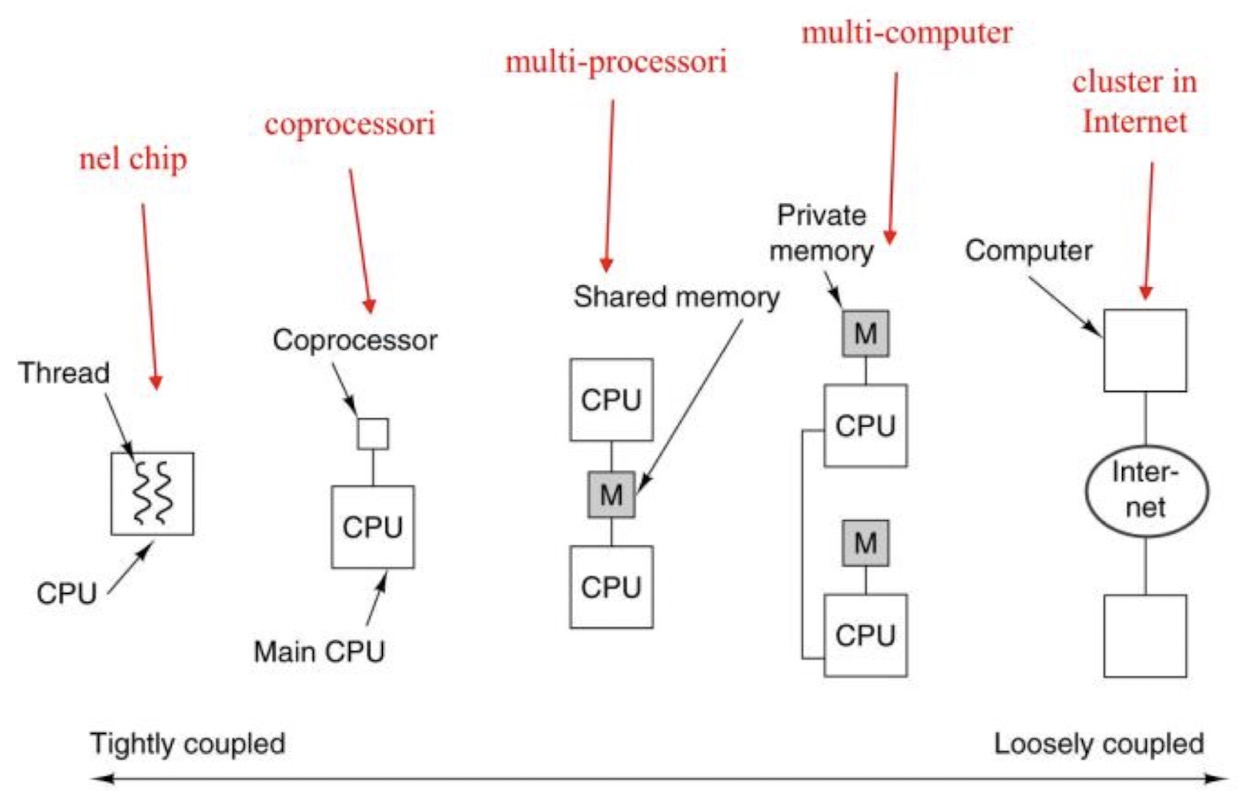
\includegraphics[width=0.45\linewidth]{assets/parallellismo.jpg}
\end{figure}

Gli elementi che caratterizzano il parallelismo, dal punto di vista hardware sono:
\begin{sitemize}
    \item \textbf{Natura e numero degli elementi di calcolo}, pochi elementi a prestazioni elevate, oppure molti elementi a basse prestazioni
    \item \textbf{Natura e numero degli elementi di memoria} La memoria viene divisa in moduli per permetterne l'accesso a tutti gli elementi di calcolo, il modo in cui viene divisa influenza il parallelismo
    \item \textbf{Modalità di connessione} Le connessioni possono essere di tipo statico, oppure dinamico, gestite tramite uno switch in grado di instradare i messaggi.
\end{sitemize}

\subsection{Implementazioni}
Il parallelismo può essere quindi implementato su più livelli:
\begin{sitemize}
    \item \textbf{A livello di istruzioni} tramite pipeline.
    \item \textbf{Multi-threading} Due thread vengono eseguiti contemporaneamente, una CPU virtualizza due CPU.
    \item \textbf{Multi-core} Consente il completo multi-threading di più processi.
    \item \textbf{Core Eterogenei} all'interno dello stesso chip, ognuno con funzionalità specializzate.
\end{sitemize}

\begin{note}
    Sia intel (a partire dall'architettura Ice Lake) che Apple (con i suoi Apple Silicon), implementano un'architettura ibrida, con core ad alte prestazioni e altri core per processi di minore importanza.
\end{note}
\section{Multiprocessori e MultiComputer}
Il modo forse più diretto per implementare il parallelismo è quello di aggiungere più processori, creando un \textbf{multiprocessore}.

Se essi condividono la stessa memoria essi possono essere trattati come un unico processore e sono un esempio di un sistema \textit{strongly coupled}.

\begin{figure}[H]
    \centering
    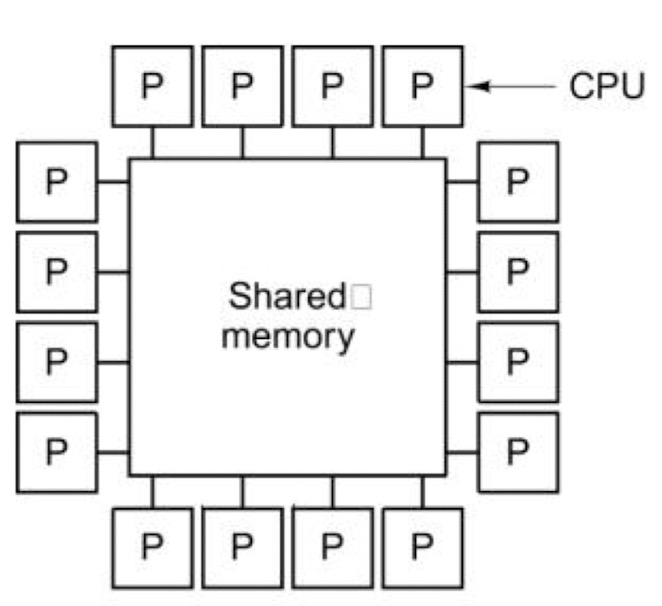
\includegraphics[width=0.28\linewidth]{assets/multiprocessore.jpg}
\end{figure}

Per inserire una potenza di calcolo ancora maggiore è necessario unire due o più multiprocessori in un \textbf{multicomputer}.

In questo caso risulta essere più complessa la programmazione, in quanto i sistemi sono \textit{loosely coupled} ed è necessario tenere conto degli overhead dello scambio di informazioni, ma a livello hardware sono molto più semplici da costruire a parità di core.

\begin{figure}[H]
    \centering
    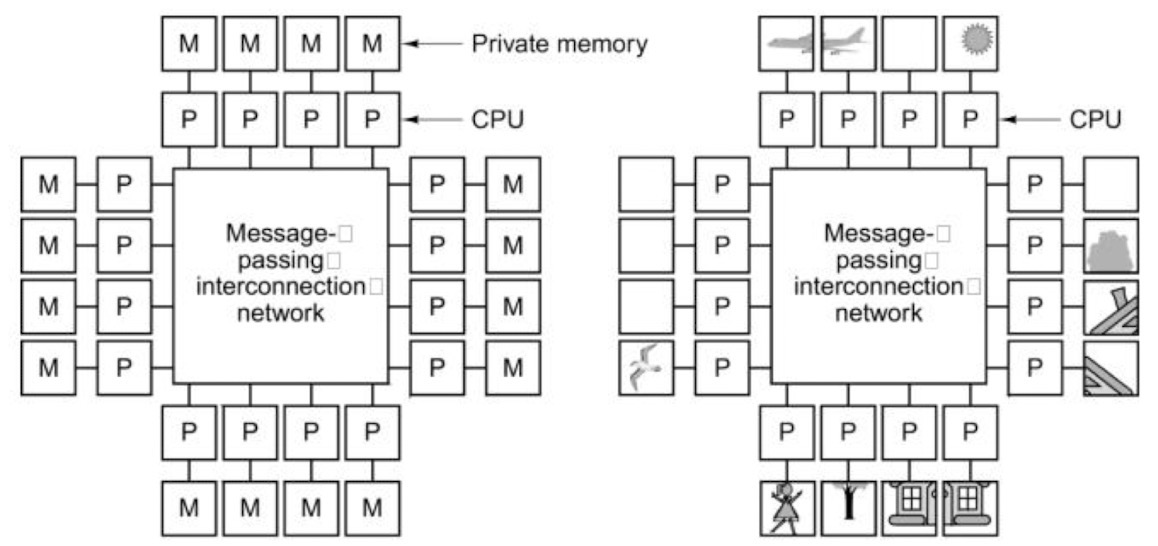
\includegraphics[width=0.62\linewidth]{assets/multicomputer.png}
\end{figure}

\begin{note}
    Quando due SoC sono connessi con una connessione con larghezza di banda sufficiente essi possono essere trattati come un unico chip. Ad esempio la serie Ultra dei chip Apple Silicon ha una connessione "DeepFusion" a 2.5 TB/s a bassa latenza.
\end{note}

\subsection{Topologia delle Connessioni}

In un sistema multicomputer la \textbf{topologia} delle connessioni tra i vari computer diventa di centrale importanza, si cercano le migliori prestazioni riducendo la quantità di connessioni necessarie.

\begin{figure}[H]
    \centering
    \begin{minipage}{0.45\textwidth}
        \subsubsection{Grado o fanout}
        Il numero di connessioni che passano per un nodo, un grado maggiore indica maggiori tolleranze a possibili interruzioni di rete.
    \end{minipage}
    \hfill
    \begin{minipage}{0.45\textwidth}
        \begin{figure}[H]
            \centering
            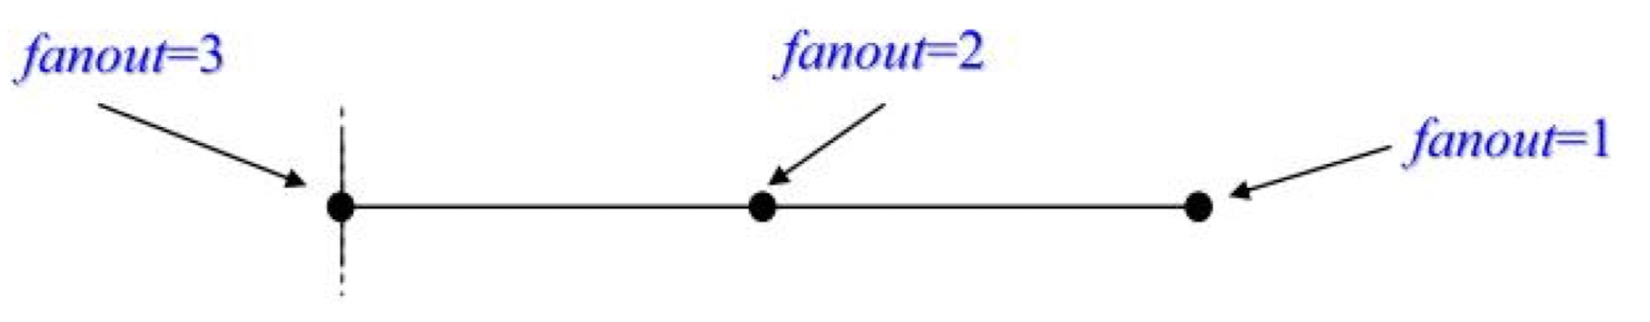
\includegraphics[width=1\linewidth]{assets/fanout.jpg}
        \end{figure}
    \end{minipage}
\end{figure}

\begin{figure}[H]
    \centering
    \begin{minipage}{0.45\textwidth}
        \subsubsection{Diametro}
        Il numero massimo di passaggi tra un nodo e un'altro in una rete, dà informazioni sul tempo di comunicazione nel caso peggiore.
    \end{minipage}
    \hfill
    \begin{minipage}{0.45\textwidth}
        \begin{figure}[H]
            \centering
            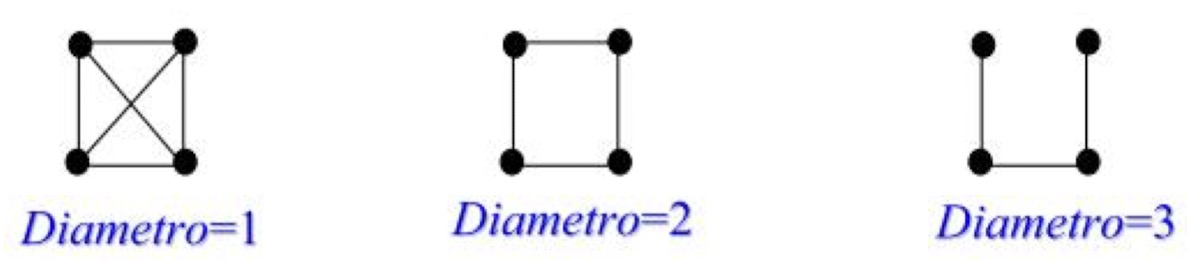
\includegraphics[width=1\linewidth]{assets/diametro.jpg}
        \end{figure}
    \end{minipage}
\end{figure}

\begin{figure}[H]
    \centering
    \begin{minipage}{0.45\textwidth}
        \subsubsection{Dimensionalità}
        Numero di assi che devono essere percorsi per arrivare dal un nodo ad un'altro (caso massimo).
    \end{minipage}
    \hfill
    \begin{minipage}{0.45\textwidth}
        \begin{figure}[H]
            \centering
            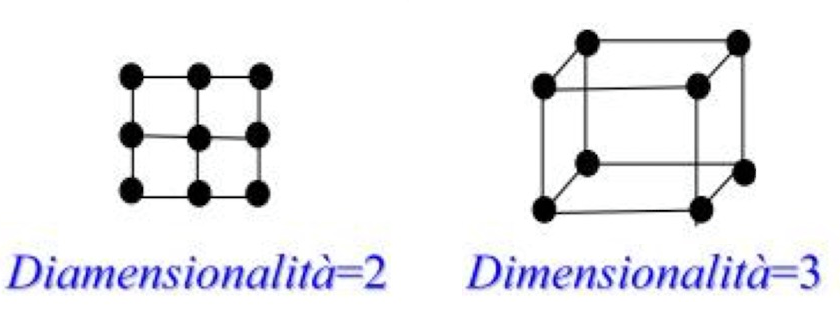
\includegraphics[width=0.65\linewidth]{assets/dimensionalita.png}
        \end{figure}
    \end{minipage}
\end{figure}

\begin{figure}[H]
    \centering
    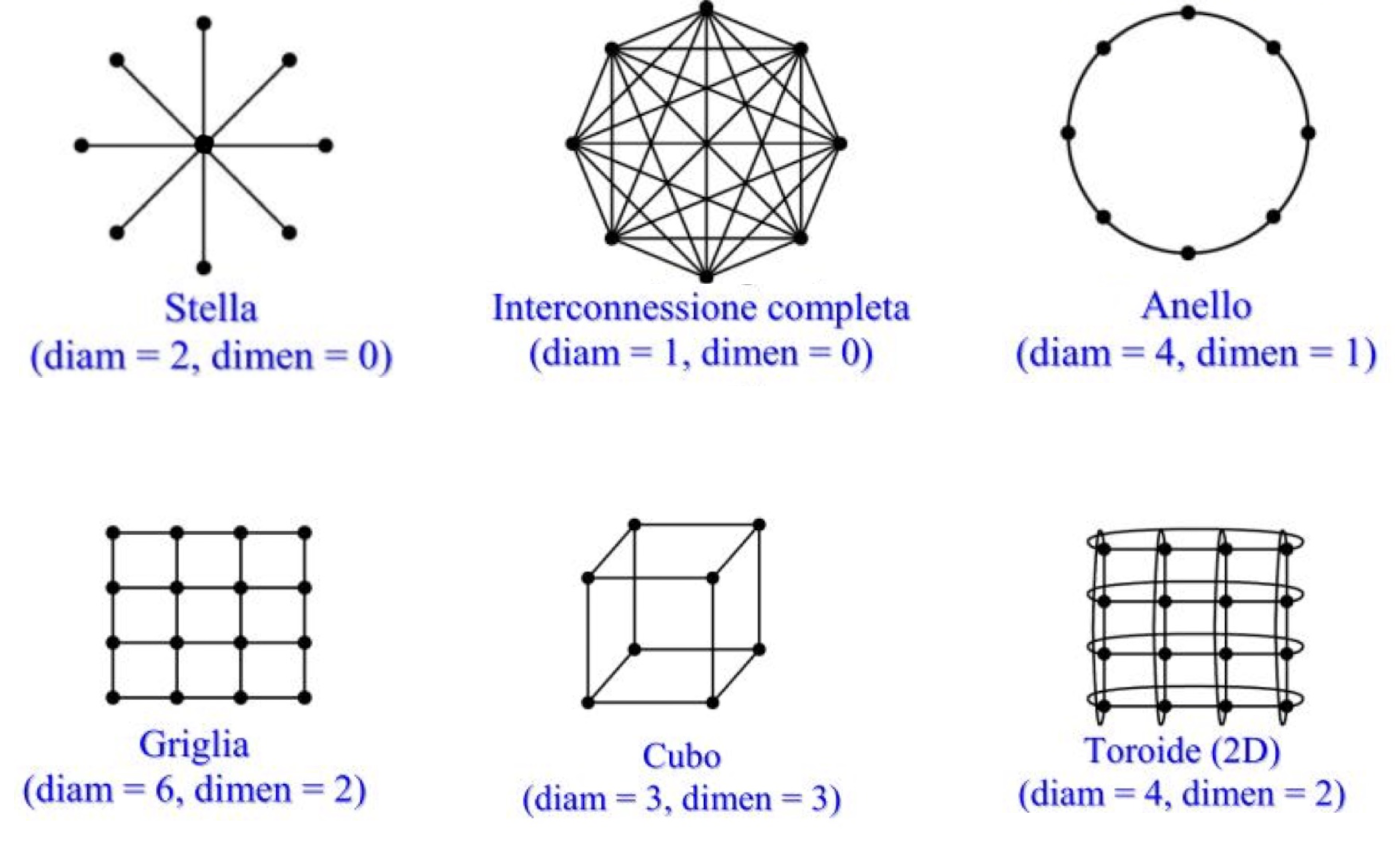
\includegraphics[width=0.5\linewidth]{assets/connessioni.png}
    \caption{Esempi di connessioni}
\end{figure}

\begin{note}
    Nei supercomputer nella maggior parte dei casi si opta per una connessione a toroide 3D, quindi ha dimensione 3, che porta un buon compromesso tra diametro e numero di connessioni.

    \begin{figure}[H]
        \centering
        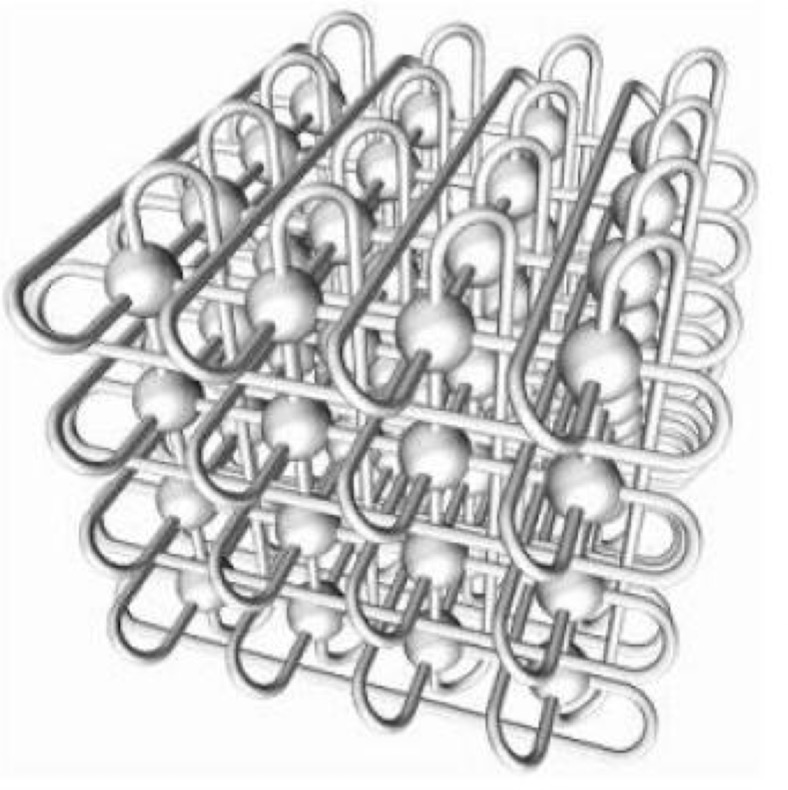
\includegraphics[width=0.3\linewidth]{assets/toroide3d.jpg}
        \caption{Toroide(3D)}
    \end{figure}
\end{note}

\subsection{Prestazioni}
Vogliamo calcolare quanto aumentano le prestazioni se applichiamo $n$ CPU allo stesso problema.

Ovviamente è impossibile ottenere un aumento delle prestazioni pari a $n$.

\spacer
\begin{sitemize}
    \item Esistono parti dei programmi \textbf{intrinsecamente sequenziali}.
    \item La \textbf{comunicazione}, per quanto efficiente, comporta dell'overhead.
    \item Gli \textbf{algoritmi paralleli} sono spesso sub-ottimi rispetto a quelli sequenziali.
\end{sitemize}

$$T_{es, parallelo} = f\cdot T_{es, sequenziale} + \frac{(1-f)\cdot T_{es, sequenziale}}{n}$$

dove $f$ è la frazione di codice sequenziale sul totale.

\subsubsection{Prestazioni e Connessioni}
Aumentare il numero di CPU spesso non è sufficiente per incrementare le prestazioni. È necessario avere un'architettura \textbf{scalabile}.

Delle buone struttura di topologia delle connessioni sono a griglia e a cubo, mentre quella ottimale è l'ipercubo, in quanto il diametro aumenta logaritmicamente rispetto al numero dei processori.

\subsection{Tassonomia o Classificazione dei sistemi}
Quella più utilizzata è quella ideata da Flynn nel 1972 che si basa sulla grandezza delle sequenze di numeri e di dati.

\begin{center}
    \begin{tabular}{ | c | m{2cm} | m{2cm} | c | }
        \hline
        Nome & \raggedright Sequenze di istruzioni & \raggedright Sequenze di dati & Esempi                         \\
        \hline \hline
        SISD & 1                                   & 1                             & Macchina di Von Neumann        \\
        SIMD & 1                                   & Molte                         & Computer Vettoriali            \\
        MISD & Molte                               & 1                             & Solo teoriche                  \\
        MIMD & Molte                               & Molte                         & Multiprocessori, Multicomputer \\
        \hline
    \end{tabular}
\end{center}

\subsection{Implementazioni}

\subsubsection{NUMA}
Spesso il fattore limitante al numero di processori che è possibile aggiungere ad un sistema è la dimensione del bus che porta alla memoria principale.

\spacer
Nell'architettura NUMA si fornisce ad ogni processore una \textbf{memoria locale} a cui può accedere con un suo bus separato.

Inoltre tutti i processori condividono gli stessi indirizzi fisici, quindi la comunicazione tra processori può avvenire facilmente tramite una connessione diretta.

\spacer

Questo rende molto più semplice scalare i sistemi e accelera i tempi di accesso tra il processore e la sua memoria, tuttavia l'accesso alla memoria di un'altro processore è molto rallentato.

\begin{figure}[H]
    \centering
    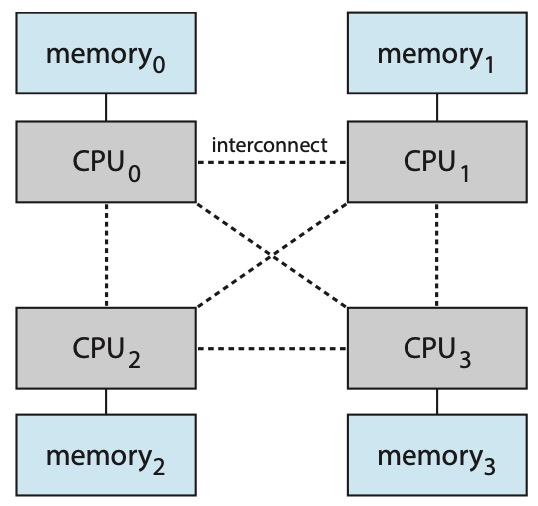
\includegraphics[width=0.3\linewidth]{assets/NUMA.jpg}
    \caption{Visualizzazione sistema NUMA}
\end{figure}

\subsubsection{Cluster}
In modo simile a quanto possiamo fare per più processori possiamo collegare due o più calcolatori completi. I quali possono condividere una memoria secondaria comune.
Questi sistemi sono debolmente accoppiati, quindi non tutte le operazioni possono sfruttare la completa potenza di calcolo.

Anche in questo caso è possibile creare cluster \textbf{asimmetrici} e \textbf{simmetrici}, i primi possiedono un nodo che ha l'unica funzione di gestire gli altri rimanendo in uno stato di attesa attiva, mentre nei secondi tutti i nodi eseguono le applicazioni e si controllano reciprocamente.

\begin{figure}[H]
    \centering
    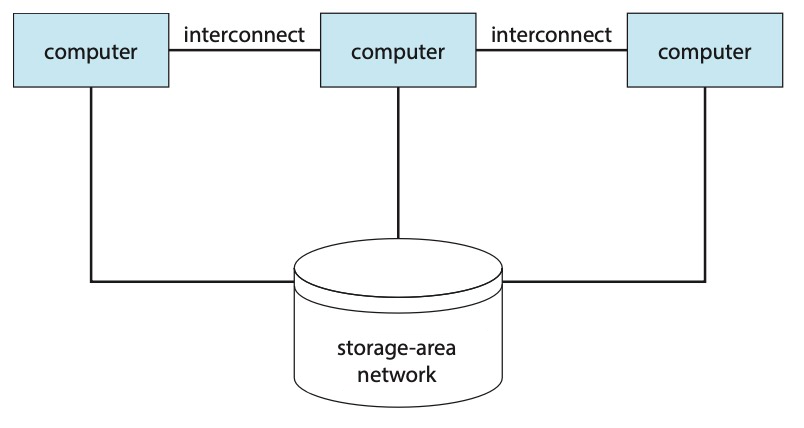
\includegraphics[width=0.5\linewidth]{assets/cluster.png}
    \caption{Cluster}
\end{figure}

\begin{note}
    Questo risulta essere particolarmente utile nel caso di sistemi che devono essere sempre operativi, anche nel caso di un malfunzionamento di uno dei computer il servizio non viene interrotto.

    \spacer
    I Cluster vengono utilizzati anche nell'\textit{High performance computing}, ma le applicazioni devono essere scritte appositamente per poter sfruttare tutte le prestazioni messe a disposizione dal cluster.
\end{note}

\subsection{Coprocessori}
Un coprocessore è un processore \textbf{indipendente} che esegue compiti specializzati sotto il controllo del processore principale.

\spacer
\begin{sitemize}
    \item \textbf{Coprocessori di rete:} Specializzati per gestire ad alta velocità i pacchetti di rete.
    \item \textbf{Crittoprocessori:} Consentono di cifrare/decifrare velocemente flussi di dati.
    \item \textbf{Graphical Processing Unit (GPU):} Consente di processare una gran quantità di dati video e grafica 3D. Una singola GPU può contenere fino a qualche migliaio di core grafici.
    \spacer
    Le GP-GPU, \textit{general purpose GPU} grazie a linguaggi di programmazione quali CUDA e OpenCL possono essere facilmente utilizzate per operazioni floating point, rendendole così di grande importanza nell'high performance computing.
    \spacer
    Per ottenere questo tipo di schede grafiche è stato necessario convertire i core per renderli compatibili alle specifiche IEEE per l'aritmetica a singola e doppia precisione. Inoltre è stato necessario fornire accesso in lettura e scrittura alla memoria principale.
    \item \textbf{Tensor Processing Unit (TPU):} Un coprocessore dedicato alle reti neurali per il \textit{deep learning}.
    \item \textbf{Field Programmable Gate Array (FPGA):} È un dispositivo che permette di implementare algoritmi in hardware, tramite software.

    Presenta una serie di blocchi logici configurabili e sono ideali per lo sviluppo e per dei prototipi rapidi.
\end{sitemize}

\section{High Performance Computing}
Con \textit{High Performance Computing} (\textit{HPC}) si intende l'utilizzo di multiprocessori o cluster per effettuare computazioni concorrenti tale che porti a throughput ed efficienza elevati.

Hardware e Software devono essere strettamente collegati per permettere l'utilizzo massivo della parallelizzazione

\subsection{Parallelismo}
Esistono due tipi principali di parallelismo:
\begin{sitemize}
    \item \textbf{Parallelismo delle task} Quando diverse task possono essere esguiti indipendentemente, in questo caso possonoe essere facilmente allocate su diversi core.
    \item \textbf{Parallelismo dei dati} Quando si può operare indipendentemente su porzioni distinte dei dati, in modo da poter suddividere le porzioni su più core.
\end{sitemize}

\subsection{Utilizzo delle GPU}
Mentre per le CPU l'incapacità di aumentare la frequenza e lo spostamento verso sistemi sempre più parallelizzati ha portato ad una riduzione del miglioramento delle performance, le \textbf{GPU}, nate con l'obiettivo di \textbf{elaborare processi parallelamente} hanno continuato a seguire quanto ipotizzato da Moore.

\spacer
Grazie all'architettura \textit{CUDA} le schede video NVIDIA hanno reso possibile la semplice scrittura di programmi altamente paralleli.

Ad oggi si utilizzano CPU solo quando non si può ottenere una grande parallelizzazione, mentre GPU quando è possibile distribuire il carico su un enorme numero di core relativamente poco potenti.

\spacer
Alcune computazioni possono benificiare da un approccio misto tra CPU e GPU, in questo caso il trasferimento dei dati da una memoria all'altra può causare dei rallentamenti anche importanti.

Per questo è in alcuni casi conveniente utilizzare una \textbf{memoria condivisa} così da eliminare questo overhead.

Un'implementazione della memoria condivisa si vede nei chip Apple Silicon che presentano un'unica pool di memoria da cui CPU e GPU attingono.

\begin{figure}[H]
    \centering
    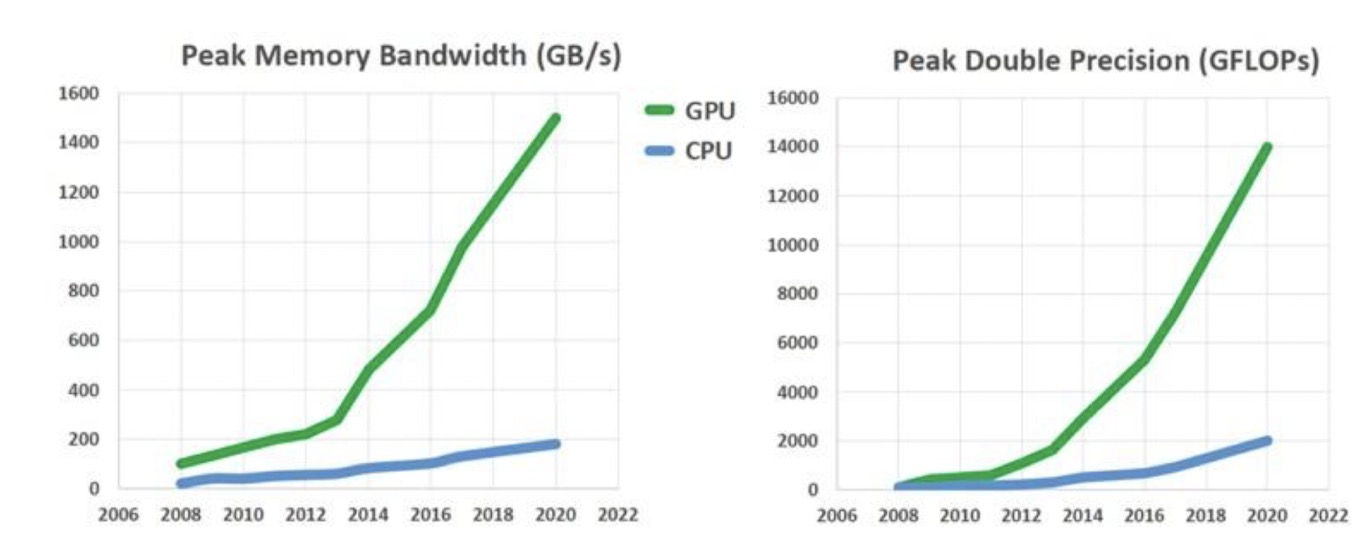
\includegraphics[width=0.65\linewidth]{assets/gflops-gpu-cpu.jpg}
    \caption{Gflops di CPUs e GPUs nel tempo}
\end{figure}

\subsection{TPU}
Da qualche anno Google si è dedicata allo sviluppo di una nuova tipologia di chip chiamati \textit{Tensor Processing Unit}, i quali hanno un set di operazioni ancora più ridotto rispetto alle GPU, ogni core ha quindi una superficie minore, rendendo così possibile stiparne un numero maggiore sullo stesso chip.

\spacer
Questi processori sono indirizzati al \textbf{Machine Learning}, in particolare all'esecuzione di algoritmi per l'allenamento di reti neurali

\subsection{FPGA}

I \textit{Field Programmable Gate Array} sono dei dispositivi che contengono dei blocchi logici configurabili, essi consentono di programmare dell'hardware per fornirgli particolari funzionalità.

\spacer
Essi permettono di implementare funzioni in hardware, con tutti i benfici che questo porta, senza dover sostenere i costi di fabbricazione di un chip.



\chapter{Sistemi Operativi}

Il capitolo punta a fornire delle conoscenze generali sul funzionamento dei sistemi operativi, alcune sezioni verranno poi approfondite successivamente.

\section{Definizione}

Il sistema operativo è quel programma che è \textbf{sempre in esecuzione} quando il computer è acceso, questo viene anche detto il \textit{kernel}, il suo compito è di gestire le interazioni tra l'utente e l'hardware del computer su cui opera.

\spacer
Dato che il sistema operativo si interfaccia direttamente con l'hardware è importante comprendere a fondo la struttura dei moderni computer quali CPU, memoria e dispositivi di I/O. È infatti responsabilità del sistema operativo allocare queste risorse ai programmi.

\spacer
Assieme al \textit{kernel} ci sono altri due tipi di programmi:
\begin{sitemize}
    \item I \textbf{programmi di sistema}, che fanno parte del sistema operativo, ma non sono necessariamente parte del kernel.
    \item Le \textbf{applicazioni}, ovvero tutti i programmi che non sono associati al sistema operativo.
    \item Il \textbf{middleware}, esclusivo ai sistemi operativi per dispositivi mobile, permette di semplificare lo sviluppo delle applicazioni fornendo una collezione di ambienti software per gli sviluppatori.
\end{sitemize}

\begin{figure}[H]
    \centering
    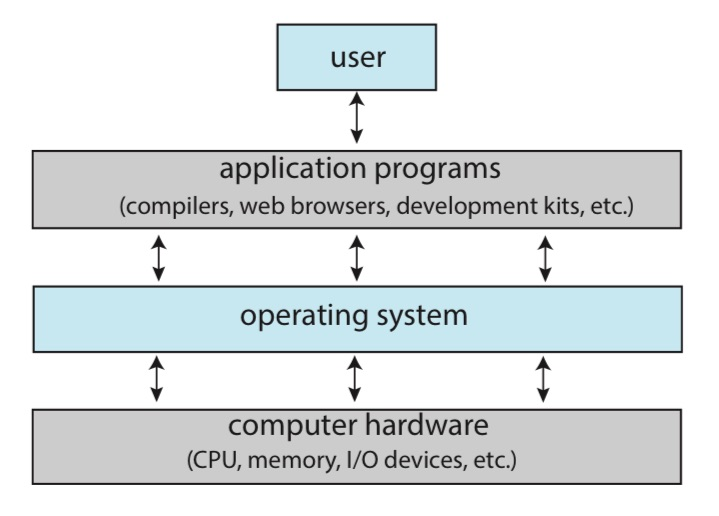
\includegraphics[width=0.45\linewidth]{assets/image.jpeg}
\end{figure}

Il sistema operativo ha diversi compiti rispetto all'utente e all'hardware, questo significa che deve bilanciare prestazioni e semplicità di utilizzo.

\subsubsection*{Lato Utente}
Il sistema operativo deve \textbf{massimizzare le prestazioni} che vengono attribuite a uno o più utenti in modo che esso possa completare il lavoro più velocemente.

\subsubsection*{Lato Hardware}
Dal punto di vista dell'hardware il sistema operativo ha il compito di \textbf{allocare le risorse} ai programmi dell'utente, \textbf{gestire eventuali errori} hardware e software e deve limitare l'utilizzo improprio delle risorse.

\subsection{Modello a Gusci Concentrici}
La struttura del sistema di calcolo può essere schematizzata mediante un "modello a cipolla" o a gusci concentrici.

I gusci circondano l'hardware, ogni livello propone al successivo un'interfaccia di sempre più alto livello, fino ad arrivare all'interfaccia utilizzata dagli utenti.

\begin{figure}[H]
    \centering
    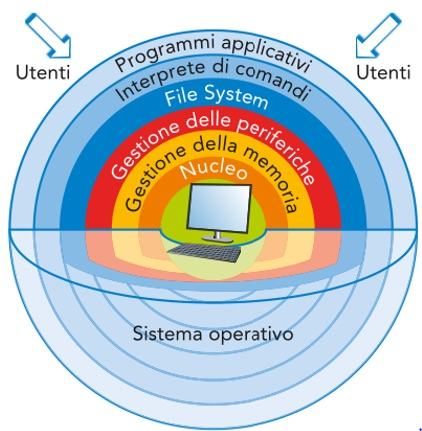
\includegraphics[width=0.35\linewidth]{assets/modello-gusci-concentrici.jpeg}
\end{figure}

\subsection{Avvio}
All'accensione il computer compie una serie di operazioni per arrivare al sistema operativo:

\begin{note}
    \textbf{Legacy BIOS}
    \begin{enumerate}
        \item \textbf{BIOS (\textit{Basic I/O System}):}
              Si trova nella ROM del computer ed è il primo ad essere avvisto.
              esegue check del componenti hardware.
              fornisce una serie di funzioni di base per l'accesso all'hardware
        \item \textbf{MBR(\textit{Master Boot Record}):}
              Il Bios cerca nei dischi un bootloader a cui passare il controllo.
              Questi, se presenti, si trovano nei primi 512 byte del disco, ovvero l'MBR.
        \item \textbf{Boot Loader:}
              Ha al compito di inizializzare il kernel e, di conseguenza, il sistema operativo. Alcuni esempi sono GRUB per linux e BootX per macOS.
    \end{enumerate}
\end{note}

\subsubsection*{UEFI BIOS}
\begin{enumerate}
    \item \textbf{BIOS UEFI (\textit{Unified Extensible firmware Interface})}
    \item \textbf{EFI Boot Loader:}
          Sostituisce MBR e Bootloader, si trova su una partizione del disco di avvio (identificata dalla flag boot)
          Carica Kernel a Sistema operativo
\end{enumerate}

\section{Gestione dell'I/O}
I computer moderni, secondo il modello di Von Neumann, hanno la CPU e i controller hardware connessi direttamente alla memoria principale del sistema.

Per ogni dispositivo hardware esiste un \textbf{controller}. Il sistema operativo ha poi un \textbf{driver} per ogni controller in grado di leggere i dati dal dispositivo e riportarlo in un formato standard.
\begin{figure}[H]
    \centering
    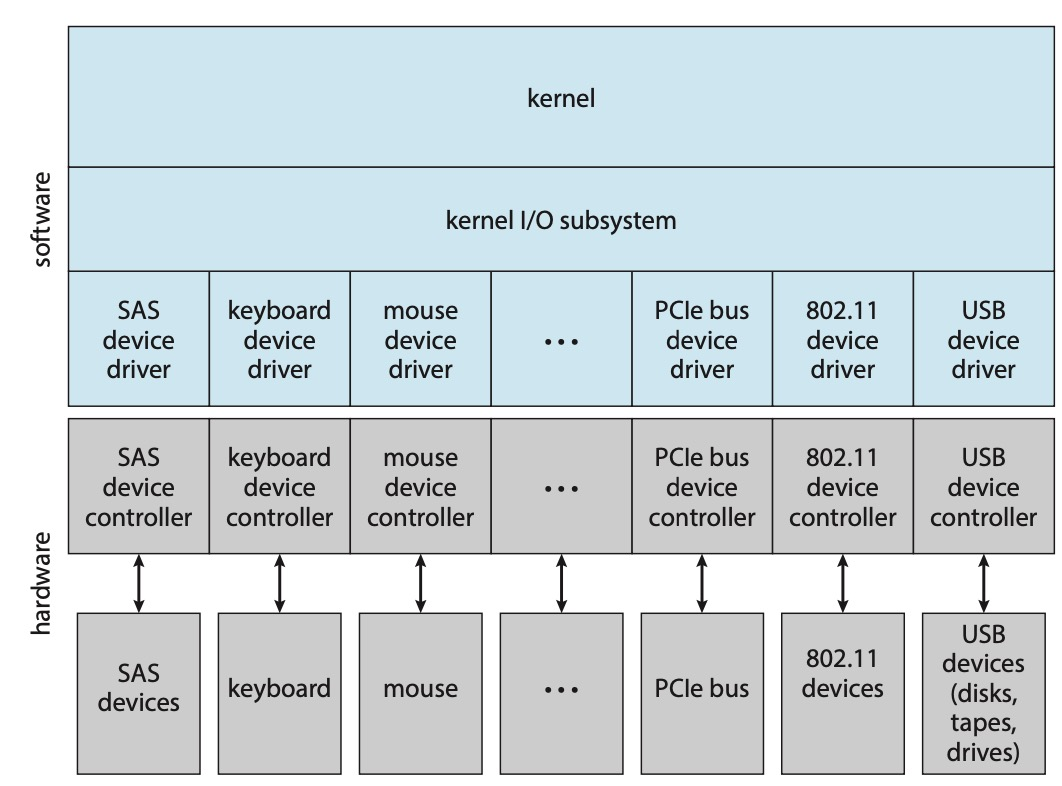
\includegraphics[width=0.45\linewidth]{assets/controller-driver.jpg}
\end{figure}

\begin{note}
    Una cospicua percentuale del codice di un sistema operativo è dedicato alla gestione di I/O, questo per la grande importanza di questi dispositivi rispetto alle prestazioni e l'affidabilità del sistema, inoltre c'è una grande variabilità tra i  vari dispositivi.
\end{note}

\subsection{Interfaccia Comune}
Uno dei compiti del sistema operativo consiste nel nascondere all'utente le caratteristiche dei dispositivi di I/O

Questo viene fatto grazie ad una serie di strategie:
\begin{sitemize}
    \item Il \textbf{Buffering}, ovvero l'uso di un'area di memoria temporanea per immaganizzare dei dati.

    Per esempio la CPU può inserire dei dati in un buffer in attesa che vengano scritti sul disco.
    \item Il \textbf{Caching} consiste nel conservare temporaneamente delle copie dei dati frequentemente utilizzati, anche questa tecnologia viene ampiamente utilizzata nei dispositivi di archiviazione.
    \item Lo \textbf{Spooling} è una tecnica che consiste nell'inserire le richieste di I/O in una coda che viene poi gestita in modo sequenziale.

    Questo consente di gestire più attività contemporaneamente, permette inoltre di continuare l'esecuzione dei programmi del sistema operativo.

    \item Un'\textbf{Interfaccia} generale per i dispositivi.
\end{sitemize}

\subsection{Interrupt}
Un interrupt è il metodo che un dispositivo hardware ha per comunicare con il suo driver.

\spacer
Quando un interrupt si verifica il sistema cerca nel vettore degli interrupt l'indirizzo della subroutine che ha il compito di gestirlo.
Successivamente salva lo stato dell'istruzione interrotta e trasferisce il controllo alla subroutine.

\spacer
Durante la gestione di un interrupt, altri eventuali interrupt giunti al sistema sono momentaneamente “disabilitati”.

\spacer
Gli interrupt sono spesso utilizzati nella gestione dei dispositivi I/O per la loro semplicità, tuttavia quando un dispositivo ha necessità di trasferire grandi quantità di dati l'utilizzo di interrupt può rallentare in modo significativo il sistema.

\begin{figure}[H]
    \centering
    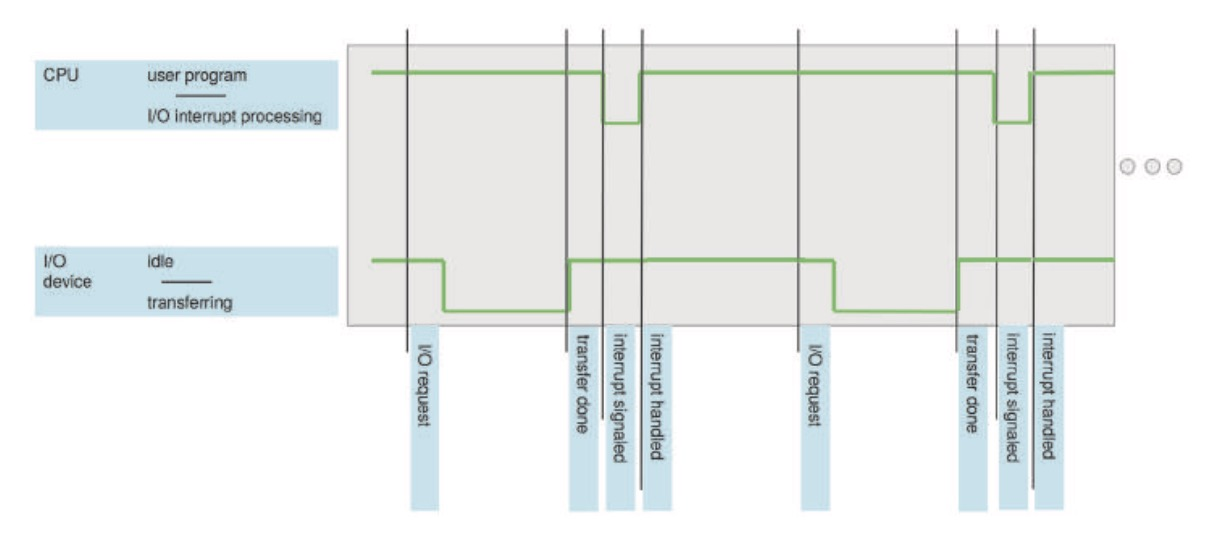
\includegraphics[width=0.65\linewidth]{assets/interrupt-timeline}
    \caption{Timeline per un interrupt}
\end{figure}

\subsubsection{Interrupt sincrono}
È l'implementazione più semplice, dopo la richiesta di dati da parte del sistema esso rimane in idle finché non riceve l'interrupt.

In questo modo viene permessa una sola richiesta alla volta, se ne avvengono due allo stesso istante una delle due dovrà attendere che la gestione del precedente termini.

\subsubsection{Interrupt asincrono}
Dopo la richiesta di dati la CPU continua a svolgere altri processi, controllando periodicamente per l'arrivo dell'interrupt, permettendo così di sprecare meno tempo per ogni operazione I/O.

\begin{figure}[H]
    \centering
    \begin{minipage}{0.4\textwidth}
        \centering
        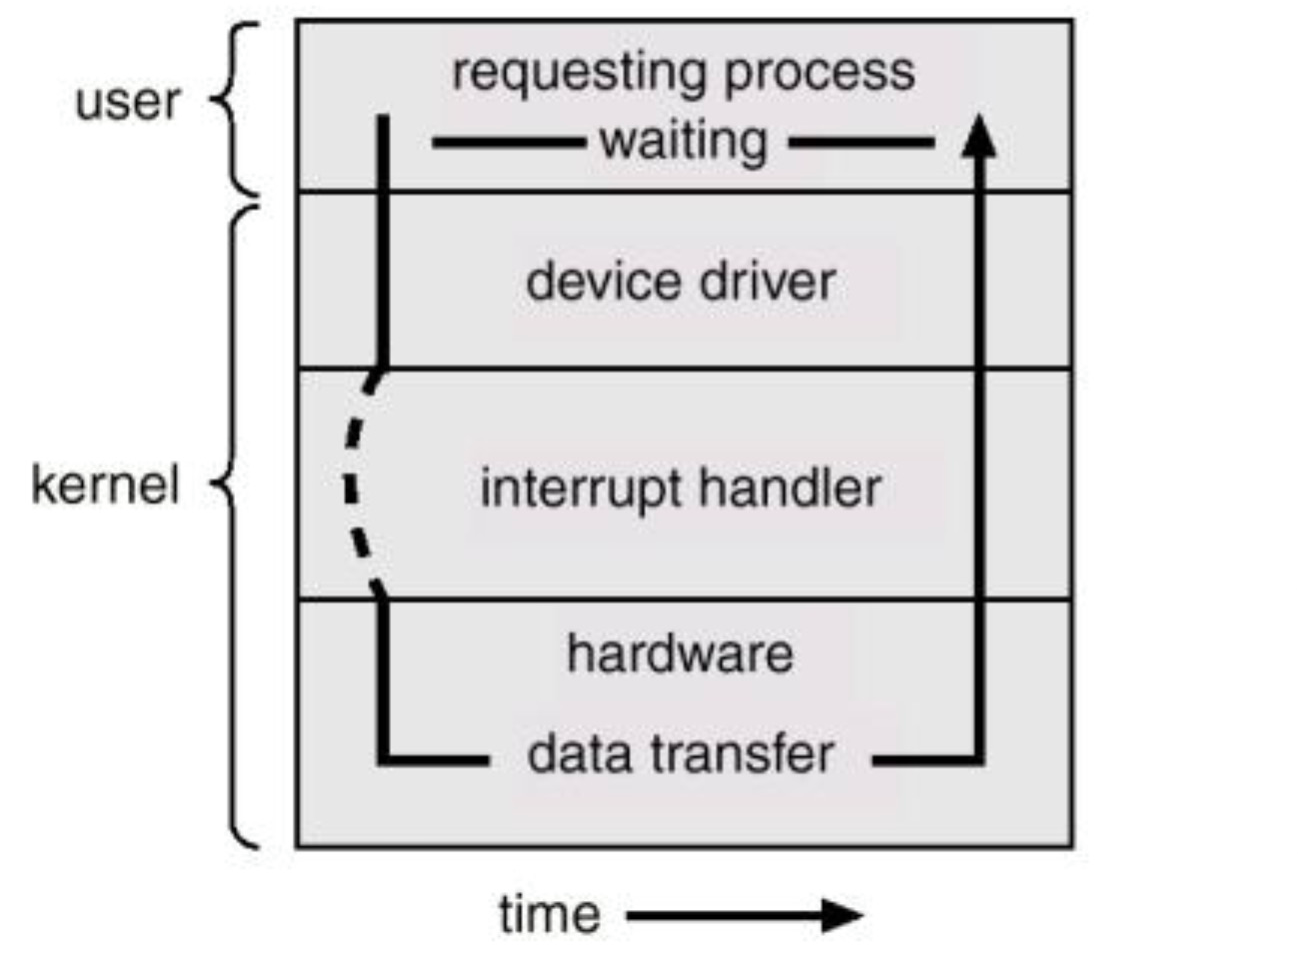
\includegraphics[width=0.8\linewidth]{assets/interrupt-sync.png}
        \caption{Interrupt Sincrono}
    \end{minipage}
    \hspace{0.01\textwidth}
    \begin{minipage}{0.4\textwidth}
        \centering
        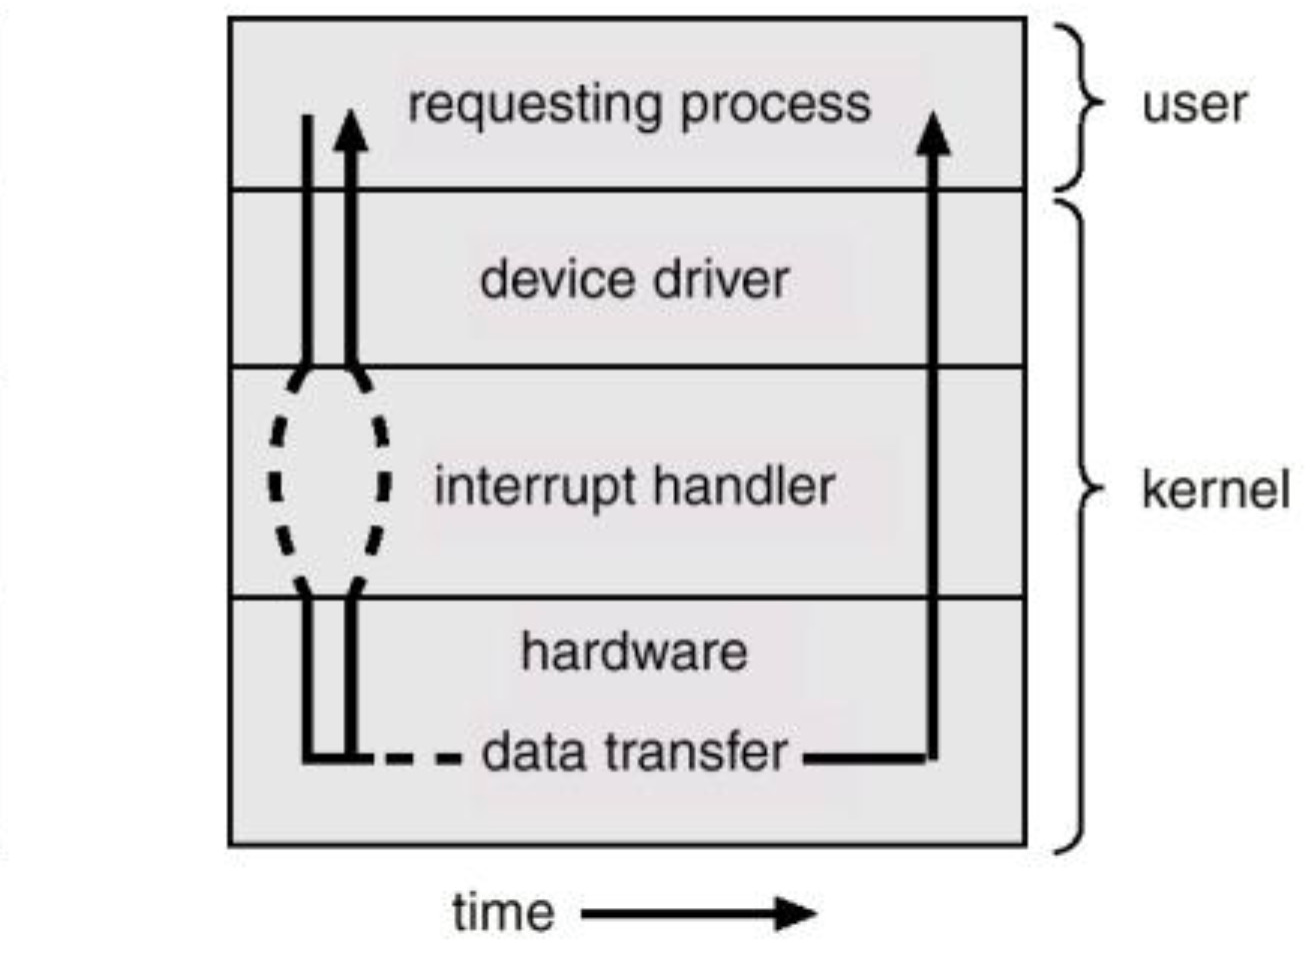
\includegraphics[width=0.8\linewidth]{assets/interrupt-async.png}
        \caption{Interrupt Asincrono}
    \end{minipage}
\end{figure}

\subsubsection{Trap}
Una trap (o eccezione) è un interrupt generato via software, causato da un errore o da una richieste utente (\textit{System Call}).

Le \textit{system call} sono dei meccanismi che possono essere usati da un processo a livello utente o livello applicativo, per richiedere un servizio a livello kernel.


\subsection{DMA}
Il DMA (\textit{Direct Memory Access}) è una strategia che permette di \textbf{trasferire rapidamente grandi quantità di dati}.

\spacer
Dopo che il controller si accorda col il sistema rispetto a dove devono essere scritti i dati in memoria principale, il controller può trasferire interi blocchi di dati senza alcun intervento da parte della CPU.

Viene solo generato un interrupt per ogni blocco trasferito per comunicare che l'operazione è avvenuta con successo.

Utilizzando questa strateglia la CPU è libera di svolgere altre operazioni mentre il controller trasferisce i dati.

\begin{figure}[H]
    \centering
    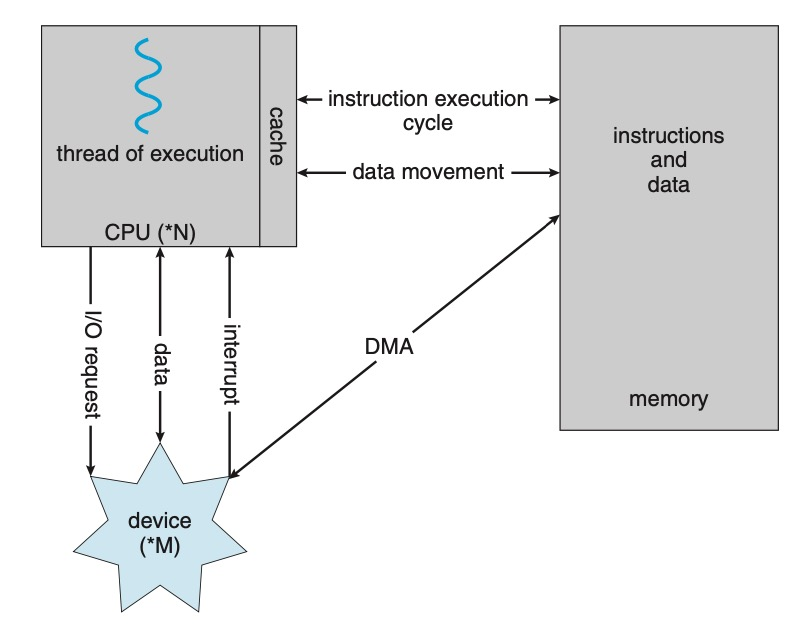
\includegraphics[width=0.45\linewidth]{assets/DMA.jpg}
\end{figure}

\begin{note}
    Esiste anche Remote Direct Memory Access che consente di trasferire dati tra la memoria di due computer, senza sovraccaricare il sistema ricevente.

    Il RDMA è particolarmente utile, se non indispensabile, per processi eseguiti in parallelo tra computer ad alte prestazioni.
\end{note}

\subsection{Operazioni Multimodali}
Proprio come l'hardware anche l'esecuzione del sistema operativo è scandita dagli interrupt. Nel sistema operativo gli interrupt cambiano la modalità di esecuzione dell'hardware.

Tutti i sistemi operativi utilizzano almeno 2 modalità di operazione:
\spacer
\begin{sitemize}
    \item \textbf{User mode:} Modalità dove vengono eseguiti i processi dell'utente, questi processi non hanno completa libertà sul sistema, alcune operazioni sono illegali a questo livello. Se vengono eseguite l'hardware ritorna il controllo al sistema operativo.

    Inoltre anche l'accesso alla memoria ed a altre risorse viene limitato in questa modalità.

    \item \textbf{Kernel mode:} Modalità privilegiata che permette l'accesso completo all'hardware e che viene utilizzata solo dal sistema operativo
\end{sitemize}

\begin{figure}[H]
    \centering
    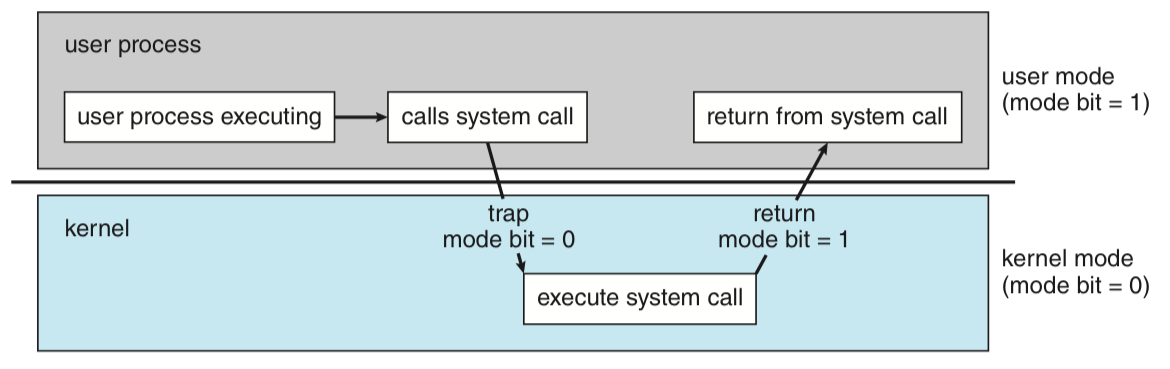
\includegraphics[width=0.65\linewidth]{assets/multimode.png}
\end{figure}

Nelle implementazioni reali vengono utilizzare molte più di 2 modalità, uno tra questi è spesso per le macchine virtuali, mentre altri vengono utilizzati per implementare i livelli di privilegio.

\subsubsection{Timer}
Per prevenire che alcuni processi eseguano cicli infiniti o che semplicemente non restituiscano il controllo al Sistema Operativo gli si fornisce un limite di tempo sull'esecuzione.

Alla creazione di un processo utente si crea anche un timer che se arriva a zero genera un interrupt che ritorna automaticamente il controllo al sistema.

\section{Gestione delle Risorse}

Come visto precedentemente uno dei compiti più importanti del sistema operativo è la gestione delle risorse di sistema, come la memoria, i dispositivi I/O, ecc..

\subsection{Gestione dei Processi}
Un programma è un'entità "passiva", memorizzata sul disco, mentre il processo è "attivo".
I programmi dientano processi quando vengono caricati in memoria principale.

\subsubsection*{Stato del processo}
\begin{itemize}
    \item \textbf{New:} il processo viene creato, diventerà ready appena il sistema operativo lo inserirà nella ready queue.
    \item \textbf{Ready:} il processo risiede in memoria principale ed è in attesa di essere assegnato ad un processore.
    \item \textbf{Running:} Vengno eseguite le istruzioni del processo, i processi vengono selezionati dal dispatcher tra quelli nella ready queue e ci possono ritornano nel caso in cui lo scheduler trovi un processo più importante oppure per un interrupt esterno.
    \item \textbf{Waiting:} il processo è in attesa di un evento, questo avviene da parte del processo stesso nel caso di una richiesta ad un dispositivo I/O
    \item \textbf{Terminated:} il processo ha terminato la propria esecuzione. Può essere dovuto dal processo che ha terminato (o ricevuto un errore), oppure può essere dettato dal sistema operativo per un utilizzo scorretto delle risorse.
\end{itemize}

\begin{figure}[H]
    \centering
    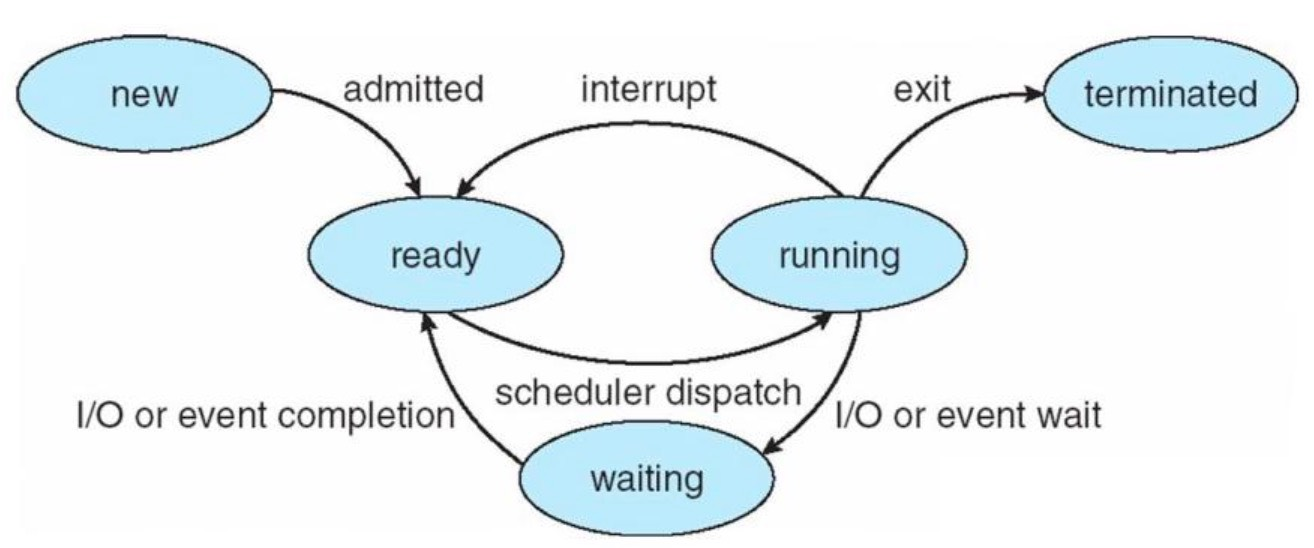
\includegraphics[width=0.6\linewidth]{assets/process.jpg}
    \caption{Process lifecycle}
\end{figure}

\subsubsection*{Informazioni del processo}
\begin{sitemize}
    \item \textbf{Informazioni sul processo} quali stato, priorità e numero identificativo.
    \item Una \textbf{sezione di testo} dove è contenuto il codice del programma da
    eseguire.
    \item Il \textbf{program counter}, l'indirizzo di memoria della prossima istruzione da eseguire ed il \textbf{contenuto dei registri} della CPU.
    \item Lo \textbf{stack}, ovvero i dati temporanei, parametri per i sottoprogrammi, indirizzi di rientro e variabili locali.
    \item Una \textbf{sezione dati}, le variabili globali.
    \item Un \textbf{heap}, memoria dinamicamente allocata durante l'esecuzione del task.
    \item Informazioni sulla \textbf{contabilizzazione} delle risorse (tempo di utilizzo della CPU, ecc... ).
\end{sitemize}

\spacer
Queste informazioni, o i riferimenti a tali informazioni vengono salvati nel \textit{Process Control Block} (PCB), che a sua volta è salvata nella tabella dei processi.

\begin{note}
    Un programma non ha necessariamente un solo processo, ma esso descrive un insieme di processi.
\end{note}

\subsubsection{Threads}
Un processo deve sempre avere almeno un thread (sè stesso), ma può generarne altri in caso abbia bisogno di eseguire delle operazioni simultaneamente sfruttando il multithreading.

\spacer
Tutti i thread di un processo condividono le risorse che sono state assegnate al processo, risiedono nello stesso spazio di indirizzamento e hanno accesso agli stessi dati.

Ogni thread ha un program counter, uno stato, uno spazio di memoria, uno stack e un descrittore.

\spacer
Un processore dotato di Hyper-Threading può eseguire 2 thread contemporaneamente, è in grado di eseguire più istruzioni su dati separati in parallelo.

\subsubsection{Multiprogrammazione e Multitasking}
La multiprogrammazione è un aspetto fondamentale di un sistema operativo. Infatti un singolo processo non è in grado di mantenere sempre occupata la CPU, inoltre spesso gli utenti vogliono essere in grado di eseguire più programmi contemporaneamente.

\spacer
Il sistema memorizza più processi nella memoria principale rendendo possibile così lo switching tra un contesto ed un'altro. Uno specifico algoritmo di scheduling ha il compito di decidere quando e come effettuare questo switch.

\spacer
La multiprogrammazione rende possibile il multitasking, dove il sistema cambia velocemente da un processo all'altro al punto che all'utente sembra che non ci siano interruzioni.

\subsection{Gestione della Memoria}
La memoria centrale ha un'importanza centrale nell'architettura di Von Neumann ed è l'unica memoria di grandi dimensioni a cui la CPU ha accesso diretto (accedere al disco richiede un'operazione di I/O)

\spacer
Il Sistema operativo, rispetto alla memoria principale, ha il compito di:
\begin{sitemize}
    \item Tener traccia di quali parti sono utilizzate e da chi.
    \item Decidere quali processi caricare in memoria quando c'è dello spazio disponibile.
    \item Allocare e deallocare spazio di memoria secondo necessità.
\end{sitemize}

\spacer
Il sistema operativo è anche responsabile di gestire in modo efficiente la memoria secondaria, in quanto spesso non è possibile caricare l'intero programma in memoria principale

\begin{figure}[H]
    \centering
    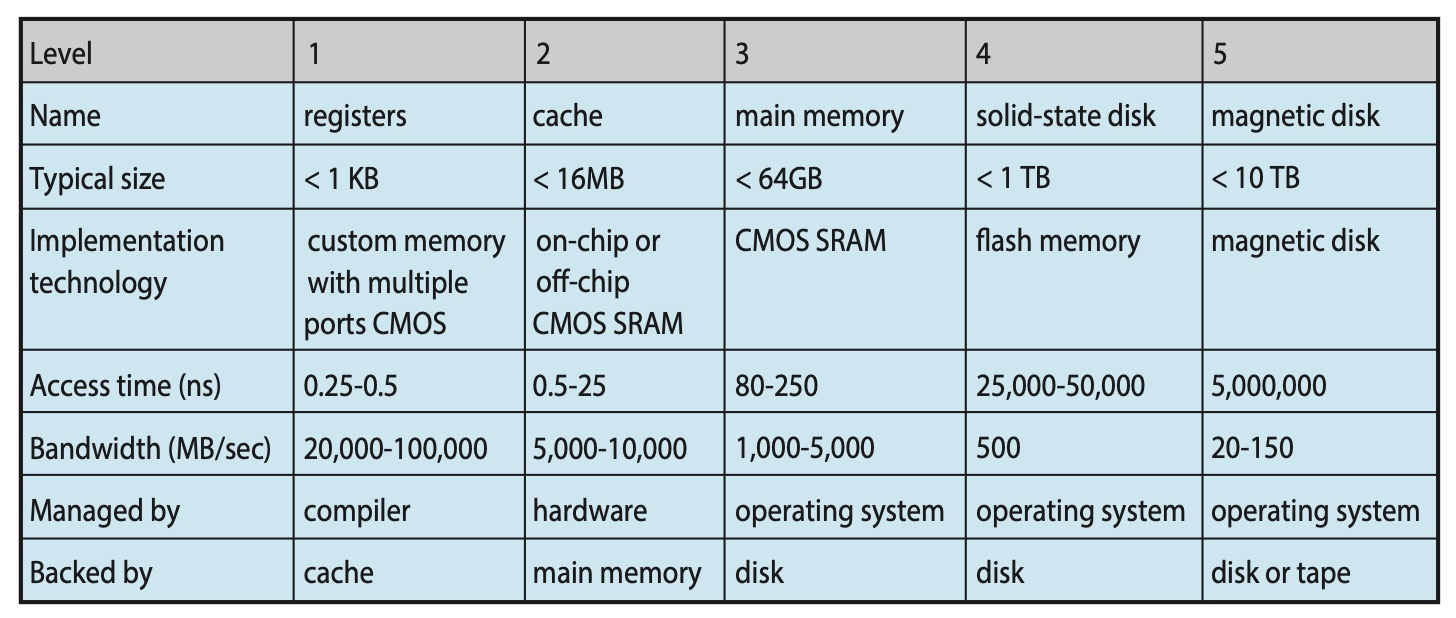
\includegraphics[width=0.75\linewidth]{assets/memory-size.jpg}
\end{figure}

\begin{note}
    Inoltre bisogna considerare che, sopratutto nei sistemi multiprocessore, l'aggiornamento di un dato deve essere riflesso non solo nel file in cui risiede, ma anche in memoria principale e nelle cache degli altri dispositivi.
\end{note}

\subsubsection{File System}
Un file è una \textbf{collezione di informazioni} correlate contenenti dati e programmi.

I file vengono organizzati dal file system in directory, questo permette di effettuare controlli di accesso per verificare che l'utente abbia accesso a quelle risorse.

\spacer
Il sitema operativo è responsabile delle seguenti attività per la gestione di file:
\begin{sitemize}
    \item Creazione e cancellazione di file e directory
    \item Supporto alle funzioni elementari per la manipolazione di file e directory
    \item Associazione dei file ai dispositivi di memoria secondaria
    \item Backup di file su dispositivi stabili di memorizzazione
\end{sitemize}

\subsection{Strutture Dati del Kernel}
Un argomento centrale all'implementazione di un sistema operativo sono le strutture dati, qui vengono descritte le strutture dati utili per la costruzione di sistemi operativi.
Le strutture dati vengono qui solo citate in quanto sono state già approfondite nel corso di Dati e Algoritmi.

\subsubsection{Liste, Pile e Code}
La struttura dati più comune per implementare le liste sono le liste concatenate (standard, doppiamente concatenate e circolari).

Le liste vengono spesso utilizzate per implementare Pile (implementate con politica LIFO) e Code (con politica FIFO).
In particolare la Pila viene utilizzata per implementare lo Stack, utilizzato in diverse situazioni nel sistema operativo.

\subsubsection{Alberi}
Sono utilizzati per rappresentare la relazione causale padre-figlio oppure per implementare degli algoritmi di ricerca binaria efficienti.

\subsubsection{Hashtable}
Vengono utilizzate per memorizzare insiemi di dati con la possibilità di reperire un qualsiasi elemento con una complessità in tempo pari (o quasi) a $O(1)$

\spacer
Le funzioni di hashing banali soffrono del problema del "paradosso del compleanno".
Ovvero in un gruppo di 23 persone la probabilità che 2 di esse compia gli anni lo stesso giorno è >50\%, questo significa che se su una tabella di 365 elementi si inseriscono più di 23 elementi allora c'è una probabilità >50\% di una collisione.

\section{Virtualizzazione}
Una teconologia che permette di \textbf{astrarre l'hardware} di un computer e creare diversi ambienti di esecuzioni. Rende quindi possibile eseguire un sistema operativo come applicazione all'interno di un altro sistema.

\spacer
L'utilizzo di una macchina virtuale garantisce la completa \textbf{protezione delle risorse}, sia per la macchina virtuale che per il sistema ospitante.

La condivisione delle risorse rimane possibile, rendendo possibile la creazione di sistemi estramemente efficienti, dove le risorse di una VM in idle vengono sfruttate dalle altre.

\spacer
Dal punto di vista implementativo la macchina virtuale realizza un'\textbf{interfaccia} indistinguibile da quella di un sistema dedicato.
Le risorse del computer fisico vengono condivise dall'hypervisor o VMM (Virtual Machine Manager) che può sfruttare tutte le funzioni del sistema ospitante per creare l'illusione che ogni utente abbia il proprio sistema.


\subsubsection*{Emulazione}
Un altro aspetto della virtualizzazione è l'emulazione, ovvero la \textbf{simulazione di componenti} hardware in software.

Più in generale è possibile emulare un intero sistema operativo scritto per un'architettura diversa.

L'emulazione però viene ad un costo importante dal punto di vista delle prestazioni, non ci si può aspettare che il codice abbia le stesse performance su tutte le architetture.

\begin{figure}[H]
    \centering
    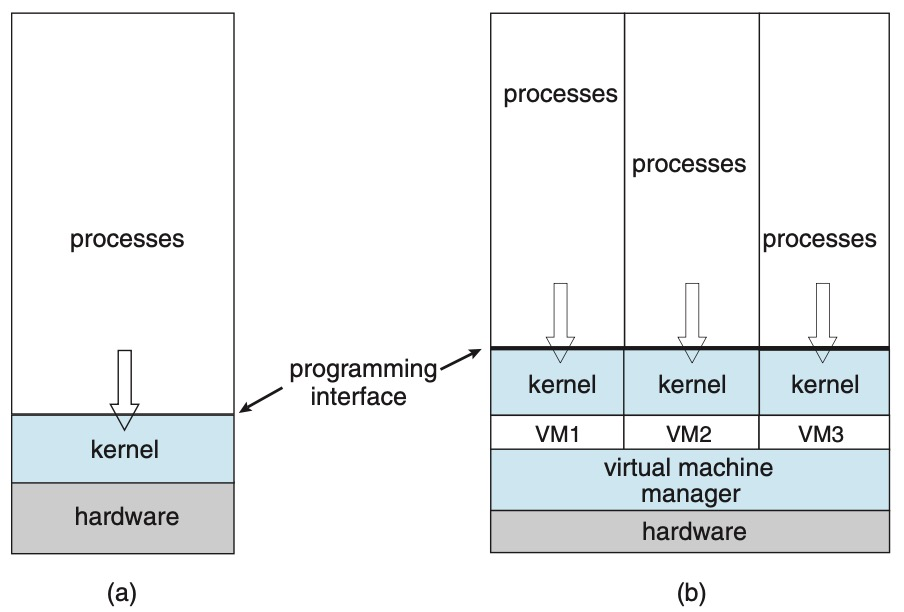
\includegraphics[width=0.4\linewidth]{assets/VMM.jpg}
    \caption{Virtual Machine Manager}
\end{figure}

\begin{note}
    \textbf{Nota di Ingegneria del Software}

    Un' applicazione delle macchine virtuali si trova proprio nello sviluppo e nel test di applicazioni, con una macchina virtuale è possibile testare l'applicazione su varie combinazioni di hardware e software.
\end{note}

\subsubsection*{Apple}
Negli ultimi anni Apple ha costruito diversi strumenti per l'emulazione, a partire dal software Rosetta 2, utilizzato per agevolare la transizione tra mac con processori intel a mac con architettura ARM.
A partire da macOS Sonoma apple ha introdotto il Game Porting Toolkit, uno strumento che permette agli sviluppatori di traddurre giochi scritti in DirectX12 a Metal 3, aumentando notevolemente le prestazioni con un minimo sforzo.

\section{Sicurezza e Protezione}
Nel caso in cui più utenti devono usufruire dello stesso elaboratore l'accesso alle risorse deve essere limitato da regole imposte dal sistema operativo.

È compito delle strategie di protezione quello di fornire le specifiche dei controlli da attuare e gli strumenti per la loro applicazione.

\spacer
La sicurezza comprende tutti i meccanismi di difesa per proteggersi da attacchi interni ed esterni.

Alcuni tipi di attacco possono essere:
\begin{itemize}
    \item \textbf{Denial of Service (DoS o DDoS):} L'attacco informatico si concentra sull'esaurire deliberatamente le risorse di un sistema con l'obiettivo di renderlo incapace di erogare il servizio per cui era stato progettato
    \item \textbf{Trojan:} Programmi con una funzione legittima, per la quale l'utente esegue il programma, ed una funzione dannosa nascosta.
    \item \textbf{Worm:} Malware in grado di autoreplicarsi e distribuirsi in modo estremamente rapido.
    \item \textbf{Virus:} Porzioni di codice dannoso che si legano ad altri programmi per diffondersi.
\end{itemize}

\begin{note}
    \subsubsection*{Hacker e Cracker}
    Un hacker è semplicemente colui che sfrutta le proprie capacità informatiche per esplorare, divertirsi e apprendere senza creare danni reali.

    Mentre il cracker sfrutta le sue abilità per distruggere, ingannare o arricchirsi.
\end{note}

La funzione di sicurezza del sistema operativo si basa sull'identificazione degli utenti così da poter per determinare chi può fare cosa.
\section{Ambiente informatico}
Negli ultimi anni c'è stata una grande evoluzione nell'ambiente informatico e i diversi ambienti (la casa, l'ufficio) sono ora una complessa rete di computer.

I dispositivi mobile si sono arricchiti nelle funzionalità fino al punto da essere indistinguibili dai computer.

\spacer
Questi dispositivi, ogniuno con il suo processore e memoria locali, è connesso da una rete di comunicazione:
\begin{sitemize}
    \item Wide Area Network (WAN)
    \item Metropolitan Area Network (MAN)
    \item Local Area Network (LAN)
    \item Personal Area Network (PAN)
\end{sitemize}

\spacer
Un sistema distribuito ha parecchi vantaggi, infatti può fornire agli utenti un'elaborazione più rapida e può fornire una maggior quantità di dati.

\begin{figure}[H]
    \begin{minipage}{0.55\textwidth}
        \subsubsection*{Modello Client-Server}
        I dispositivi sono i client e richiedono servizi a server. I server permettono l'accesso a servizi e risorse.
    \end{minipage}
    \hfill
    \begin{minipage}{0.35\textwidth}
        \begin{figure}[H]
            \centering
            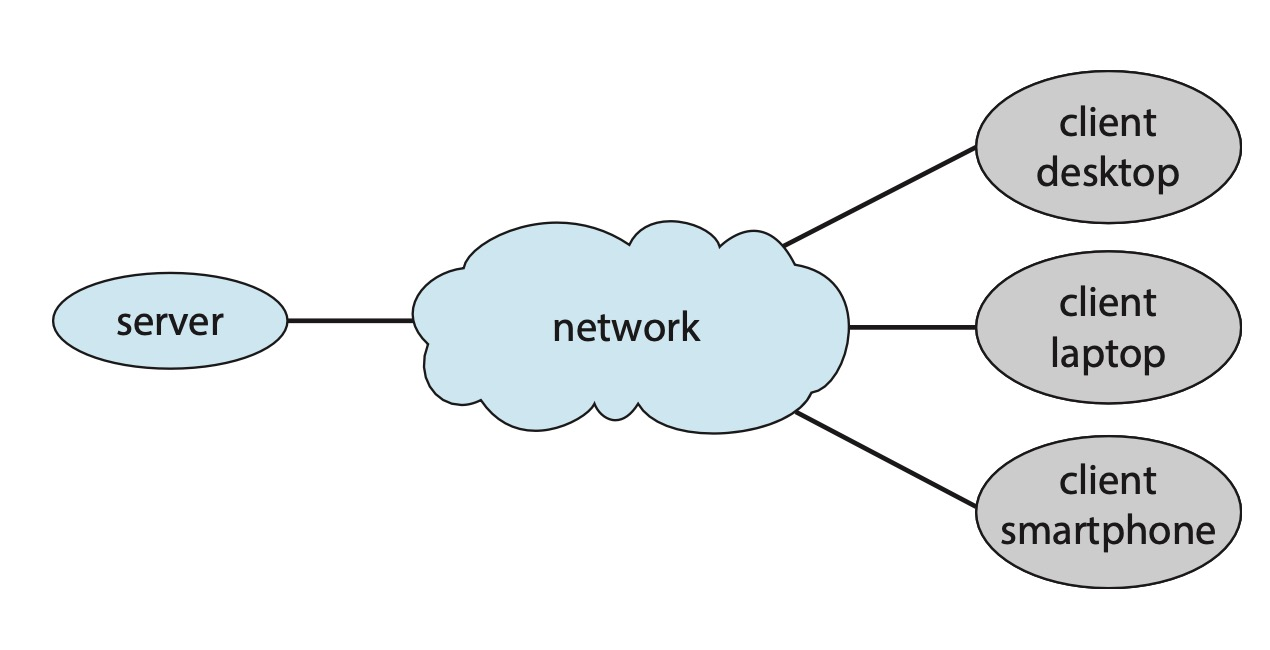
\includegraphics[width=1\linewidth]{assets/client-server.jpg}
        \end{figure}
    \end{minipage}
\end{figure}

\begin{figure}[H]
    \begin{minipage}{0.55\textwidth}
        \subsubsection*{Modello Peer to peer}
        Un modello distribuito peer to peer non fa distinzioni tra client e server, è invece costituita da nodi equivalenti che fungono sia da client che da server rispetto agli altri elementi della rete.

        \spacer

        Quando un nuovo dispositivo vuole entrare in un network peer to peer deve registrare il suo servizio in un registro centralizzato di consultazione della rete. Quando un nodo vuole connettersi con un'altro della rete deve prima contattare il registro centralizzato.
    \end{minipage}
    \hfill
    \begin{minipage}{0.35\textwidth}
        \begin{figure}[H]
            \centering
            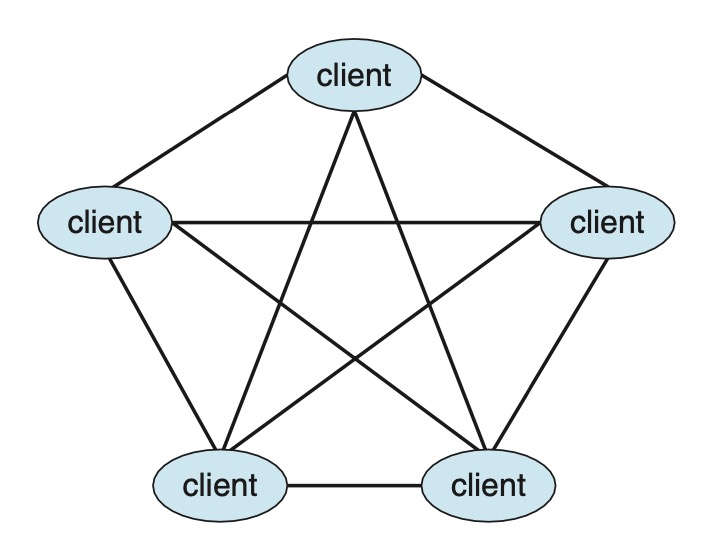
\includegraphics[width=0.9\linewidth]{assets/peer-to-peer.jpg}
        \end{figure}
    \end{minipage}
\end{figure}

\subsubsection*{Cloud Computing}
Il cloud computing è una teconologia che permette di accedere a risorse computazionali, di storage e di applicazione attraverso i servizi di rete.
Risulta particolarmente utile e comodo su dispositivi mobili, le cui risorse sono fortemente limitate.

\spacer
\begin{sitemize}
    \item \textbf{Cloud Pubblico:} liberamente disponibile tramite internet a chi si abbona al servizio
    \item \textbf{Cloud Privato:} gestito da un'azienda per utilizzo interno.
    \item \textbf{Cloud Ibrido:} contiene componenti pubbliche e private.
    \item \textbf{Infrastructure as a service (IaaS):} server o memoria disponibili attraverso l'internet.
    \item \textbf{Platform as a service (PaaS):} un ambiente software il cui hardware viene gestito e che permette di costruire applicativi facilmente.
    \item \textbf{Software as a Service (SaaS):} un'applicazione fruibile tramite internet (es. google docs).
\end{sitemize}

\begin{figure}[H]
    \centering
    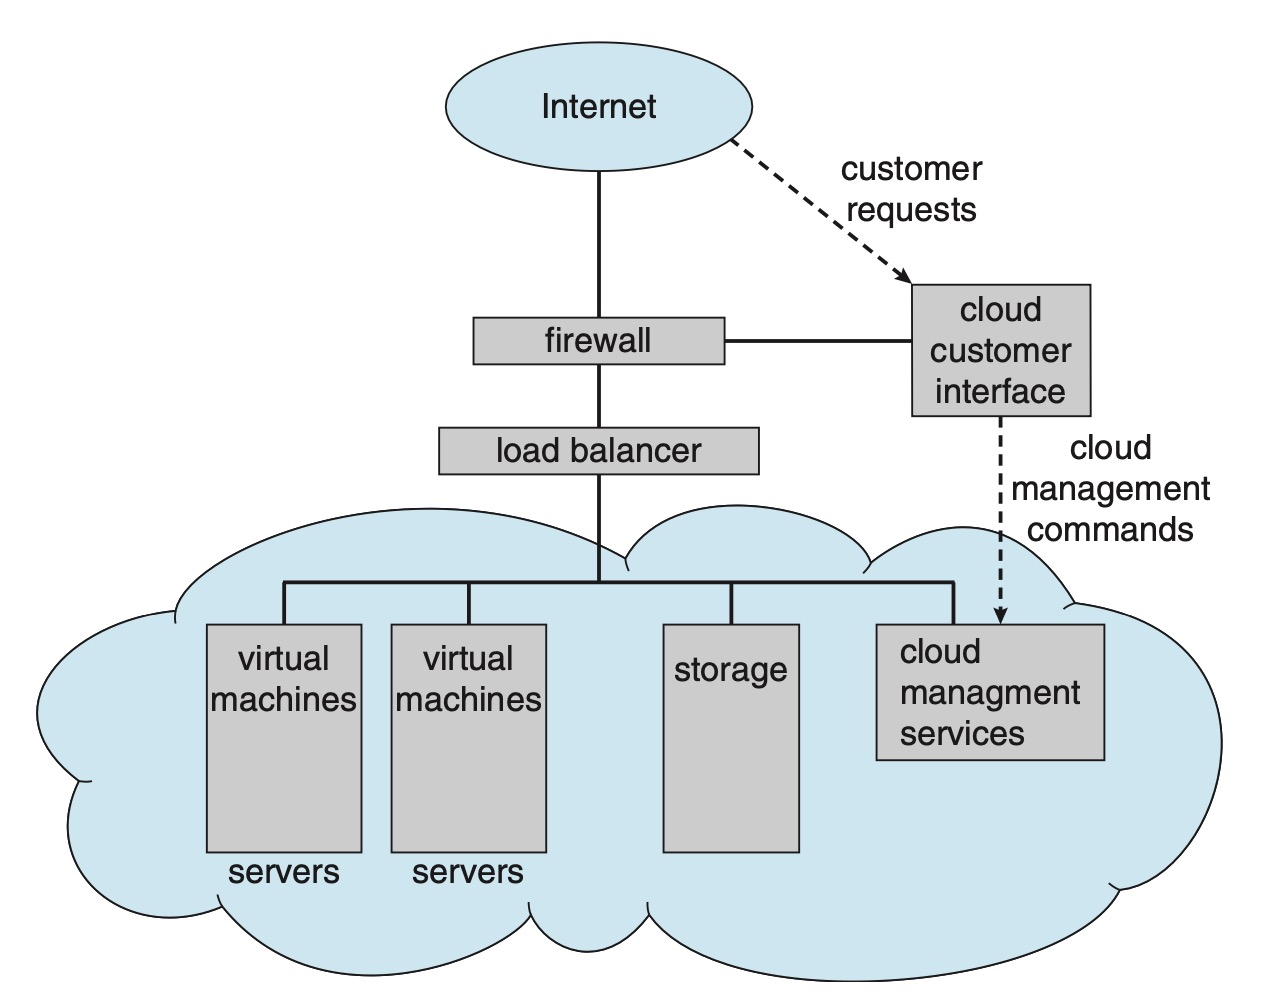
\includegraphics[width=0.35\linewidth]{assets/cloud-computing.jpg}
\end{figure}

\subsubsection*{Sistemi embedded}
Sono gli elaboratori largamente più diffusi, si possono trovare ovunque nelle nostre case.

Sono sistemi rudimentali, hanno compiti precisi, funzionalità limitate e un'interfaccia utente minimale, se presente.

\spacer
Possiamo trovare una grande variabilità tra i sistemi embedded:
\begin{sitemize}
    \item Alcuni sono \textbf{general-purpose} con un sistema operativo standard e delle applicazioni create appositamente per implementare una funzionalità.
    \item Microprocessori con un sistema operativo \textbf{special-purpose} che implementa solamente la funzionalità.
    \item Altri ancora hanno solamente dei \textbf{circuiti} costruiti appositamente per la funzionalità e sono privi di sistema operativo.
    \item \textbf{Sistemi Operativi Real-time}
\end{sitemize}

\spacer
Questi ultimi sono la tipologia più diffusa di sistemi embedded, si utilizza quando il tempo a disposizione per la lettura, l'elaborazione dei dati e l'esecuzione è fissato.

Nel caso in cui il sistema non riesca a produrre una risposta nel tempo prefissato essa verrà considerata errata.

\section{Sistemi Operativi Open Source}
Sono sistemi operativi disponibili in \textbf{formato sorgente} anziché come codice binario.

Questo approccio ha il vantaggio di aprire il sistema ad una vasta rete di programmatori, i quali sono liberi di contribuire al software aggiungendo funzionalità e risolvendo bug e falle di sicurezza.

\begin{note}
    È da notare che software opensource e free non sono sinonimi. Il software libero permette l'utilizzo, la redistribuzione e la modifica senza costo, mentre quello opensource può avere delle licenze che limitano la libertà degli sviluppatori.
\end{note}

\subsubsection*{Storia del Software Libero}
Il codice viene inizialmente concepito come libero, i primi sviluppatori dell'MIT lasciavano i loro codici sorgenti nei cassetti per lasciare che altri continuassero il lavoro.

\spacer
Durante gli anni 70 e 80 però le aziende iniziano a cercare modi per permettere l'esecuzione del loro software ai soli clienti paganti, quindi iniziano a distribuire i file compilati invece del codice sorgente.

\spacer
Per combattere questo spostamento verso il software proprietario, nel 1984 \textit{Richard Stallman} inizia a sviluppare un sistema operativo libero, compatibile e simile a Unix (il sistema operativo più diffuso al tempo), chiamato GNU (acronimo ricorsivo di \textit{\textbf{G}NU's \textbf{N}ot \textbf{U}nix!}).

\spacer
Stallman non è contrario all'idea di mettere un prezzo al proprio software, ma crede che i clienti debbano avere 4 libertà:
\begin{sitemize}
    \item \textbf{Eseguire} liberamente il programma
    \item Studiare e \textbf{modificare} il codice sorgente
    \item \textbf{Ridistribuire} o vendere il codice senza modifiche
    \item \textbf{Ridistribuire} o vendere il codice con delle modifiche
\end{sitemize}

\spacer
Nel 1985 Stallman pubblica il manifesto di GNU che suggerisce che tutto il software dovrebbe essere libero e fonda la \textit{Free Software Foundation (FSF)} con lo scopo di incoraggiare l'uso e lo sviluppo di software libero.

Stallman applica il "copyleft", ovvero l'esatto opposto del copyright, a tutto il suo lavoro che lo rende completamente libero, con l'unica condizione che debba essere ridistribuito come software libero.

Questo ideale viene poi sintetizzato nella \textit{GNU General Public License (GPL)}

\spacer
Nel 1991 il progetto GNU aveva sviluppato molti tool per lo sviluppo, ma non era ancora arrivato ad un kernel completo. Linus Torvalds, uno studente Finlandese, inizia a sviluppare un sistema operativo usando gli strumenti sviluppati dal progetto GNU.

Grazie anche all'avvento di internet, che permette a sviluppatori da tutto il mondo di scaricare il codice sorgente e di contribuire attivamente al progetto, nasce il sistema operativo \textit{Linux}.

\spacer
Dal kernel nascono moltissime distribuzioni, ogniuna con i suoi obiettivi e le sue particolarità.

\begin{note}
    \textbf{MINIX} è uno dei sistemi operativi più diffusi, anche se raramente ne sentiamo parlare. È stato sviluppato dal professor Andrew Tanenbaum come supporto didattico al suo corso universitario, con la caratteristica di essere estremamente modulare.

    Il sistema operativo è così diffuso perché intel lo utilizza per L'Intel Managment Unit, un software che viene eseguito da tutti i processori intel. Il sistema viene eseguito al livello di privilegio più elevato, con permessi pressoché illimitati sull'hardware.
\end{note}
\chapter{Strutture dei Sistemi Operativi}
Analizziamo ora le regole e gli strumenti necessari per l'implementazione di un sistema operativo.

Esso è un sistema complesso, è quindi fondamentale definire correttamente i requisiti. Essi si possono definire da vari punti di vista: i servizi che dovrà fornire, l'interfaccia messa a disposizione agli utenti e ai programmatori.

\section{Servizi}

Alcune classi di servizi che il sistema operativo può fornire nei confronti dell'utente:
\begin{sitemize}
    \item \textbf{Interfaccia Utente:}

    Quasi tutti i sistemi operativi sono dotati di un'interfaccia utente, che può prendere molte forme diverse, la linea di comando, un'interfaccia grafica, ...

    Si può interagire con essa in molti modi, con mouse e tastiera, con uno schermo touch, ...

    \item \textbf{Esecuzione di Programmi:}

    Il sistema deve essere in grado di caricare un programma in memoria ed eseguirlo, inoltre deve essere in grado di rilevare e gestire situazioni di errore.

    \item \textbf{Operazioni I/O:}

    Il sistema operativo fornisce ai programmi dell'utente un modo per accedere ai dispositivi I/O.

    \item \textbf{Gestione del File-System:}

    I programmi utente devono essere in grado di creare, leggere, scrivere ed eliminare file e devono potersi muovere nella struttura dell'archiviazione.

    \item \textbf{Comunicazioni:}

    I programmi devono essere in grado di comunicare ad altri processi presenti sullo stesso sistema oppure ad altri sistemi connessi via rete.
    La comunicazione può essere implementata tramite memoria condivisa, oppure come scambio di messaggi

    \item \textbf{Rilevamento di Errori:}

    Il sistema operativo deve tenere sotto costante controllo CPU, memoria e dispositivi I/O per rilevare e gestire gli errori che sorgono durante l'esecuzione dei programmi utente.
\end{sitemize}

\spacer
Ci sono altri servizi che il sistema operativo deve eseguire per assicurarsi che il sistema funzioni in modo efficiente:

\begin{sitemize}
    \item \textbf{Allocazione di Risorse:}

    Quando ci sono più processi o più utenti diventa fondamentale gestire in modo efficiente le risorse hardware tra di essi, in particolare la CPU e la memoria.
    I dispositivi I/O spesso vengono gestiti in modo meno rigido utilizzando delle regole generali.

    \item \textbf{Logging:}

    Risolta essere importante registrare quali programmi e in quali quantità utilizzano le risorse del sistema.
    Queste statistiche sono preziose per gli amministratori che possono capire l'effettiva necessità di risorse.

    \item \textbf{Protezione e Sicurezza:}

    Ai possessori di informazioni su un sistema multiutente o distribuito deve essere garantito i propri dati da accessi indesiderati.

    La protezione riguarda il controllo di tutti gli accessi alle risorse di sistema.

    La sicurezza si basa sull'obbligo di autenticazione mediante password o sistema equivalente.
\end{sitemize}

\subsection{Interfaccia Utente}
Vista la sua importanza dal punto di vista dell'utente può essere utile approfondire le interfacce che permettono agli utenti di comunicare con il sistema operativo.

\subsubsection*{Command Line Interpreter (CLI)}

L'interfaccia a linea di comando permette di impartire comandi direttamente al sistema operativo.
Viene talvolta implementata dal kernel oppure attraverso programmi di sistema, inoltre può essere anche installata dall'utente, il sistema operativo può offrire più \textit{shell}.

\spacer
I comandi impartiti dall'utente possono essere eseguiti secondo due modalità:

\begin{sitemize}
    \item Se il codice del comando è relativo all'interprete viene chiamata direttamente la funzione richiesta dall'utente.

    \item Se invece il codice del comando viene implementato da un altro programma di sistema l'interprete utilizza il comando per accedere al file contenente il codice per l'esecuzione e lo inizializza.
\end{sitemize}

\begin{note}
    Spesso nei sistemi operativi non sono disponibili tutte le funzionalità tramite l'interfaccia grafica, in questi casi si può accedervi tramite l'interprete a linea di comando.

    \spacer[4pt]
    Inoltre la linea di comando risulta essere utile per l'esecuzione di comandi ripetuti in quanto è programmabile
\end{note}

\subsubsection*{Graphical User Interface (GUI)}

L'interfaccia grafica user-friendly realizza la metafora della scrivania (\textit{desktop}).

L'utente può muovere un cursore su icone che rappresentano programmi, file, cartelle e funzioni di sistema.

Questo rende semplice l'interazione con il sistema tramite mouse, tastiera e monitor.

\begin{note}
    L'interfaccia grafica nasce dal lavoro del centro di ricerca \textit{Xerox Palo Alto Research Center (PARC)}, le cui idee vennero poi riprese da Steve Jobs nella creazione del software per il primo Machintosh.

    \spacer[4pt]
    Gli sviluppatori di apple non hanno però mai avuto accesso al codice, quindi provarono ad ricrearlo partendo da una semplice dimostrazione, nella maggior parte delle situazioni riusciranno addirittura a migliorare le funzionalità del sistema della Xerox.

    \spacer[4pt]
    La storia ha un triste epilogo con la Xerox che provò a fare causa ad apple sul copyright dell'interfaccia, ma una corte statunitense porrà fine alla causa un anno dopo scagionando apple.
\end{note}

\section{Chiamate di Sistema}
Le chiamate di sistema forniscono un'interfaccia tra i programmi e i servizi offerti dal sistema operativo.

Questo permette al programmatore di chiamare le funzioni da linguaggi di programmazione ad alto livello (C o C++) anche se l'implementazione può essere stata fatta ad esempio in assembly.

\subsection{Implementazione}
Dal punto di vista implementativo viene assegnato un numero ad ogni \textit{system call} e il sistema operativo tiene una tabella che associa numeri al codice che gestisce la chiamata a sistema.

\begin{figure}[H]
    \centering
    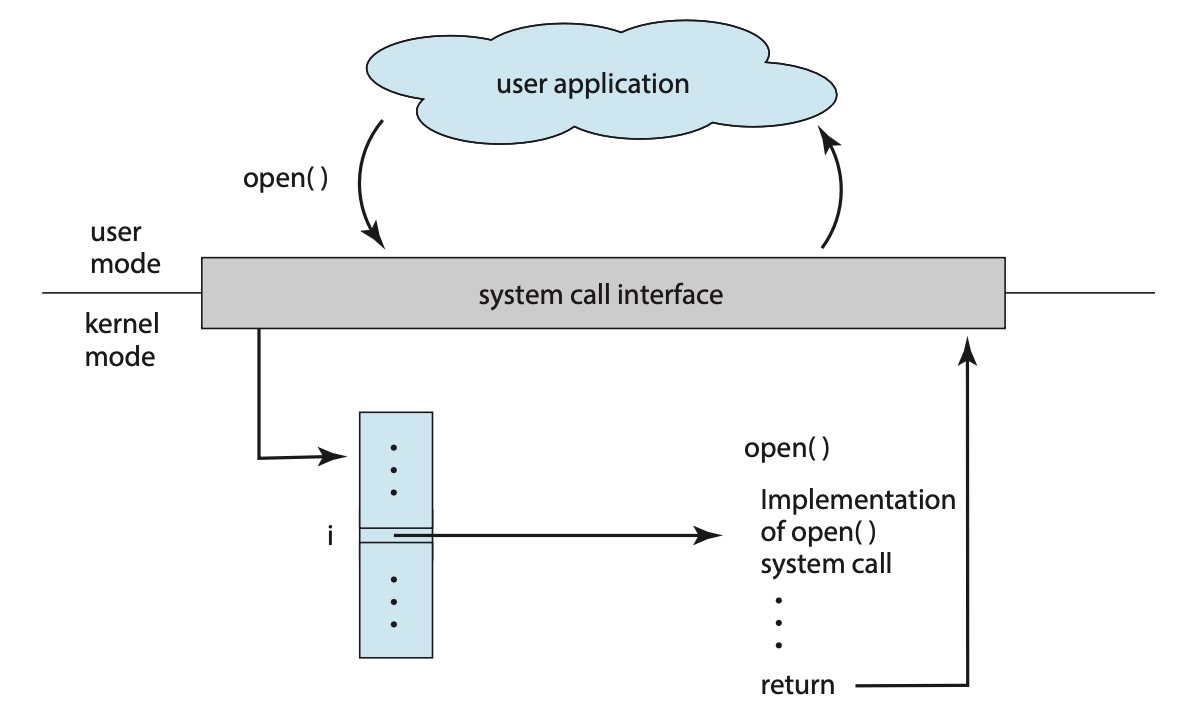
\includegraphics[width=0.65\linewidth]{assets/systemcall.jpg}
    \caption{La gestione della chiamata a sistema \texttt{open()}}
\end{figure}

Spesso è necessario fornire più informazioni della semplice chiamata. Il tipo e la quantità di dati che devono essere forniti alla \textit{system call} possono variare molto.

\spacer
Ci sono diverse soluzioni a questo problema:
\begin{sitemize}
    \item \textbf{Utilizzare i registri}, per quanto sia il metodo più semplice, limita numero e dimensione dei parametri.
    \item Memorizzazione dei parametri su un \textbf{blocco di memoria} e passaggio dell'indirizzo del blocco utilizzando un registro (Linux e Solaris).
    \item \texttt{Push} dei parametri nello \textbf{stack} da parte del programma e poi \textit{}t{pop} da parte del sistema operativo.
\end{sitemize}

\subsection{Application Programming Interface}
Gli sviluppatori spesso non vedono l'implementazione di queste funzioni, che spesso risultano essere estremamente complesse anche per azioni relativamente semplici.

I programmi e i loro sviluppatori interagiscono con delle \textit{Application Programming Interface (API)}, un set di funzioni che sono disponibili al programmatore.

\spacer
L'utilizzo di un'API permette all'utente di non preoccuparsi dei dettagli implementativi e permette una maggiore portabilità del programma ad altri sistemi operativi.

\begin{note}
    Alcune delle API più diffuse ed utilizzate sono la \textit{Win64 API} per Windows, \textit{POSIX API} per Unix, Linux e MacOS e la \textit{Java API} per la \textit{Java Virtual Machine}.
\end{note}

\subsection{Tipologie di Chiamate a Sistema}

Le chiamate a sistema possono essere approssimativamente raggruppate in 6 categorie principali:
\begin{sitemize}
    \item \textbf{Controllo dei Processi:}

    Permette di creare, caricare, eseguire, far attendere e terminare un processo. Inoltre permette di leggere e modificare gli attributi del processo (priorità, tempo di esecuzione, $\ldots$), assegnare/rilasciare memoria e inviare segnali.

    \item \textbf{Gestione delle informazioni:}

    Permette di ottenere informazioni di sistema, la lettura/modifica dell'ora e della data, la lettura/modifica degli attributi di processi, file e dispositivi.

    \item \textbf{Comunicazione:}

    Permette l'apertura/chiusura di una connessione, l'invio/ricezione di messaggi, inserimento/esclusione di dispositivi remoti, condivide informazioni sullo stato dei trasferimenti e gestisce la condivisione della memoria.

    \item \textbf{Gestione dei file:}

    Permette la creazione/eliminazione/apertura/chiusura/lettura/scrittura di file e condivide gli attributi dei file.

    \item \textbf{Gestione dei dispositivi I/O:}

    Permette la richiesta e rilascio di un dispositivo, la lettura e scrittura dei dati e condivide gli attributi di un dispositivo.
\end{sitemize}

\section{Programmi di Sistema}
I programmi di sistema forniscono un ambiente conveniente per lo sviluppo e l'esecuzione di programmi.

In alcuni casi possono essere semplici interfacce per chiamate a sistema, altre volte possono essere più complesse.

\spacer
Alcuni possibili scopi dei programmi di sistema sono:

\begin{sitemize}
    \item \textbf{Gestione di file}
    \item \textbf{Modifica di file}
    \item \textbf{Informazioni di stato}
    \item \textbf{Supporto a linguaggi di programmazione} (compilatori, debugger, $\ldots$)
    \item \textbf{Caricamento ed esecuzione dei programmi}
    \item \textbf{Comunicazioni}
    \item \textbf{Servizi background}

    Sono programmi che vengono lanciati al boot, alcuni terminano dopo aver completato alcune azioni, altri continuano ad essere eseguiti fino allo spegnimento.

    Supportano servizi quali il controllo del disco, scheduling dei processi, logging degli errori, stampa, connessioni di rete, $\ldots$

    \item \textbf{Programmi applicativi}

    Sono Programmi che non fanno parte del sistema operativo (es. browser, editor di testo, $\ldots$), ma sono importanti per l'esperienza degli utenti.
\end{sitemize}

\subsection{Linkers e Loaders}

Dal file sorgente un \textbf{compilatore} crea un file oggetto, il quale è progettato per essere caricato in qualsiasi locazione di memoria.

Poi il \textbf{linker} crea il file eseguibile, combinando i file oggetto e le librerie necessarie.

Il file così generato è pronto per essere caricato in memoria da un \textbf{loader}.

\spacer

I file oggetto ed eseguibili devono avere un formato standard per poter comunicare al sistema operativo come caricare ed eseguire il programma.

Per i sistemi UNIX-like il formato standard è l'\textit{Executable and Linkable Format (ELF)}, per Windows è il formato \textit{PE}, per macOS \textit{Mach-O}.
\begin{figure}[H]
    \centering
    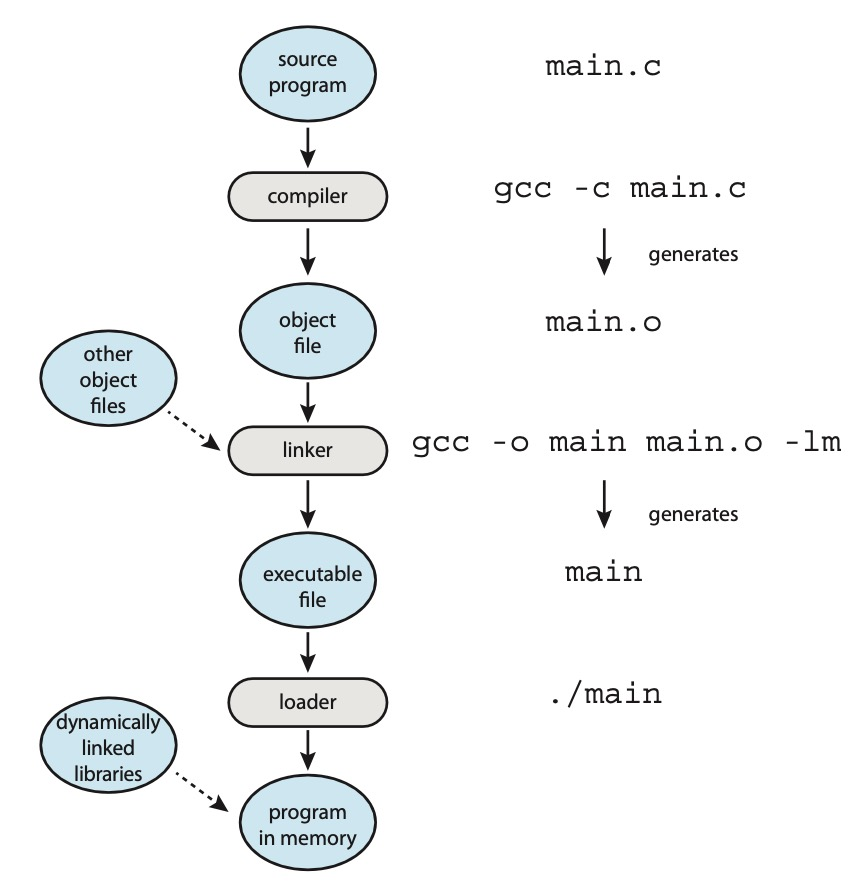
\includegraphics[width=0.38\linewidth]{assets/linker-loader.jpg}
\end{figure}

\begin{note}
    I moderni sistemi operativi \textit{general purpose} non compilano le librerie nei file eseguibili, utilizzano piuttosto delle librerie collegate dinamicamente (es. DLL per Windows) secondo le necessità e condivise da tutti i programmi.
\end{note}

\subsubsection{Le applicazioni sono OS-specific}
Le applicazioni compilate per un sistema \textbf{non} possono, in generale, essere eseguite su altri sistemi. Se questo fosse possibile non dovremmo scegliere il sistema operativo in base agli applicativi che sono disponibili, ma in base alle funzionalità del sistema.

\spacer
Parte del problema, che rende difficile l'interoperabilità tra sistemi, è che ognuno ha il suo \textbf{set di chiamate} a sistema, i propri formati di file eseguibili, ...

\spacer
Ci sono alcune soluzioni per scrivere codice che può essere eseguito su più sistemi:
\begin{itemize}
    \item Scrivere in un \textbf{linguaggio interpretato}, come Python, in questo caso è sufficiente che esista un interprete disponibile per quel sistema operativo.

    \item Scrivere in un linguaggio che \textbf{include una VM} all'interno della quale avviene l'esecuzione, come Java.

    \item Scrivere in un \textbf{linguaggio standard}, come C, e compilare poi per ogni sistema.
\end{itemize}

\subsubsection{ABI}
Proprio come le API permettono al programmatore di non dover programmare le implementazioni di semplici funzioni in codice macchina, le ABI forniscono al compilatore il set di istruzioni che possono essere eseguite sulla specifica architettura per cui si sta compilando.

\spacer
Il problema è che le ABI spesso non forniscono una gran quantità di interoperabilità, quindi il codice deve essere compilato \textbf{per ogni sistema operativo} e \textbf{per ogni architettura} su cui verrà eseguito.

\section{Implementazione di un Sistema Operativo}

Tradizionalmente i sistemi operativi venivano scritti in assembly, successivamente vennero utilizzati dei linguaggi specifici e ad oggi si utilizza principalmente C o C++ per scrivere il \textit{kernel}, assieme a frammenti in assembly per gli elementi di basso livello.

\spacer
Vista la complessità del codice richiesto da un sistema operativo è importante pensare alla struttura da impartire ad esso, vediamo ora le strutture più comune che vengono usate per la creazione dei sistemi operativi.

\begin{figure}[H]
    \centering
    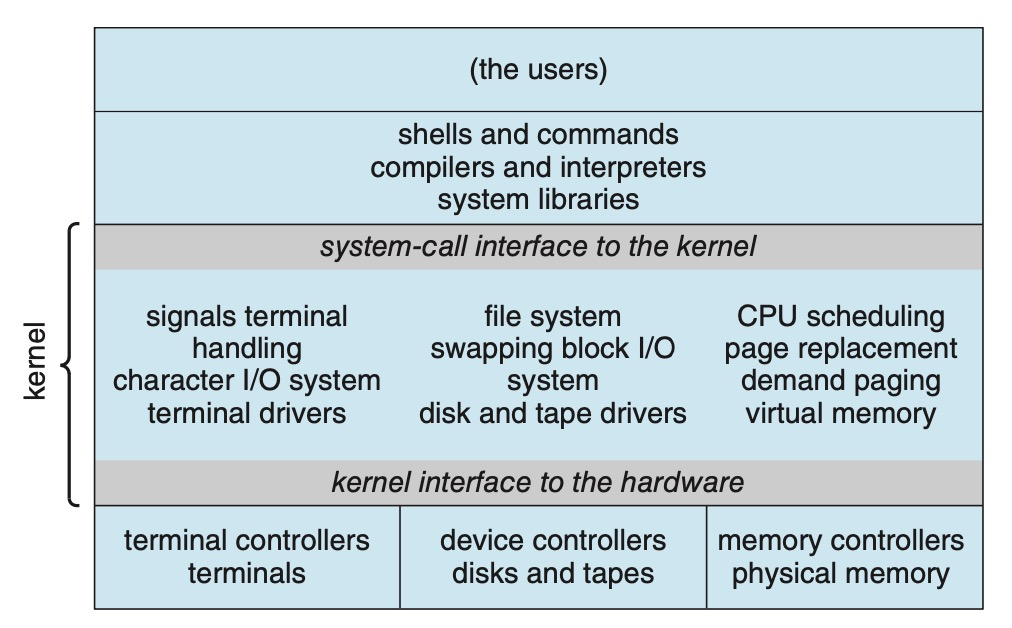
\includegraphics[width=0.55\linewidth]{assets/os-structure.jpg}
\end{figure}

\subsection{Design di un Sistema Operativo}
Abbiamo già visto come vengono definiti gli obiettivi del sistema operativo, vedendo cosa gli utenti e l'hardware si aspettano da esso.

\spacer

Nella progettazione di un software complesso come il sistema operativo è importante mantenere separati i due concetti di politiche e meccanismi.

Le \textbf{politiche} definiscono i compiti e servizi che il sistema operativo deve fornire, mentre i \textbf{meccanismi} definiscono come queste politiche andranno implementate all'atto pratico.

\begin{note}
    In macos e Windows politiche e meccanismi sono fissati a priori e scritti nel sistema, in Linux la separazione tra le due è più evidente.
\end{note}

\subsection{Monolitici}
La struttura più semplice è l'\textbf{assenza di una struttura}. Tutta la funzionalità del kernel viene implementata in un unico eseguibile, con tutte le funzioni strettamente collegate.

\spacer
Questo significa che un singolo bug in uno dei sistemi può comportare il blocco dell'intero sistema, inoltre lo sviluppo e l'estensione risultano essere particolarmente complicati per un kernel monolitico.

Tuttavia quando costruito in modo sicuro la stretta integrazione rende il sistema \textbf{estremamente efficiente}.

\begin{note}
    MS-DOS non implementava una struttura modulare, le applicazioni fanno chiamate a system call direttamente, aprendo così la strada a diverse vulnerabilità.

    \spacer
    Anche UNIX implementava un kernel parzialmente monolitico, con l'obiettivo di migliorare le performance.
    Esso presentava solo due livelli, il kernel e le applicazioni utente. Lo strato del kernel si ritrova con una gran quantità di responsabilità.

    \begin{figure}[H]
        \centering
        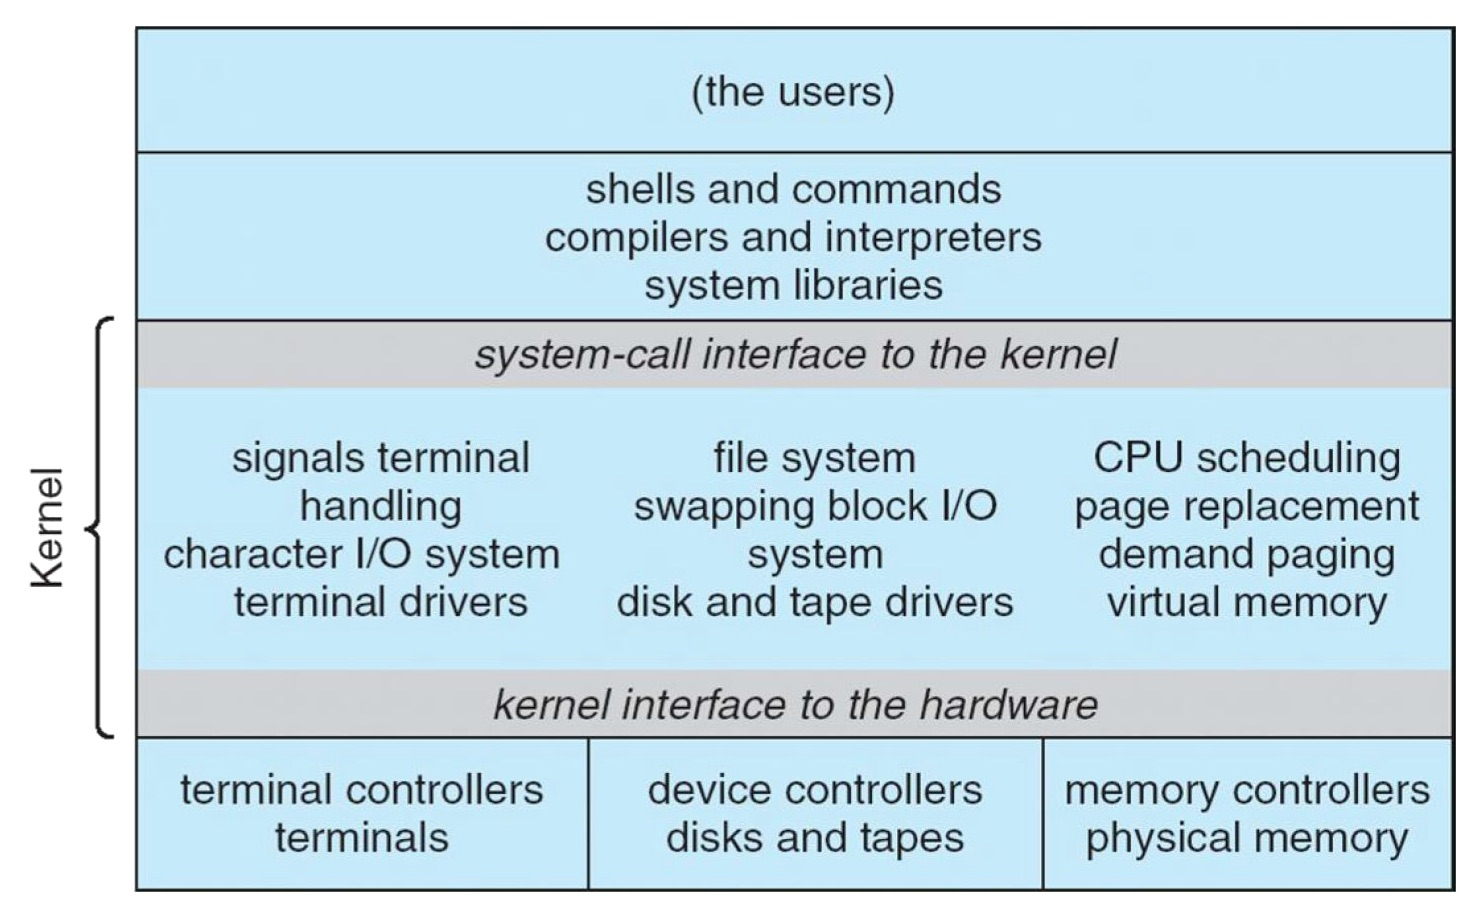
\includegraphics[width=0.5\linewidth]{assets/unix-monolithic.jpeg}
    \end{figure}
\end{note}

\subsection{Approccio stratificato}
L'alternativa all'approccio monolitico è un approccio dove i vari sistemi sono separati in componenti o moduli relativamente piccoli che assieme compongono il kernel.

\spacer
Uno dei modi per implementare un approccio modulare è quello stratificato, in presenza di hardware appropriato è possibile suddividere le funzioni del sistema operativo su vari \textbf{livelli}. Il livello 0 è l'hardware, il livello N è l'interfaccia utente.

Ciascuno strato impiega esclusivamente funzioni degli strati di livello inferiore.

\spacer
Questa struttura ha il vantaggio di facilitare la realizzazione e messa a punto del sistema operativo.

Gli svantaggi invece sono legati ai tempi di attraversamento dei vari strati (si pensi ad una system call che deve essere intercettata e riportata da molteplici livelli) e alla difficoltà di definire gli strati, in quanto essi possono usare solo le funzioni degli strati inferiori (si pensi al driver della memoria virtuale, che dovrebbe essere sopra allo scheduler, perché deve essere possibile interromperne l'esecuzione in caso di page fault. Ma allo stesso tempo lo scheduler deve essere a conoscenza delle informazioni del driver per poter gestire al meglio i processi).

\begin{figure}[H]
    \centering
    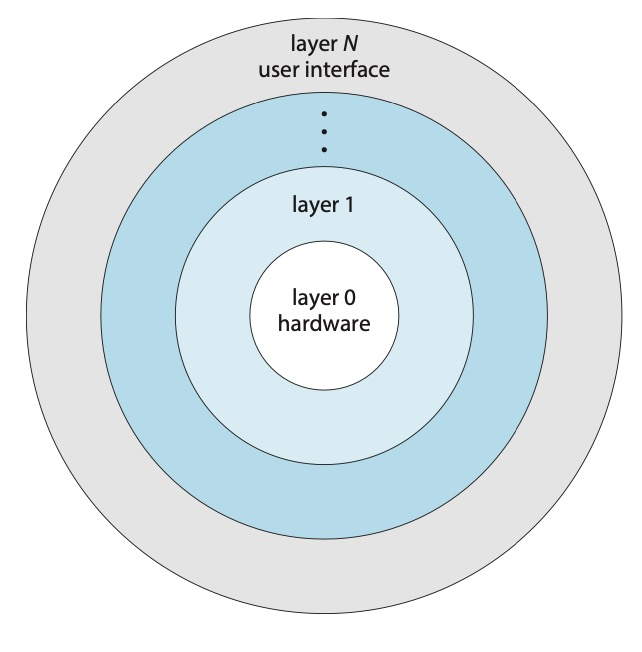
\includegraphics[width=0.4\linewidth]{assets/os-layered.jpg}
\end{figure}

\subsection{Microkernel}
Un microkernel offre la \textbf{minima quantità di servizi} di gestione dei processi, della memoria e di comunicazione.

Tutte le funzionalità non essenziali al kernel sono implementate come programmi utente, c'è quindi necessità di intensa comunicazione tra le varie componenti, cosa che viene mediata dal kernel.

\spacer
Il microkernel è semplice da modificare e rende semplice aggiungere e modificare le funzionalità, in quanto esse sono implementate a livello utente.

Inoltre i sistemi operativi con microkernel sono più sicuri (meno codice viene eseguito a livello kernel) e sono più facili da portare a nuove architetture.

Il più grande svantaggio è l'\textbf{overhead} di prestazioni causato dalle continue comunicazioni tra i moduli.

\begin{figure}[H]
    \centering
    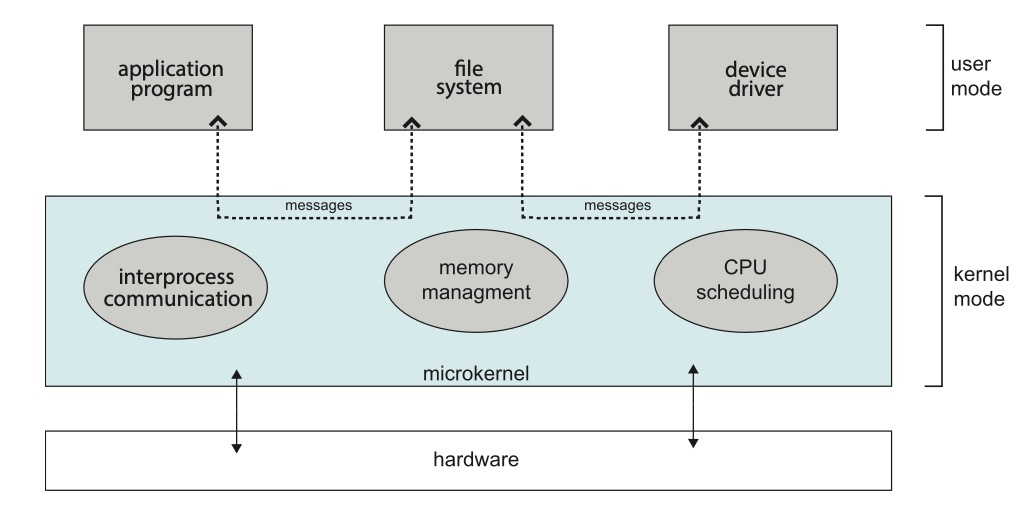
\includegraphics[width=0.5\linewidth]{assets/microkernel.jpg}
\end{figure}

\begin{note}
    Utilizzato da alcuni sistemi operativi più vecchi, come le prime versioni di Windows NT o macOS su kernel darwin.
\end{note}

\subsection{Kernel Modulari}
L'implementazione di tutti i moderni sistemi operativi utilizza i \textit{Loadable Kernel Module (LKMs)}.
Si utilizza un approccio object-oriented dove ciascun modulo implementa un'interfaccia che definisce una funzione del kernel.

Ciascun modulo può comunicare con gli altri moduli mediante l'interfaccia comune, inoltre ogni modulo può essere caricato o meno in memoria in base alle necessità.

\spacer
Questo approccio è simile a quello del microkernel con solo alcuni moduli caricati inizialmente che hanno il compito di caricare gli altri in base alla necessità, ma vengono risolti i problemi di comunicazione.

\subsection{Sistemi ibridi}
Nei sistemi operativi moderni si utilizza spesso un approccio misto rispetto a quelli visti precedentemente.

\subsubsection*{Linux}
Linux ha un kernel principalmente monolitico per poter fornire prestazioni elevate, tuttavia esso può essere anche esteso in modo dinamico.

\subsubsection*{Windows}
Anche Windows è in larga parte monolitico, ma conserva alcune caratteristiche tipiche dei sistemi microkernel tramite il supporto per sottosistemi (\textit{personalities}) che vengono eseguiti a livello utente.

\subsubsection*{macOS e iOS}
Anche se i sistemi possono sembrare molto differenti e vengono eseguiti su architetture e dispositivi diversi, essi condividono una struttura simile.

\spacer
\begin{sitemize}
    \item \textbf{User experience (GUI):} Permette l'interazione col software, diversa per macOS e iOS in base allo stile di input.
    \item \textbf{Ambienti applicativi:} Cocoa fornisce le API per i linguaggi di programmazione Objective-C e Swift.
    \item \textbf{Framework di base:} Ambienti che supportano le API grafiche e di base, come OpenGL.
    \item \textbf{Ambiente kernel:} Darwin include il kernel BSD UNIX, è estendibile grazie ai kext utili allo sviluppo di driver ed estensioni del kernel.
\end{sitemize}
\spacer

Le applicazioni su questi sistemi possono essere progettate per sfruttare le funzionalità di user experience o per aggirarle completamente (disponibile ai developer solo su macOS).

\begin{figure}[H]
    \centering
    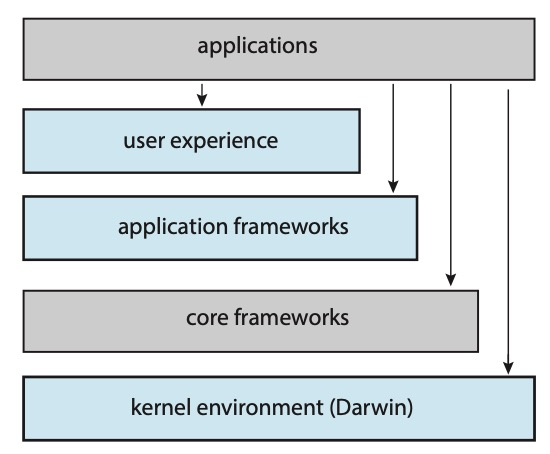
\includegraphics[width=0.4\linewidth]{assets/apple-os-structure.jpg}
    \caption{Struttura dei sistemi macOS e iOS}
\end{figure}

\subsubsection*{Android}
Sviluppato dalla \textit{Open Headset Alliance} di cui Google fa parte, ma non è l'unica grande azienda, Android è un sistema operativo open source che gestisce una gran quantità di dispositivi mobili.

\spacer

Android nasce da una versione modificata del kernel linux, le applicazioni android sono scritte in Java e vengono poi eseguite sull'\textit{Android RunTime (ART)}.
Per migliorare le prestazioni ART non esegue una compilazione a tempo di esecuzione, ma viene eseguita all'installazione dell'applicazione.

Gli sviluppatori possono anche scegliere di utilizzare JNI, l'interfaccia nativa con un accesso più diretto all'hardware.

\begin{figure}[H]
    \centering
    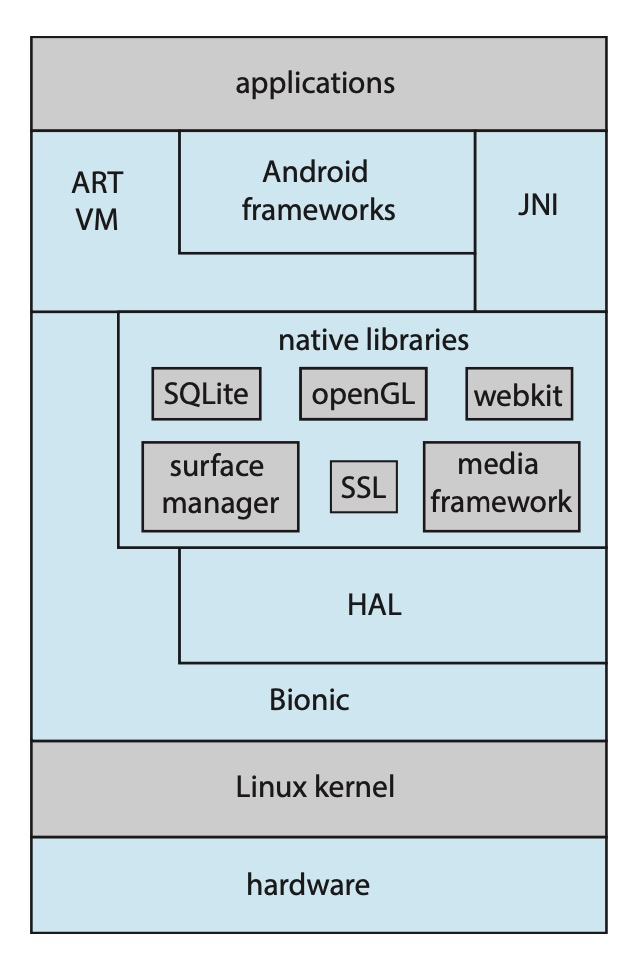
\includegraphics[width=0.27\linewidth]{assets/android.jpg}
    \caption{Struttura sistema android}
\end{figure}

\begin{note}
    Poiché i dispositivi android hanno specifiche hardware pressoché illimitato c'è un livello di astrazione tra l'hardware e le librerie native (\textit{Hardware Abstraction Layer, HAL})
\end{note}

\section{Debugging e Tuning}
Il \textbf{debugging} è l'attività di individuazione e risoluzione dei problemi, il che comprende sia la risoluzione dei bug che il performance tuning.

\spacer
Il sistema operativo aiuta nel processo con la generazione di \textbf{file di log} che danno informazioni sugli errori rilevati durante l'esecuzione.
Inoltre il sistema operativo fornisce un \textbf{core dump}, ovvero una copia della memoria impiegata dal processo al momento della terminazione anomala.

\begin{note}
    \textbf{Kernel}

    Quando avviene un errore al kernel viene chiamato \textbf{crash}. Quando questo avviene viene creato un \textbf{crash dump} che viene inserito in un'apposita sezione della memoria.

    \spacer
    È necessario di scrivere su un'area riservata di memoria perché quando si ottiene un crash lo stato del sistema non è garantito ed è difficile comprendere quali sezioni della memoria sono libere.
\end{note}

\subsection{Tuning}
Anche i problemi che condizionano le prestazioni sono considerati bachi e vanno quindi trovati e risolti.
Il performance tuning è l'insieme delle tecniche atte ad ottimizzare le prestazioni del sistema ed ad eliminare i colli di bottiglia.

\spacer
Per fare ciò ci sono varie tecniche, è possibile eseguire del codice che misuri le prestazioni del sistema e poi ne salvi i risultati su un file di log.

Oppure possono essere utilizzati degli strumenti grafici del sistema operativo, ad es. task manager di Windows.

Infine esiste anche il profiling che punta a visualizzare quali chiamate a sistema vengono utilizzare maggiormente così da ottimizzarle, quando possibile.
\chapter{Affidabilità}

Il capitolo viene svolto alla fine del corso nelle ultime slide, viene posizionato qui in quanto non rientra in nessuno dei macroargomenti del corso, ma riguarda il sistema in generale.

\section{Guasti}
I guasti possono avere una di due caratteristiche rispetto al tempo:
\begin{sitemize}
    \item \textbf{Temporanei:} Quindi guasti non sempre presenti in tutte le condizioni. Questi guasti possono essere transitori (avvengono una sola volta) oppure intermittenti (avvengono ad intervalli irregolari).

    \item \textbf{Permanenti:} Guasti che, una volta verificati, rimangono presenti finché il componente non viene sostituito o riparato.
\end{sitemize}

Invece rispetto alla loro importanza definiamo:
\begin{sitemize}
    \item \textbf{Guasti significativi:} guasti che degradano significativamente le prestazioni di un sistema.
    \item \textbf{Guasti maggiori:} Impediscono il completamento della missione.
\end{sitemize}

\subsubsection*{Tolleranza ai Guasti}
Una caratteristica importante di un sistema è la sua tolleranza ai possibili guasti che possono emergere, tipicamente richiede una qualche forma di ridondanza, con lo scopo di aumentare l'affidabilità del sistema.

\subsubsection*{Ridondanza}
\begin{sitemize}
    \item \textbf{Spaziale:} Richiede l'utilizzo di diversi componenti in grado di svolgere la stessa operazione, in modo da averne uno disponibile in caso di guasto.
    \item \textbf{Temporale:} Ritentare l'operazione quando si incontra un errore, permette di risolvere i guasti temporanei.
    \item \textbf{Informazione:} I dati vengono scritti in modo che possano verificare e correggere i possibili errori.
\end{sitemize}

\section{Affidabilità}
Si definisce affidabilità di un dispositivo la probabilità che esso funzioni correttamente, per un dato tempo, date certe condizioni.

\spacer
\begin{sitemize}
    \item \textbf{Affidabilità logistica:} Si riferisce alla probabilità che nessun guasto si verifichi
    \item \textbf{Affidabilità di missione:} Probabilità che non si verifichino guasti "gravi", ovvero tali da pregiudicare le funzionalità del sistema.
    \item \textbf{Sicurezza:} Probabilità che non si verifichino guasti con conseguenze catastrofiche, tali da produrre danni a persone e cose.
\end{sitemize}

\subsubsection*{Esempio}
\begin{center}
    \begin{tabular}{ | c | c | c | }
        \hline
        dispositivo & Ore di funzionamento & Minuti di riparazione \\
        \hline \hline
        1           & 490                  & 140                   \\
        2           & 760                  & 130                   \\
        3           & 2350                 & 80                    \\
        4           & 1400                 & 90                    \\
        5           & 1560                 & 110                   \\
        6           & 970                  & 150                   \\
        7           & 2300                 & 70                    \\
        8           & 1190                 & 90                    \\
        9           & 1130                 & 110                   \\
        10          & 300                  & 120                   \\
        \hline
        Somma:      & 12450                & 1090                  \\
        \hline
    \end{tabular}
\end{center}

\subsubsection*{Affidabilità:}

$$R(t) = \frac{n_{prod}(t)}{n_{prod}(t_o)}$$

dove $n_{prod}(t)$ è il numero di dispositivi funzionanti al tempo $t$.

\spacer
In questo caso $R(1000) = \frac{6}{10} = 0.6$

\subsubsection*{MTTF (Mean Time to Failure)}
$$MTTF = \frac{\sum_{n=1}^{N}T_n}{N}$$
dove $N$ è il numero di dispositivi

\spacer
In questo caso $MTTF = \frac{12450}{10} = 1245$ ore

\subsubsection*{MTTR (Mean Time to Repair)}
$$MTTR = \frac{\sum_{n=1}^{N}R_n}{N}$$
dove $N$ è il numero di dispositivi

\spacer
In questo caso $MTTR = \frac{1090}{10} = 109$ minuti

\subsubsection*{Availability}
Frazione di tempo in cui il dispositivo funziona correttamente.

$$A = \frac{MTTF}{MTTF + MTTR}$$

\spacer
In questo caso $A \approx 99.86\%$

\begin{note}
    Sia la funzione di affidabilità $R(t)$ che quella di guasto $Q(t) = 1-R(t)$ sono delle distribuzioni di probabilità.
\end{note}


\part{Gestione dei Processi}
\chapter{Threads e Concorrenza}
Abbiamo già visto nell'introduzione una prima definizione di processo, l'entità attiva di un programma. Vediamo ora più nel dettaglio l'evoluzione di esso nel tempo.

\section{Thread}
Un thread è l'unità fondamentale della computazione, può essere generato da un processo aprendo la possibilità alla \textbf{parallelizzazione} della task.

\spacer
I thread appartenenti allo stesso processo condividono codice, dati e risorse (ad es. una modifica ad una variabile globale oppure l'apertura di un file sono visibili a tutti i thread)

Queste situazioni vanno però gestite correttamente, altrimenti si rischia di di avere conflitti nell'accesso alle risorse.

\begin{figure}[H]
    \centering
    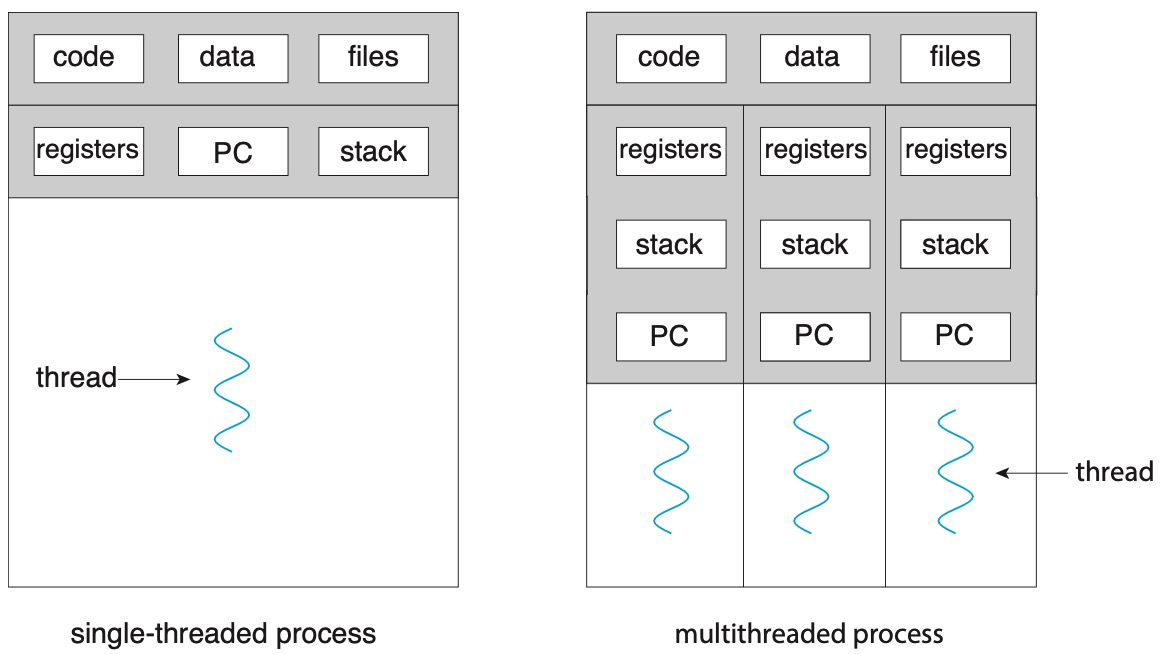
\includegraphics[width=0.6\linewidth]{assets/multithread.jpg}
\end{figure}

\spacer

Il thread comprende:
\begin{sitemize}
    \item un identificatore di thread
    \item un contatore di programma
    \item un insieme di registri
    \item uno stack
\end{sitemize}

\begin{note}
    Il processo tradizionale, che viene eseguito su un singolo processo, si definisce "\textit{heavyweight process}", mentre i thread sono detti anche "processi leggeri".

    \spacer[4pt]

    Un thread può essere utilizzato dal browser per rappresentare una singola pagina web, per generare velocemente icone per una serie di immagini oppure possono essere usati da un webserver, un thread per ogni richiesta.
\end{note}

\subsection{Visualizzazione}

Per visualizzare lo stato di un processo in relazione al tempo useremo dei grafici con il tempo sull'asse x, e lo stato del processo sull'asse y.

\begin{figure}[H]
    \centering
    \begin{minipage}{0.45\textwidth}
        \begin{tikzpicture}[scale=2.5]
            % assi
            \draw[->] (-0.1,0) -- (1.2,0) node[right] {$t$};
            \draw[->] (0,-0.1) -- (0,1.2) node[above] {$S$};

            % funzioni
            \draw[domain=0:0.5,smooth,variable=\x, line width=1.5pt] plot ({\x},{1.4*\x+1/10*sin(deg(12*\x))});
            \draw[domain=0.5:0.7,smooth,variable=\x, line width=1.5pt] plot ({\x},{0.672});
            \draw[domain=0.7:1,smooth,variable=\x, line width=1.5pt] plot ({\x},{ -2.65 + 7.3*\x - 3.65*\x^2});

            % riferimenti
            \draw[dashed] (0.5,0.672) -- (0.5, 0)  node[below] {$T_1$};
            \draw[dashed] (0.7, 0.672) -- (0.7, 0) node[below] {$T_2$};
            \draw[dashed] (1, 1) -- (1, 0) node[below] {$T_f$};
            \draw[dashed] (0.5, 0.672) -- (0, 0.672) node[left] {$S_1$};
            \draw[dashed] (1, 1) -- (0, 1) node[left] {$S_f$};
        \end{tikzpicture}

        In questo caso particolare si può notare un periodo di tempo, da $T_1$ a $T_2$ dove il processo rimane nello stato $S_1$, questo indica che si trovava in un \textit{bottleneck}, ovvero il processo stava attendendo una qualche risorsa.
    \end{minipage}
    \hfill
    \begin{minipage}{0.45\textwidth}
        \begin{tikzpicture}[scale=2.5]
            % assi
            \draw[->] (-0.1,0) -- (2.2,0) node[right] {$t$};
            \draw[->] (0,-0.1) -- (0,1.2) node[above] {$S$};

            % funzioni
            \draw[domain=0:1.018,smooth,variable=\x, line width=1.5pt] plot ({\x},{\x+1/10*sin(deg(6*\x))});
            \draw[domain=0:2.036,smooth,variable=\x, line width=1.5pt] plot ({\x},{0.5*\x+1/10*sin(deg(3*\x))});

            % riferimenti
            \draw[dashed] (1.018, 1) -- (1.018, 0) node[below] {$T_{f1}$};
            \draw[dashed] (2.036, 1) -- (2.036, 0) node[below] {$T_{f2}$};
            \draw[dashed] (2, 1) -- (0, 1) node[left] {$S_f$};
        \end{tikzpicture}

        In questo casolo stesso processo viene eseguito su due processori diversi, $T_{f1}$ è il processore più veloce, mentre $T_{f2}$ quello più lento.
    \end{minipage}
\end{figure}

\subsection{User e Kernel Threads}
Nei moderni sistemi operativi esistono threads al livello utente e altri al livello kernel.
Quando un thread a livello utente fa una chiamata a sistema è necessario trovare un thread a livello kernel che sia pronto ad accettarla, altrimenti si rischia di introdurre dei tempi di attesa.
Va quindi trovata una relazione tra le due tipologie di threads.

\subsubsection{One-to-One}
Mappa ogni thread a livello utente con un suo corrispettivo a livello kernel, questo assicura che ogni \textit{systemcall} venga gestita correttamente e rapidamente.
Tuttavia così facendo si creano molti thread che potrebbero portare ad una riduzione delle prestazioni.

\begin{figure}[H]
    \centering
    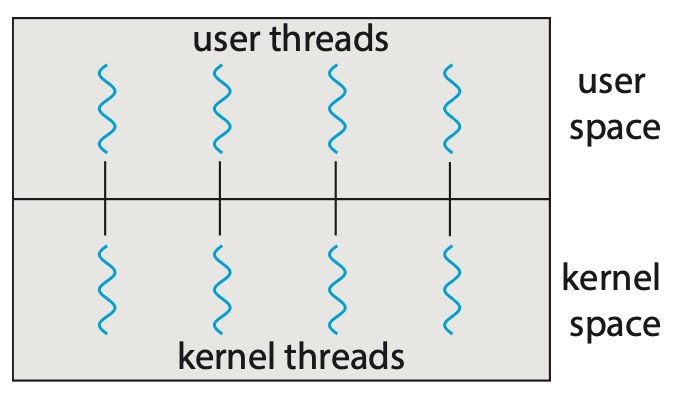
\includegraphics[width=0.35\linewidth]{assets/one-to-one.jpg}
\end{figure}

\subsubsection{Many-to-Many}
Questo modello mappa $n$ thread utente a $k$ thread kernel, dove $n << k$. Questo modello ha una migliore utilizzazione delle risorse, ma è di difficile realizzazione la funzione che associa thread utente a thread kernel.
Ad oggi nessun sistema operativo moderno lo utilizza, si preferisce usare il modello one-to-one.

\begin{figure}[H]
    \centering
    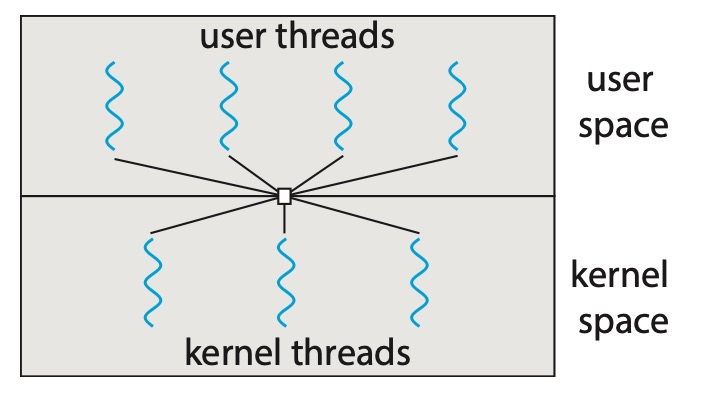
\includegraphics[width=0.35\linewidth]{assets/many-to-many.jpg}
\end{figure}

\subsection{Implementazioni}
\subsubsection{Linux}
Linux implementa la Process Control Block mediante una \textit{task struct}, la ready queue diventa quindi una lista concatenata di \textit{task struct}.

\spacer
Quando un processo crea uno o più figli può scegliere se continuare la sua esecuzione in parallelo con essi o se attendere la loro conclusione.

Inoltre può scegliere se eseguire lo stesso codice del genitore o un altro programma.

\spacer
In linux, come in molti altri Sistemi Operativi, tutti i processi sono figli di un processo iniziale, nel caso di linux è il processo con ProcessID = 1.

Un nuovo processo viene generato con la funzione texttt{fork()} che restituisce l'id del nuovo processo al parent e restituisce 0 al figlio, questo è importante perché permettere di distinguere se ci si trova nel parent o nel children.

Quando il genitore non attende l'esecuzione dei figli e termina prima di essi essi sono detti \textbf{orfani} e alla loro terminazione diventano degli \textbf{zombie}.

\subsubsection{iOS}
Nelle prime versioni era previsto un solo processo utente in esecuzione.

A partire da iOS 4 vengono permessi anche dei processi di background, a priorità inferiore rispetto a quello di foregorund che ha il controllo della GUI.

\subsubsection{Android}
Le applicazioni che vogliono continuare l'esecuzione in background devono utilizzare un servizio.

\spacer
Quando dei processi devono essere terminati la selezione avviene secondo l'ordine:

processi vuoti -> background (non evidente all'utente) -> di servizio (evidente all'utente) -> visibile (usati da un processo foregorund) -> foregorund.

\subsubsection{Chrome}
Google chrome usa un processo di gestione del browser, dell'interfaccia utente, dell'I/O, poi utilizza un processo renderer per ogni pagina di navigazione.

\section{Programmazione multicore}
L'utilizzo di più thread si adatta naturalmente ai sistemi multicore, ma non solo, essa può trovare delle applicazioni anche in sistemi con un solo processore.

\subsection{Concorrenza}
La Concorrenza è l'esecuzione di più attività contemporaneamente, questo può essere ottenuto con un sistema multicore, oppure tramite uno scheduling efficiente dei cicli di un singolo processore.

\spacer
La concorrenza permette, almeno dal punto di vista dell'utente, di eseguire più processi contemporaneamente anche se questo può non essere vero.

Questo si ottiene tramite una grande quantità di \textit{context switch} da parte della CPU, che dedica ad ogni task una quantità di tempo infinitesimale.

Risulta quindi particolarmente importante scegliere correttamente le task che possono essere eseguite contemporaneamente e come sincronizzare.

\begin{figure}[H]
    \centering
    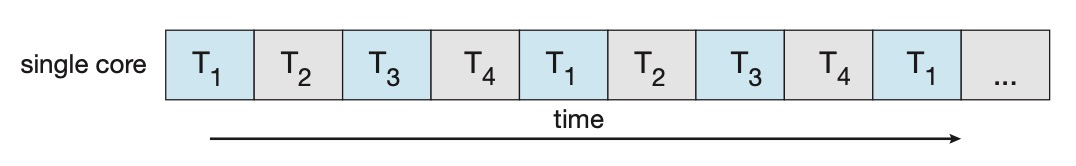
\includegraphics[width=0.65\linewidth]{assets/concorrenza.jpg}
    \caption{Concorrenza su un singolo processore}
\end{figure}

\subsection{Parallelismo}
Il parallelismo invece è la semplice esecuzione due o più task contemporaneamente. I due thread non devono necessariamente lavorare alla risoluzione dello stesso problema.
\begin{figure}[H]
    \centering
    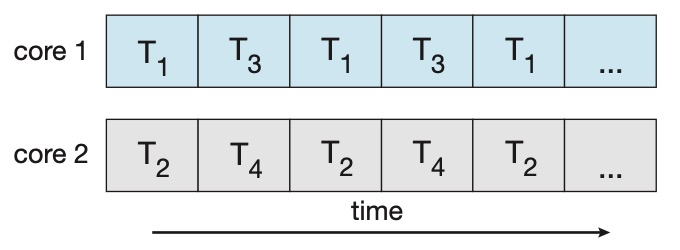
\includegraphics[width=0.45\linewidth]{assets/parallelismo.jpg}
    \caption{Parallelismo su due processori}
\end{figure}

\spacer
Il parallelismo può essere implementato in vari modi:
\begin{itemize}
    \item \textbf{Parallelismo dei dati:}

          La stessa operazione viene eseguita contemporaneamente su processori diversi su segmenti diversi dei dati. (es. per analizzare 10 ore di registrazione, divido in elementi da 1 ora ciascuno)

    \item \textbf{Parallelismo delle task:}

          Significa distribuire i threads tra più processori, ogni thread esegue un'operazione differente. I thread possono lavorare sugli stessi dati, ma non è necessario.
\end{itemize}

\begin{figure}[H]
    \centering
    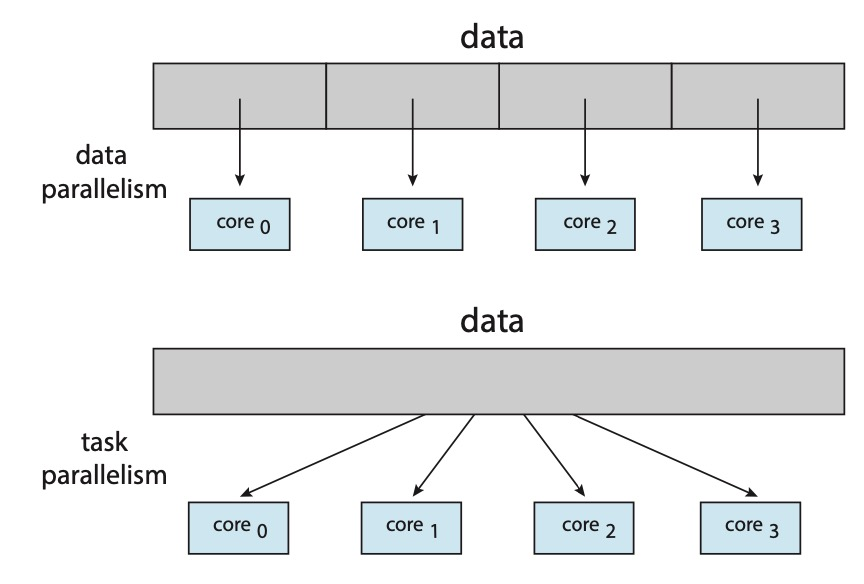
\includegraphics[width=0.45\linewidth]{assets/data-task-parallelism.jpg}
\end{figure}

\section{Sistemi di Processi}
È spesso conveniente scomporre un processo in $n$ sottoprocessi dando vita ad un sistema di processi, questo può permetterci di parallelizzare le operazioni pur rispettando l'ordine di esecuzione.

\begin{note}
    Possiamo utilizzare un grafo per rappresentare le relazioni di precedenza tra i processi, i nodi del grafo sono i sottoprocessi e un arco rappresenta una relazione di precedenza.
\end{note}

\subsubsection*{Esempio 4.1.}
Vogliamo risolvere l'equazione $f = (a + b) \cdot (c + d) + e$, possiamo risolverlo:
\begin{figure}[H]
    \centering
    \begin{minipage}{0.45\textwidth}
        \centering
        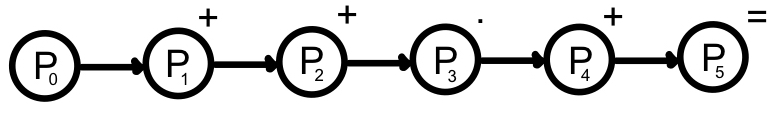
\includegraphics[width=\linewidth]{assets/math-sequenziale.jpeg}
        \caption{In modo sequenziale}
    \end{minipage}
    \hfill
    \begin{minipage}{0.35\textwidth}
        \centering
        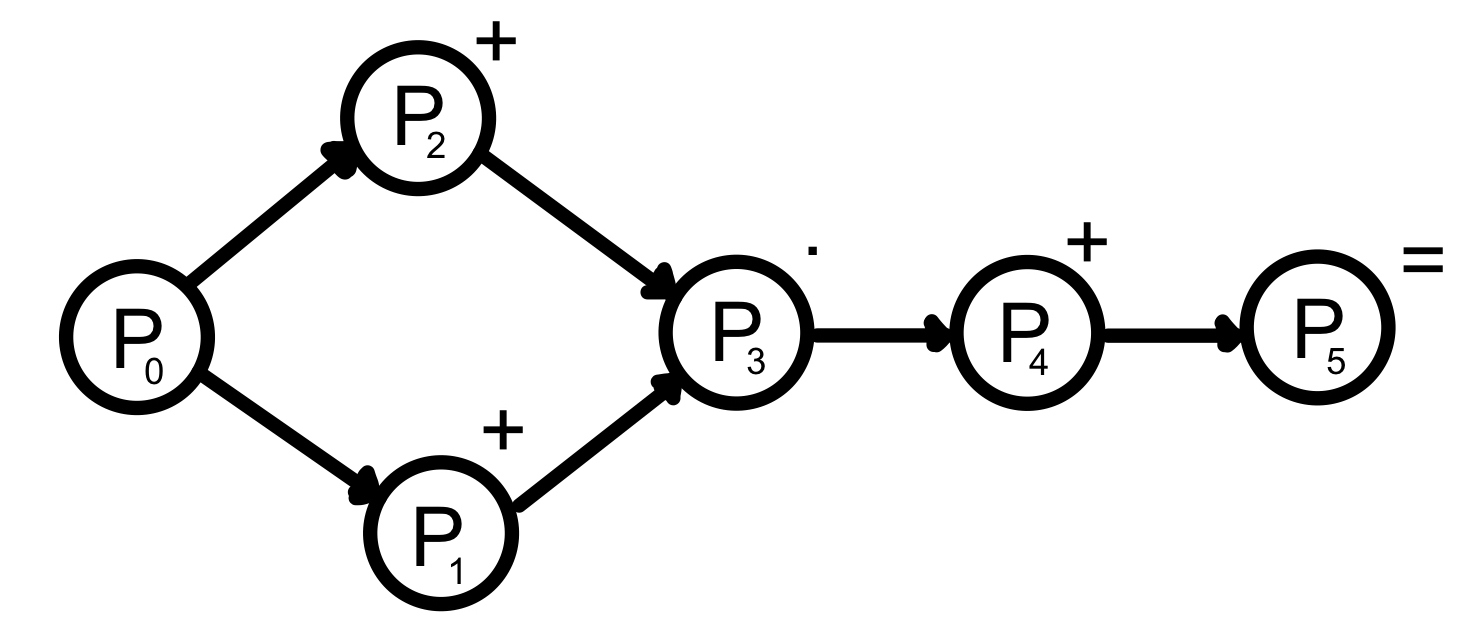
\includegraphics[width=\linewidth]{assets/math-parallelo.jpeg}
        \caption{In parallelo}
    \end{minipage}
\end{figure}

\subsubsection*{Esempio 4.2.}
Conoscendo i tempi di esecuzione di ogni singolo processo possiamo anche calcolare la quantità di tempo che viene risparmiata parallelizzando l'operazione.

\begin{figure}[H]
    \centering
    \begin{minipage}{0.45\textwidth}
        \centering
        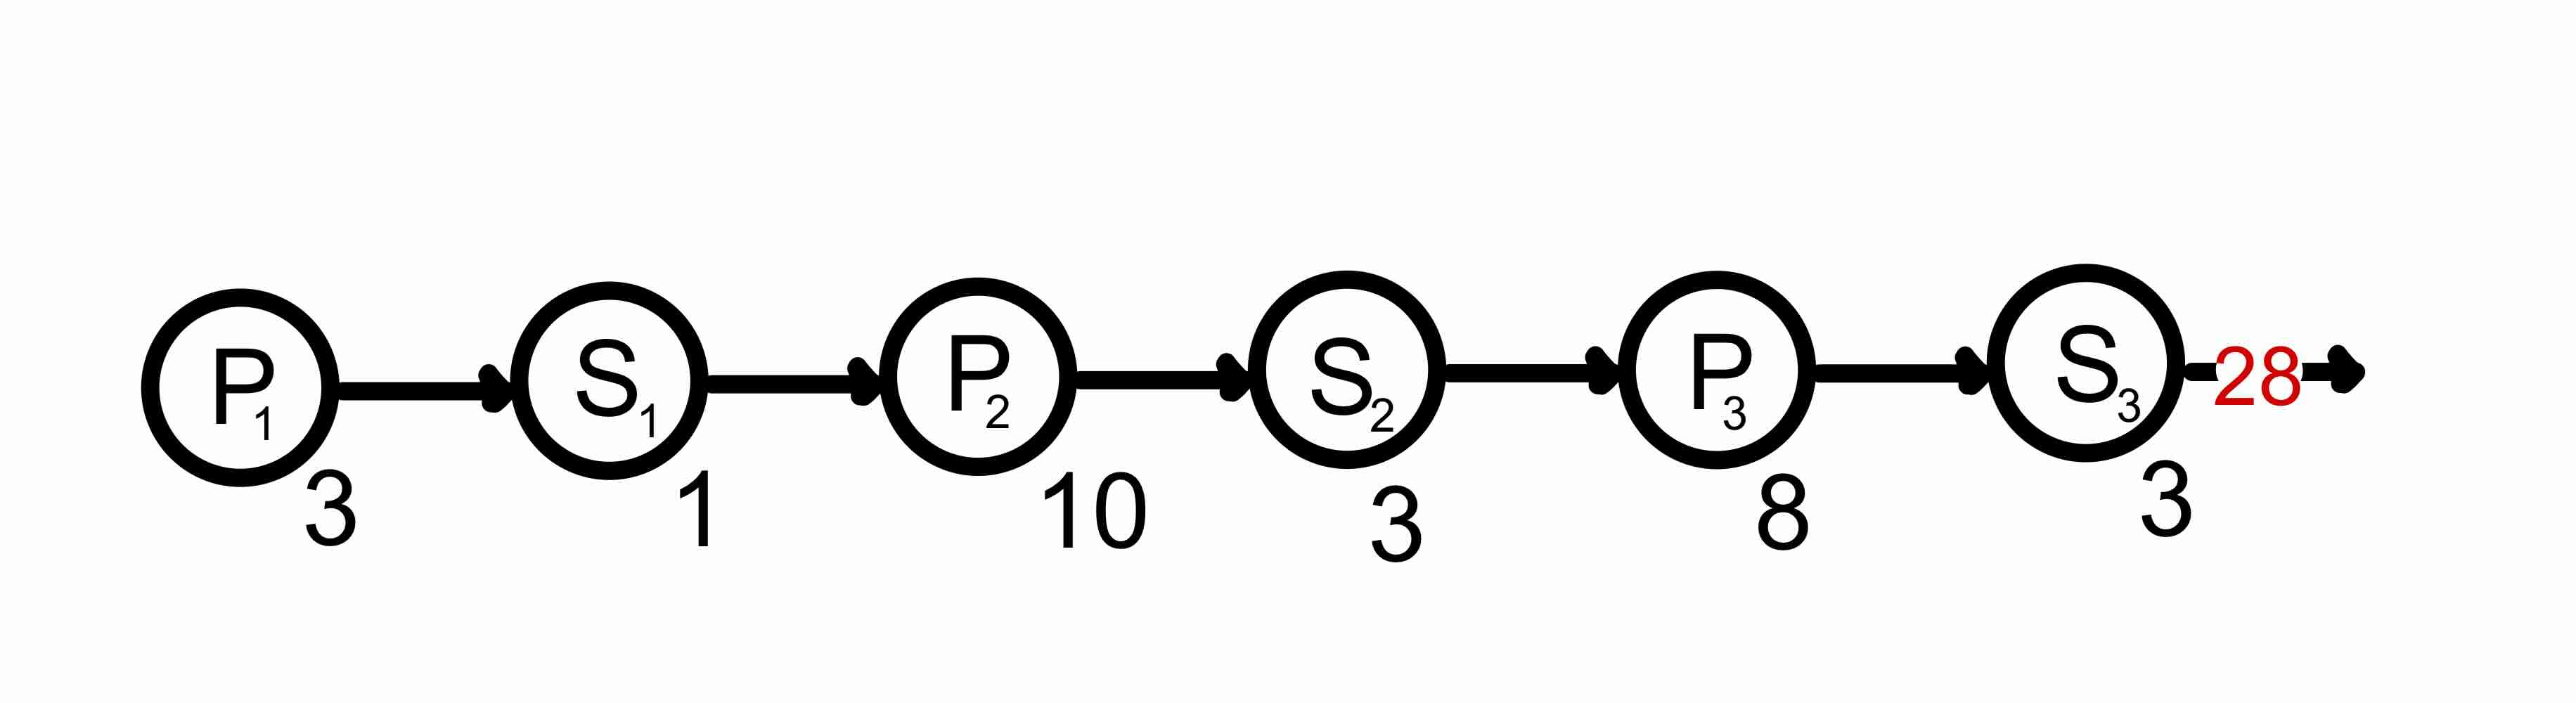
\includegraphics[width=\linewidth]{assets/threads-sequenziale.jpeg}
    \end{minipage}
    \hfill
    \begin{minipage}{0.35\textwidth}
        \centering
        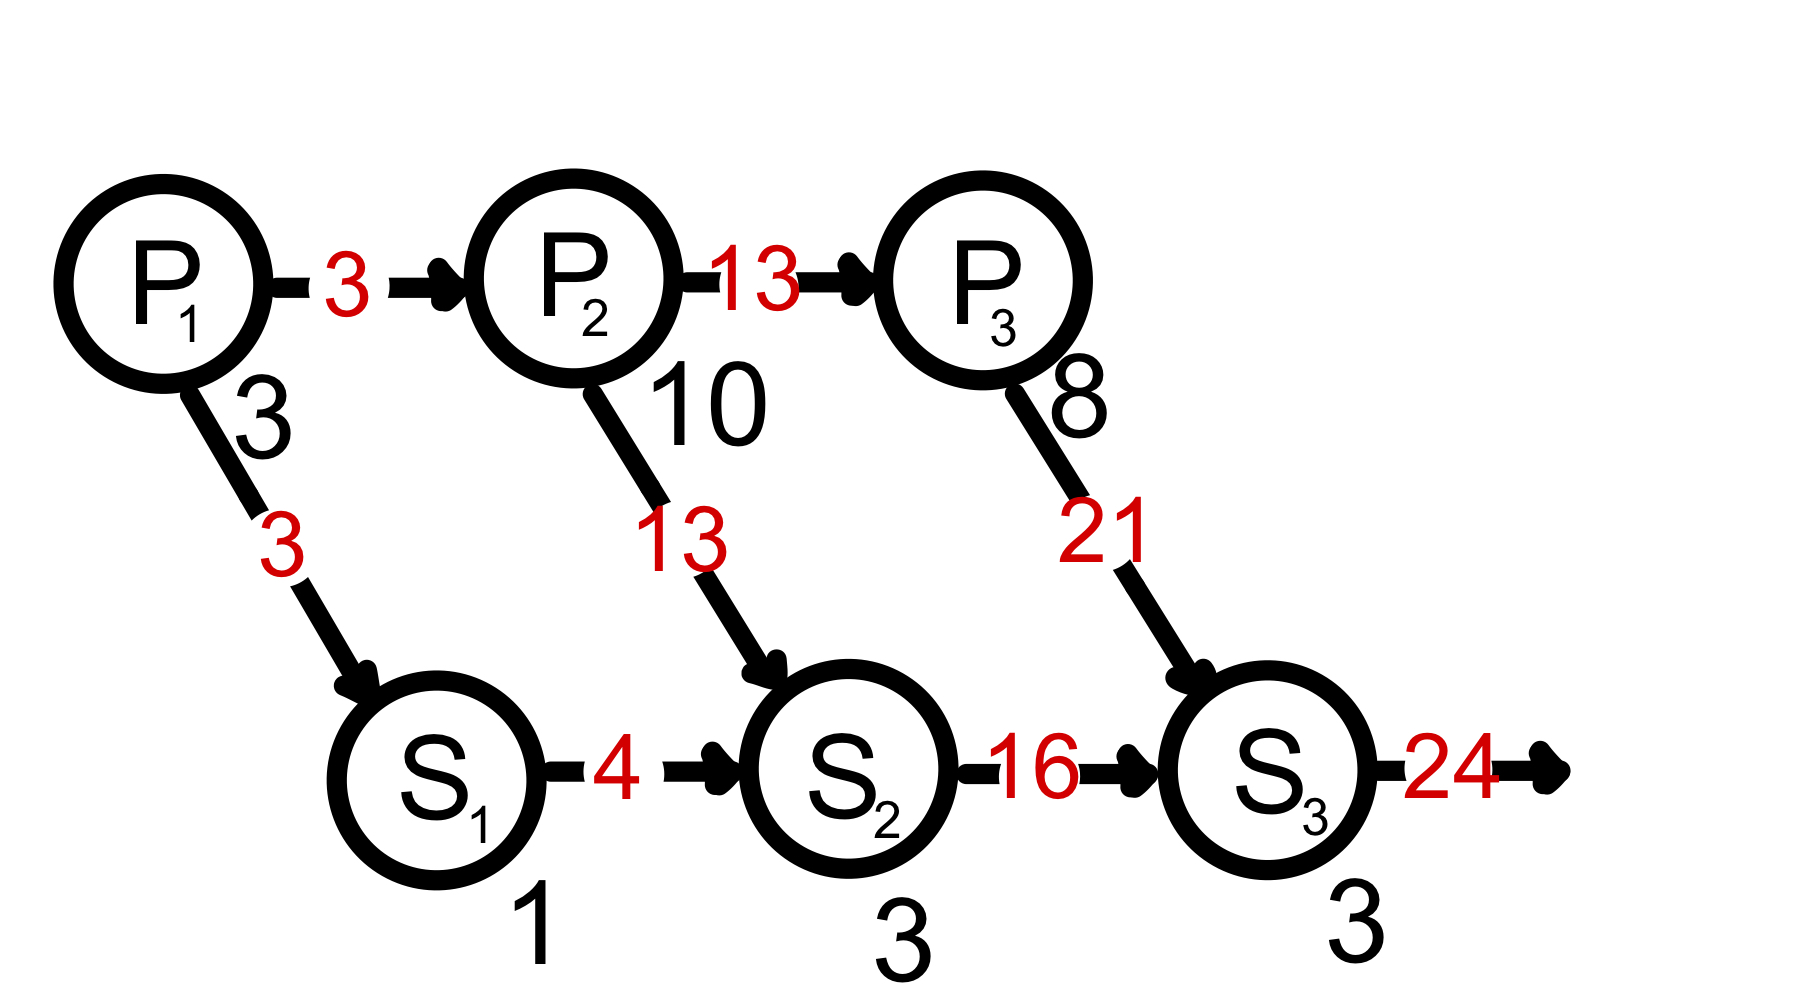
\includegraphics[width=\linewidth]{assets/threads-parallelo.jpeg}
    \end{minipage}
    \caption{Aumento di efficienza ottenuto parallelizzando il processo}
\end{figure}

\subsection{Sistemi Chiusi e Aperti}

Un sistema si definisce \textbf{chiuso} se esiste un singolo processo iniziale e un singolo processo finale.

Il sistema è \textbf{aperto} se non è chiuso.

\spacer

Due sistemi di processi possono essere combinati in \textbf{serie} o in \textbf{parallelo}.

\begin{figure}[H]
    \centering
    \begin{minipage}{0.45\textwidth}
        \centering
        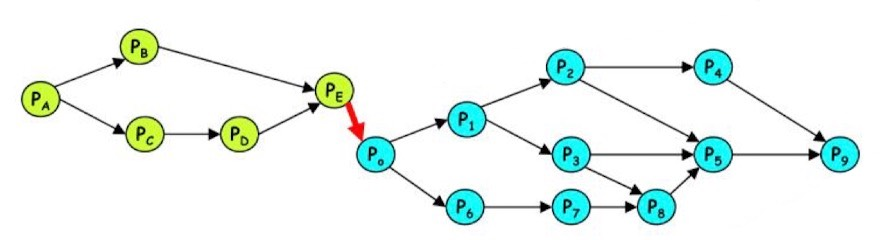
\includegraphics[width=\linewidth]{assets/sistema-serie.jpg}
    \end{minipage}
    \hfill
    \begin{minipage}{0.45\textwidth}
        \centering
        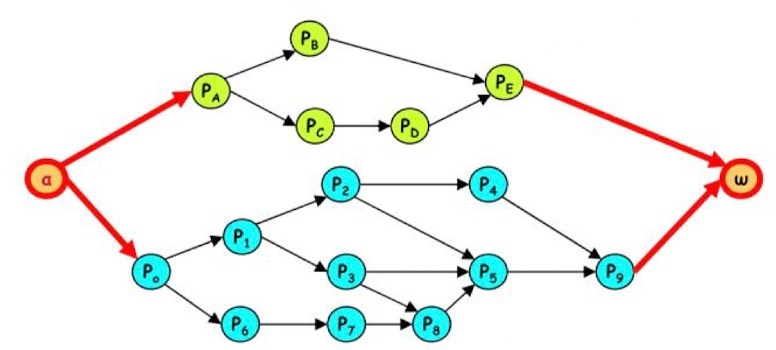
\includegraphics[width=\linewidth]{assets/sistema-parallelo.jpg}
    \end{minipage}
\end{figure}

\begin{note}
    I grafi ci permettono di trovare anche il \textbf{massimo grado di parallelismo} che un sistema raggiunge, si può trovare osservando il numero di processi nella stessa colonna.

    Nel caso rappresentato qui sopra ci sono al massimo 3 processi ponendo i sistemi in serie e 5 processi ponendo i sistemi in parallelo.
\end{note}

\subsection{Determinatezza}

Un sistema si dice \textbf{determinato} se le diverse velocità dei processi e l'ordine di esecuzione dei processi non influenzano il risultato.
Altrimenti si dice che il sistema è \textbf{indeterminato}.

\subsection{Inferenza}
\begin{note}
    Possiamo associare ad ogni processo un \textbf{dominio} contenente i dati su cui esso lavora e un \textbf{codominio} che contiene i risultati del processo.

    La \textbf{funzione mappa} trasforma elementi del dominio in elementi del codominio.
\end{note}

Due processi si dicono \textbf{non inferenti} se almeno una delle due osservazioni è corretta:
\begin{sitemize}
    \item Uno è il successore all'altro
    \item Non si intersecano i condomini e neppure i domini con i condomini.
\end{sitemize}

\subsubsection*{Proprietà}
\begin{sitemize}
    \item Condizione necessaria e sufficiente affinché un sistema sia \textbf{determinato} è che sia composto da processi \textbf{non inferenti}.
    \item Due sistemi sono \textbf{equivalenti} se sono costituiti dallo \textit{stesso insieme di processi}, sono \textit{determinati} e partendo dallo \textit{stesso input} producono lo \textit{stesso output}.
\end{sitemize}

\section{Risorse}
Diciamo \textbf{Risorsa} un'entità astratta, necessaria ad un processo per svolgere il proprio lavoro. Quando la risorsa non è disponibile il processo dovrà attendere per utilizzarla.

\spacer
Alcune risorse che sono \textbf{condivisibili} e possono essere usate da più processi in parallelo. Mentre alcune risorse possono essere usate da un solo processo allo stesso tempo.

\spacer
Un'altra classificazione delle risorse separa quelle non consumabili (es. un core), mentre altre sono \textbf{consumabili} (es. un dispositivo a batteria).

\spacer
Utilizziamo il termine \textbf{preemption} per definire la rimozione forzata di una risorsa ad un processo.

\subsection{Grafico dei Processi}

\begin{figure}[H]
    \centering
    \begin{minipage}{0.45\textwidth}
        \begin{tikzpicture}[scale=2.5]
            % assi
            \draw[->] (-0.1,0) -- (1.2,0) node[right] {$A$};
            \draw[->] (0,-0.1) -- (0,1.2) node[above] {$B$};

            % grafico
            \draw[smooth, line width=1.5pt] (0, 0) -- (0.2, 0);
            \draw[smooth, line width=1.5pt] (0.2, 0) -- (0.2, 0.1);
            \draw[smooth, line width=1.5pt] (0.2, 0.1) -- (0.4, 0.1);
            \draw[smooth, line width=1.5pt, red!60!gray] (0.4, 0.1) -- (0.4, 0.3);
            \draw[smooth, line width=1.5pt, green!60!gray] (0.4, 0.3) -- (0.7, 0.3);
            \draw[smooth, line width=1.5pt] (0.7, 0.3) -- (0.7, 0.4);
            \draw[smooth, line width=1.5pt] (0.7, 0.4) -- (0.9, 0.4);
            \draw[smooth, line width=1.5pt] (0.9, 0.4) -- (0.9, 0.7);
            \draw[smooth, line width=1.5pt] (0.9, 0.7) -- (1, 0.7);
            \draw[smooth, line width=1.5pt] (1, 0.7) -- (1, 1);

            \draw[smooth, line width=1.5pt] (0, 0.3) -- (0, 0.5) node[left] {$R_1$};
            \draw[smooth, line width=1.5pt] (0, 0.5) -- (0, 0.7);
            \draw[smooth, line width=1.5pt] (0.5, 0) -- (0.7, 0) node[below] {$R_2$};
            \draw[smooth, line width=1.5pt] (0.7, 0) -- (0.9, 0);
        \end{tikzpicture}

        In questo caso i due processi A e B si alternano. Nel tratto rosso viene eseguito il processo B, mentre A è in attesa. Nel tratto verde accade l'opposto, il processo B che attende in favore di A.

        Le risorse $R_1$ e $R_2$ sono risorse non condivisibili, A usa $R_1$ e B $R_2$.

    \end{minipage}
    \hfill
    \begin{minipage}{0.45\textwidth}
        \begin{tikzpicture}[scale=2.5]
            % assi
            \draw[->] (-0.1,0) -- (1.2,0) node[right] {$A$};
            \draw[->] (0,-0.1) -- (0,1.2) node[above] {$B$};

            \draw[smooth, line width=1.5pt] (0, 0.3) -- (0, 0.5) node[left] {$R_1$};
            \draw[smooth, line width=1.5pt] (0, 0.5) -- (0, 0.7);
            \draw[smooth, line width=1.5pt] (0.5, 0) -- (0.7, 0) node[below] {$R_1$};
            \draw[smooth, line width=1.5pt] (0.7, 0) -- (0.9, 0);


            \draw[dashed] (0, 0.3) -- (0.5, 0.3);
            \draw[dashed] (0, 0.7) -- (0.9, 0.7);

            \draw[dashed] (0.5, 0) -- (0.5, 0.3);
            \draw[dashed] (0.9, 0) -- (0.9, 0.7);

            \draw[fill=gray!30, draw=none] (0.5,0.3) rectangle (0.9, 0.7);

            % grafico
            \draw[smooth, line width=1.5pt] (0, 0) -- (0.2, 0);
            \draw[smooth, line width=1.5pt] (0.2, 0) -- (0.2, 0.1);
            \draw[smooth, line width=1.5pt] (0.2, 0.1) -- (0.4, 0.1);
            \draw[smooth, line width=1.5pt] (0.4, 0.1) -- (0.4, 0.2);
            \draw[smooth, line width=1.5pt] (0.4, 0.2) -- (0.9, 0.2);
            \draw[smooth, line width=1.5pt] (0.9, 0.2) -- (0.9, 0.7);
            \draw[smooth, line width=1.5pt] (0.9, 0.7) -- (1, 0.7);
            \draw[smooth, line width=1.5pt] (1, 0.7) -- (1, 1);

            \draw[smooth, line width=1.5pt, green!30!gray] (0, 0) -- (0, 0.2);
            \draw[smooth, line width=1.5pt, green!30!gray] (0, 0.2) -- (0.3, 0.2);
            \draw[smooth, line width=1.5pt, green!30!gray] (0.3, 0.2) -- (0.3, 0.7);
            \draw[smooth, line width=1.5pt, green!30!gray] (0.3, 0.7) -- (0.4, 0.7);
            \draw[smooth, line width=1.5pt, green!30!gray] (0.4, 0.7) -- (0.4, 0.8);
            \draw[smooth, line width=1.5pt, green!30!gray] (0.4, 0.8) -- (0.9, 0.8);
            \draw[smooth, line width=1.5pt, green!30!gray] (0.9, 0.8) -- (0.9, 1);
            \draw[smooth, line width=1.5pt, green!30!gray] (0.9, 1) -- (1, 1);
        \end{tikzpicture}

        In questo caso invece i due processi devono condividere la stessa risorsa $R_1$, questo significa che il grafico non può mai entrare nell'area grigia.

        I due percorsi, nero e verde, sono entrambi validi per l'esecuzione dei due processi, entrambi passano al di fuori dell'area vietata.

    \end{minipage}
\end{figure}

\section{Deadlock}
Quando due processi richiedono la stessa risorsa non condivisibile, uno dei due attende l'altro.

\spacer
In alcuni casi però si può arrivare ad una situazione più complicata, ovvero quando due o più processi si attendono a vicenda, questo viene detto \textbf{deadlock} o \textbf{stallo}.

\spacer
Le condizioni necessarie (ma non sufficienti) per il verificarsi di un \textbf{deadlock}:
\begin{enumerate}
    \item Tutte le risorse devono essere non condivisibili.
    \item Il processo non ha un'unica operazione in cui richiede delle risorse.
    \item Al processo non può essere rimossa la risorsa, solo esso stesso può rilasciarla.
    \item L'attesa avviene in modo circolare, se ci sono $n$ processi, $P_1$ attende $P_2$, $\ldots$, $P_(n-1)$ attende $P_n$ e $P_n$ attende $P_1$.
\end{enumerate}

In questo caso ogni processo attende una risorsa che non verrà rilasciata, tutti attendono e nessuno può procedere.

\subsubsection*{Livelock}
Un sottoinsieme dei deadlock sono i livelock o stalli attivi, rappresenta una situazione dove i thread non sono effettivamente bloccati, ma effettivamente non progrediscono (es. due persone che si incontrano e si spostano ripetutamente da un lato all'altro del corridoio)

\subsection{Grafo delle Risorse}
Una visualizzazione utile per evidenziare possibili deadlock in fase di progettazione è il grafo delle risorse.

\spacer
I nodi del grafo rappresentano thread ($T_1, T_2, \ldots, T_n$) e risorse ($R_1, R_2, \ldots, R_n$), spesso vengono visualizzati in modo differente per distinguerli.

Diciamo \textit{arco di richiesta} $T_i -> R_j$ e un \textit{arco di assegnazione} $R_i -> T_j$

\spacer
A questo punto possiamo dire che se il grafo non contiene cicli chiusi allora non ci saranno deadlock. Quando invece il grafo contiene un ciclo e vi è una sola istanza per ogni risorsa allora ci sarà un deadlock, se almeno una risorsa ha più di un'istanza allora il deadlock è solamente possibile.

\begin{figure}[H]
    \centering
    \begin{minipage}{0.45\textwidth}
        \centering
        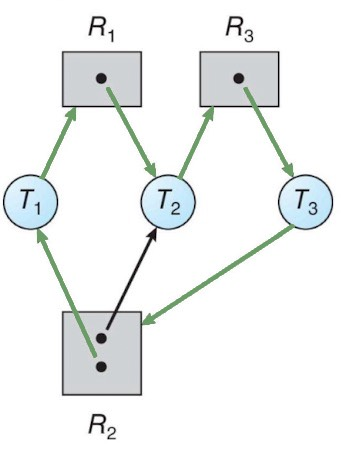
\includegraphics[width=0.65\linewidth]{assets/ciclo-deadlock.jpg}
        \caption{Situazione di deadlock}
    \end{minipage}
    \hfill
    \begin{minipage}{0.45\textwidth}
        \centering
        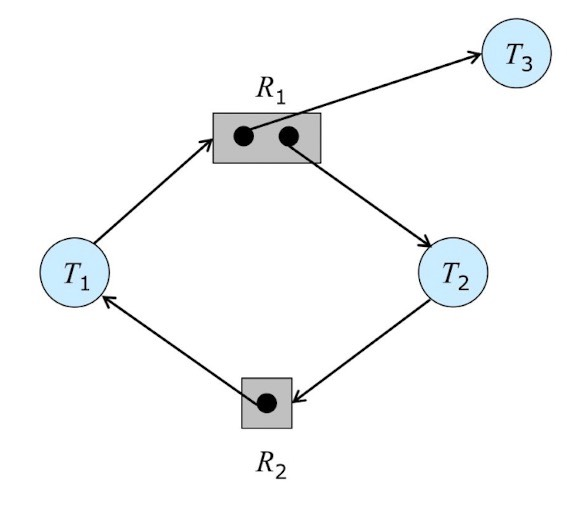
\includegraphics[width=0.9\linewidth]{assets/ciclo-no-deadlock.jpg}
        \caption{Situazione priva di deadlock}
    \end{minipage}
\end{figure}

\subsection{Prevenzione dei Deadlock}

\subsubsection{Allocazione globale}
Tutte le risorse richieste da un processo devono essere allocate prima che inizi l'esecuzione.

Questo garantisce l'assenza di deadlock, tuttavia è estremamente inefficiente reclamare tutte le risorse per tutto il periodo di esecuzione.

\subsubsection{Allocazione gerarchica}
Si assegna un ordine di importanza alle risorse, un processo può richiedere solo risorse più elevate di quelle che ha attualmente.
Se un processo necessita di una risorsa di priorità inferiore deve rilasciare quella attualmente in suo possesso per poi tornare a richiederla.

\begin{minipage}{0.45\textwidth}
    \begin{tikzpicture}[scale=2.5]
        % assi
        \draw[->] (-0.1,0) -- (1.2,0) node[right] {$A$};
        \draw[->] (0,-0.1) -- (0,1.2) node[above] {$B$};

        %R1
        \draw[smooth, line width=1.5pt] (0, 0.3) -- (0, 0.7) node[left] {$R_1$};
        \draw[smooth, line width=1.5pt] (0.5, 0) -- (0.9, 0) node[below] {$R_1$};


        \draw[dashed, gray] (0, 0.3) -- (0.5, 0.3);
        \draw[dashed, gray] (0, 0.7) -- (0.9, 0.7);

        \draw[dashed, gray] (0.5, 0) -- (0.5, 0.3);
        \draw[dashed, gray] (0.9, 0) -- (0.9, 0.7);

        %R2
        \draw[smooth, line width=1.5pt, red!50!gray] (0, 0.5) -- (0, 0.9) node[left] {$R_2$};
        \draw[smooth, line width=1.5pt, red!50!gray] (0.3, 0) -- (0.7, 0) node[below] {$R_2$};


        \draw[dashed, red!40!gray] (0, 0.5) -- (0.3, 0.5);
        \draw[dashed, red!40!gray] (0, 0.9) -- (0.7, 0.9);

        \draw[dashed, red!40!gray] (0.3, 0) -- (0.3, 0.5);
        \draw[dashed, red!40!gray] (0.7, 0) -- (0.7, 0.9);

        %squares
        \draw[fill=gray!30, draw=none] (0.5,0.3) rectangle (0.9, 0.7);
        \draw[fill=red!30, draw=none] (0.3,0.5) rectangle (0.7, 0.9);
        \draw[fill=white, draw=none] (0.3,0.45) rectangle (0.9, 0.5);

        % grafico
        \draw[smooth, line width=1.5pt] (0, 0) -- (0.2, 0);
        \draw[smooth, line width=1.5pt] (0.2, 0) -- (0.2, 0.1);
        \draw[smooth, line width=1.5pt] (0.2, 0.1) -- (0.4, 0.1);
        \draw[smooth, line width=1.5pt] (0.4, 0.1) -- (0.4, 0.45);
        \draw[smooth, line width=1.5pt] (0.4, 0.45) -- (0.9, 0.45);
        \draw[smooth, line width=1.5pt] (0.9, 0.45) -- (0.9, 0.7);
        \draw[smooth, line width=1.5pt] (0.9, 0.7) -- (1, 0.7);
        \draw[smooth, line width=1.5pt] (1, 0.7) -- (1, 1);
    \end{tikzpicture}
\end{minipage}

\subsubsection{Algoritmo del Banchiere}
Si impone che il thread $T_i$ inserisca nel grafo delle risorse tutti gli \textbf{archi di reclamo} a lui necessari prima di iniziare l'esecuzione.

Un arco di reclamo di un thread verso una risorsa indica al sistema che il thread utilizzerà in futuro quella risorsa. Un arco di reclamo diventa poi arco di richiesta in futuro.

\spacer
Definiamo \textbf{sequenza sicura} un ordinamento di n processi tali per lui le richieste di $P_i$ siano soddisfacibili dai processi $P_j$ con $j<i$

Uno \textbf{stato sicuro} è uno stato che contiene almeno una sequenza sicura.

\spacer
Per implementare l'algoritmo del banchiere vanno mantenute diverse strutture dati:
\begin{sitemize}
    \item Un \textbf{vettore $V$} che contiene il numero di istanze disponibili per ogni risorsa.
    \item Una \textbf{matrice $M$} che memorizza la massima quantità di istanze per ogni risorsa che viene usata dal thread.
    \item Una \textbf{matrice $R$} che memorizza le istanze per ogni risorsa attualmente allocate ad ogni thread.
    \item Una \textbf{matrice $N = M - R$}, che memorizza le risorse mancanti ad ogni thread.
\end{sitemize}

Tutte queste matrici devono essere aggiornate sia nei valori che nelle dimensioni.

\spacer
Per verificare che lo stato corrente sia sicuro deve essere possibile trovare almeno una sequenza di processi tale per cui sia possibile assegnare le risorse del vettore per completare ogni processo (le risorse necessarie al processo $i$ si trovano su $N[i]$)

\subsubsection{Algoritmo dello Struzzo}
L'algoritmo del banchiere deve essere eseguito frequentemente per poter rilevare i deadlock prima che si rivelino problematici, questo però richiede parecchie risorse del sistema.

\spacer
Per questo motivo molti sistemi \textit{consumer} \textbf{non} gestiscono i deadlock, essi avvengono in media una volta l'anno e in quel caso il sistema dovrà essere riavviato.

\subsection{Risoluzione di un Deadlock}
Una volta rilevato un deadlock per risolverlo ci sono due strategie spesso utilizzate.

\subsubsection{Terminazione dei Processi}
\begin{sitemize}
    \item Terminazione di tutti i processi che fanno parte del deadlock.

    Un sistema che risolve sicuramente il deadlock, ma viene anche ad un gran costo computazionale in quanto tutti i processi dovranno venir eseguiti da zero.

    \item Terminazione di un processo per volta finché il deadlock non viene rotto.
\end{sitemize}

\spacer
La scelta del processo da terminare è anch'essa gestita da un algoritmo che prende in considerare molti fattori, come la priorità del thread, il tempo di computazione trascorso, quantità di risorse che utilizza.


\subsubsection{Prelazione di Risorse}
Per risolvere il deadlock è anche possibile rimuovere risorse forzatamente ad uno o più processi.

Alcuni fattori da considerare quando si applica questa strategia sono:
\begin{sitemize}
    \item \textbf{Selezione della vittima}, è necessario scegliere un processo a cui rimuovere le risorse.
    \item \textbf{Rollback} dopo la rimozione della risorsa il thread non può continuare la sua esecuzione, è necessario tornare indietro a quando quella risorsa è stata acquisita.
    \item \textbf{Starvation} è importante non prelare le risorse sempre dallo stesso processo, altrimenti si potrebbe arrivare alla situazione in cui un processo non procede mai.
\end{sitemize}
\chapter{Sincronizzazione}

Quando due o più thread vengono eseguiti in parallelo devono essere sincronizzati correttamente per evitare l'insorgenza di race condition.

\section{Race Condition}
Quando più processi accedono in concorrenza e modificano i dati condivisi l'esito finale dell'esecuzione è indeterminato. Dipende dall'ordine in cui le loro istruzioni vengono eseguite.
Questa situazione viene chiamata \textbf{race condition} e va gestita per evitare di ottenere risultati erronei.

\subsubsection*{Esempio}

\spacer
\begin{minipage}{0.45\textwidth}
    \begin{minted}{java}
// Thread 1
for (int i = 0; i < 5; i++) {
    x++;
}
\end{minted}
\end{minipage}
\hfill
\begin{minipage}{0.45\textwidth}
    \begin{minted}{java}
// Thread 2
for (int j = 0; j < 5; j++) {
    x--;
}
\end{minted}
\end{minipage}
\spacer

In questo caso, se i due thread vengono eseguiti concorre mente, il valore finale di $x$ non è noto, potrebbe variare tra $-5$ e $+5$.

\subsubsection*{Operazioni Atomiche}

Per risolvere il problema della \textit{race condition} è necessario svolgere le operazioni di lettura e modifica delle variabili condivise senza interruzioni. Queste operazioni sono definite \textbf{atomiche}.

\section{Regioni Critiche}
Definiamo \textbf{Regioni Critiche} di un processo quelle regioni dove si accede ai dati in comune. Ci si deve quindi assicurare che solo un processo per volta possa entrare nella sua sezione critica.

\spacer
È importante gestire correttamente la sincronizzazione dei processi, ogni processo deve richiedere il permesso di entrare nella sezione critica e deve attendere che questo permesso gli sia garantito.

\spacer
Il protocollo di cooperazione tra processi deve garantire:
\begin{sitemize}
    \item \textbf{Mutua Esclusione:} un solo processo nella sezione critica per volta
    \item \textbf{Progresso:} Quando uno o più processi richiedono di entrare nella sezione critica la decisione deve essere fatta solo da processi che stanno già eseguendo la loro sezione critica o che potrebbero eseguirla in futuro. Ricordando sempre che la decisione non può essere rimandata indefinitamente.
    \item \textbf{Attesa Limitata:} Per evitare la \textit{starvation} è necessario limitare il tempo massimo di attesa.
\end{sitemize}

\subsubsection*{Kernel}
Anche le strutture dati del kernel, comprese quelle incaricate di gestire le risorse condivise, sono a loro volta suscettibili a race condition.

\spacer
È possibile risolvere questo problema utilizzando un kernel senza diritto di prelazione, quindi con processi che non escono dalla modalità kernel finché essi non si bloccano o restituiscono volontariamente il controllo alla CPU.

Questa è la soluzione utilizzata da Windows XP e Windows 2000, ma è particolarmente inefficiente per i sistemi multiprocessore e real-time.
Linux supporta la prelazione a partire dalla versione 2.6

\section{Lock}
In generale qualsiasi soluzione al problema della sezione critica utilizza il \textbf{lock}. Per accedere ad una sezione critica il processo deve acquisire un lock, che restituisce poi all'uscita dalla sezione critica.

\begin{minted}{java}
{
    //acquisisce il lock
    sezione critica
    //restituisce il lock
    sezione non critica
}
\end{minted}

\subsubsection*{Supporto Hardware}
Molte architetture forniscono il supporto hardware per implementare efficacemente i lock, inoltre alcune forniscono anche direttamente delle istruzioni atomiche.

\subsubsection*{Supporto Sistema Operativo}
Dato che le implementazioni hardware sono spesso inaccessibili ai programmatori, il sistema operativo fornisce degli strumenti per risolvere il problema.

Il più semplice è il \textbf{lock mutex}, permette di proteggere le sezioni critiche aggiungendo \texttt{acquire()} prima del segmento e \texttt{release()} al termine
\begin{minted}{java}
acquire() {
    while(!available) {}; // busy wait
    available = false;
}

release() {
    available = true;
}
\end{minted}

\section{Semafori}
I semafori sono uno strumento più avanzato per gestire la cooperazione di più processi.

\spacer
Un semaforo a N valori è una variabile $s$ intera e non negativa sulla quale si può effettuare:
\begin{sitemize}
    \item \textbf{Wait:} decrementa $s$ di 1 se $s>0$, altrimenti sospende il processo. (Oppure \textit{Probeer te verlagen}, P)
    \item \textbf{Signal:} Risveglia uno dei processi in attesa, se nessuno sta attendendo incrementa $s$ di 1. (Oppure \textit{Verhogen} V)
\end{sitemize}

\begin{minted}{java}
wait(S) {
    while(S <= 0) {}; // busy wait
    S--;
}

signal(S) {
    S++;
}
\end{minted}


Definiamo \textbf{Semaforo Contatore} il semaforo a valori in un dominio non limitato. Utile nel controllo di un numero finito di risorse, il semaforo viene inizializzato al numero di risorse disponibili.
\textbf{Semaforo Binario} assume solamente i valori 0 e 1, simile al lock mutex.

\subsection{Implementazione}
L'utilizzo del busy waiting rappresenta un problema per un processo multiprogrammato perché l'attesa spreca cicli di CPU che potrebbero essere usati da un'altro processo.

\spacer
Per risolvere questo problema si può associare ad ogni semaforo una coda di processi in attesa, spesso implementata tramite una queue (First In First Out).


\begin{minted}{java}
struct semaphore {
    int value;
    struct process* list; //puntatore al primo elemento della struttura dati
};

wait(semaphore *S) { 
    S->value--;
    if (S->value < 0) {
        add this process to S->list;
        sleep();
    }
}

signal(semaphore *S) { 
    S->value++;
    if (S->value <= 0) {
        remove a process P from S->list; 
        wakeup(P);
    }
}
\end{minted}

In questo caso $valore$ può essere $<0$, in quelle situazioni $|valore|$ è il numero di processi in attesa.

\subsection{Problemi di Utilizzo}
I semafori possono dare luogo a situazioni inaspettate che devono essere gestite attentamente.

\subsubsection*{Deadlock}
Si possono trovare situazioni in cui uno o più processi attendono risorse che possono essere liberate solo da uno degli altri processi in attesa.

\begin{minipage}{0.45\textwidth}
    \begin{minted}{java}
wait(S);
wait(Q);
...
signal(S);
signal(Q);
\end{minted}
\end{minipage}
\hfill
\begin{minipage}{0.45\textwidth}
    \begin{minted}{java}
wait(Q);
wait(S);
...
signal(Q);
signal(S);
\end{minted}
\end{minipage}

Linux fornisce uno strumento, lockdep, per rilevare i deadlock all'acquisizione di un lock.

\subsubsection*{Starvation}
Gestendo incorrettamente la lista associata al semaforo, per esempio utilizzando una struttura dati LIFO, è possibile che un processo attenda all'infinito nella coda senza mai venir rimosso.

\begin{figure}[H]
    \centering
    \includegraphics[width=0.5\linewidth]{assets/semaphore.jpg}
    \caption{Visualizzazione di un semaforo}
\end{figure}

\section{Monitor}
I semafori sono spesso utilizzare per sincronizzare l'utilizzo delle risorse, tuttavia il loro utilizzo incorretto può generare errori difficili da individuare.

\spacer
Un monitor è una struttura di più alto livello che contiene una serie di procedure e dei dati (condivisi tra i processi).
La caratteristica di un monitor è che al suo interno un solo processo per volta può essere attivo.

\begin{minted}{java}
monitor monitor_name {
    /* dichiarazioni delle variabili condivise */
    function P1 () {}
    function P2 () {}
    ...
    function PN () {}
}
\end{minted}

\subsection{Variabili Condition}
Le funzionalità appena descritte non sono sufficienti per modellare gran parte degli schemi di sincronizzazione.

Per questo vanno introdotte le variabili condition, da inserire tra le variabili condivise, sulle quali si possono effettuare solamente le operazioni di \texttt{wait()} e \texttt{signal()}.

Un processo può usare una variabile condition per attendere il verificarsi di una determinata condizione, uscendo dal monitor nell'attesa per lasciarlo libero ad altri processi.

\begin{figure}[H]
    \centering
    \includegraphics[width=0.6\linewidth]{assets/monitor.jpg}
    \caption{Monitor con variabili condition}
\end{figure}

\subsection{Gestione di signal}
Quando un processo $P$ invoca \texttt{signal()} su una risorsa che è attesa da un altro processo $Q$ si ottiene una situazione che può essere gestita in due modi:
\begin{sitemize}
    \item \textbf{Segnalare e attendere:} Il processo $P$, dopo la chiamata a \texttt{signal} esce dal monitor e lascia che $Q$ esegua la sua parte di codice.
    \item \textbf{Segnalare e procedere:} Il processo $P$ completa la sua esecuzione e poi $Q$ viene eseguito.
\end{sitemize}

\spacer
La seconda opzione, segnalare e procedere, sembra essere più ragionevole finché non si considera che la condizione che $P$ segnala potrebbe non essere più valida quando $Q$ arriva ad essere eseguito.

\section{Implementazione: Linux}
Prima della versione 2.6 (2004) Linux utilizzava un kernel senza diritto di prelazione. Per ottenere delle sezioni critiche venivano disabilitati momentaneamente gli interrupt.

\spacer
Ad oggi Linux fornisce diversi strumenti per la sincronizzazione:
\begin{itemize}
    \item \textbf{Lock Mutex:} Una variabile booleana che indica se il lock è disponibile, modificata tramite chiamate a sistema.
          \begin{minted}{cpp}
#include <pthread.h>
/* create and initialize the mutex lock */ 
pthread mutex t mutex;
pthread mutex init (&mutex, NULL);

pthread mutex lock (&mutex); /* acquire the mutex lock */ 
/* critical section */
pthread mutex unlock (&mutex); /* release the mutex lock */ 
    \end{minted}
    \item \textbf{Spinlock:} Un ciclo di busy waiting che verifica periodicamente se il lock è libero. È particolarmente inefficiente per i sistemi single core, in quanto altri processi non vengono eseguiti e quindi la risorsa attesa non viene sbloccata. Mentre può fornire alcuni vantaggi su sistemi multicore in quanto il processo non esce dall'esecuzione.
    \item \textbf{Semafori:} Ne esistono di due tipi, con e senza nome. I semafori con nome sono condivisi da tutti i processi imparentati, mentre quelli senza nome possono essere utilizzati solo nel contesto del processo.
          \begin{minted}{cpp}
#include <semaphore.h>
/* Create the semaphore and initialize it to 1 */
sem_t *sem;
sem = sem open ("SEM", O CREAT, 0666, 1);

sem_wait (sem); /* acquire the semaphore */
/* critical section */
sem-post (sem); /* release the semaphore */ 
            \end{minted}
    \item \textbf{Interi atomici:} Un tipo le cui operazioni sono tutte definite in modo atomico. Essi non risentono dell'overhead introdotto dai tradizionali meccanismi di lock.
          \begin{minted}{cpp}
atomic_t counter;
atomic_set (&counter, 5); /* counter = 5 */
atomic_add (10, &counter); /* counter = 15 */
atomic_sub (4, &counter); /* counter = 11 */
atomic_inc (&counter); /* counter = 12 */
int value = atomic_read (&counter); /* value = 12 */
    \end{minted}

    \item \textbf{Variabili condition:} Sono le variabili utilizzate per la realizzazione di monitor, forniscono un wait e un signal che gestiscono in autonomia un lock.

          Il wait acquisice periodicamente il lock, verifica la condition e poi libera il lock.

\end{itemize}


\chapter{Scheduling CPU}
I processi vengono sempre eseguiti finché non richiedono di attendere un'altra risorsa.
A questo punto un sistema semplice attende la risorsa, sprecando cicli della CPU, con la multiprogrammazione puntiamo a ridurre i cicli sprecati al minimo.

\section{CPU scheduler}
Abbiamo visto in 2.3.1 il lifecycle di un processo, lo scheduler della CPU deve prendere una decisione in queste situazioni:
\begin{enumerate}
    \item \textbf{Suspend:} Avviene principalmente come risultato di una richiesta di I/O, è quindi richiesto dal processo stesso.
    \item \textbf{Resign:} Il processo viene forzatamente interrotto dallo scheduler.
    \item \textbf{Resume:} La condizione attesa diventa vera e il processo è pronto ad utilizzare nuovamente risorse di sistema.
    \item \textbf{Termina}
\end{enumerate}

Uno scheduler che effettua delle decisioni solo nel caso 1 e 4 si dice \textbf{senza diritto di prelazione}, il processo quindi viene eseguito fino al termine o finché non restituisce volontariamente il controllo al sistema operativo.

Gli scheduler dei sistemi operativi moderni sono tutti \textbf{con diritto di prelazione}, effettuano quindi tutte e 4 le decisioni per portare a migliori prestazioni.

\spacer
I kernel con diritto di prelazione devono gestire anche tutte le situazioni critiche:
\begin{sitemize}
    \item Possibili \textbf{Race condition} quando avviene l'accesso a dati condivisi tra processi.
    \item La possibilità che anche i processi del kernel vengano prelati interrompendo così operazioni cruciali effettuate dal sistema.
\end{sitemize}

\subsection{Implementazione}
Il massimo utilizzo delle risorse si ottiene implementando lo scheduler in modo tale che ogni processo esegua continui cicli di CPU-I/O burst.

\begin{figure}[H]
    \centering
    \includegraphics[width=0.22\linewidth]{assets/CPU-IO-burst.jpg}
\end{figure}

Ogni algoritmo di scheduling ha diversi criteri che prova ad ottimizzare, alcuni di questi sono:
\begin{sitemize}
    \item \textbf{Utilizzo della CPU}
    \item \textbf{Throughput:} Numero di processi che completano la loro esecuzione nell'unità di tempo.
    \item \textbf{Tempo di turnaround:} Tempo impiegato per l'esecuzione di un determinato processo
    \item \textbf{Tempo di attesa} nella ready queue
    \item \textbf{Tempo di risposta:} il tempo che intercorre tra una richiesta e una risposta.
\end{sitemize}

\begin{figure}[H]
    \centering
    \includegraphics[width=0.5\linewidth]{assets/scheduler.jpg}
    \caption{Diagramma di scheduling}
\end{figure}

\subsection{Meccanismo di Interruzione}
Con \textbf{Meccanismo di Interruzione} intendiamo il meccanismo messo a disposizione dell'elaboratore per salvare lo stato del processo interrotto per poi trasferire il controllo ad una subroutine che gestisce l'interrupt.

\spacer
Il kernel del sistema è composto da 3 sezioni, il \textit{First Interrupt Handler (FLIH)}, il dispatcher e l'implementazione degli strumenti di sincronizzazione.

\subsubsection{First Interrupt Handler}
Il \textit{First Interrupt Handler (FLIH)} ha il compito di determinare l'origine dell'interrupt e attivare il segmento di codice che la gestisce.

\spacer
Nel caso di un sistema che implementa la multiprogrammazione ci possono essere più processi in attesa, è quindi necessario costruire una coda delle interruzioni.

La coda delle interruzioni funziona assieme a la coda dei processi pronti ad eseguire, quando un processo esce dalla coda delle interruzioni viene inserito tra gli altri processi pronti in attesa di risorse computazionali.

\begin{figure}[H]
    \centering
    \includegraphics[width=0.45\linewidth]{assets/process-lifecycle.jpeg}
\end{figure}

\subsubsection{Implementazione Strumenti di Sincronizzazione}
Le primitive wait e signal sono implementate dal kernel in quanto possono essere utilizzate da tutti i processi, wait deve poter avere accesso diretto al dispatcher per comunicarci.

\spacer
Ogni semaforo ha una coda, in genere FIFO, che contiene tutti i processi che si sono fermati sul semaforo.

\begin{note}
    Non tutti i semafori sono implementati tramite FIFO, essi in generale possono avere diverse implementazioni e organizzazione.
\end{note}

\subsection{Dispatcher}
Il dispatcher ha il compito di assegnare le risorse di computazione al processo selezionato dallo scheduler. Esso gestisce il context switch tra vari processi.

\begin{figure}[H]
    \centering
    \includegraphics[width=0.5\linewidth]{assets/dispatcher.jpg}
    \caption{Context switch $P_0 \rightarrow P_1 \rightarrow P_0$ }
\end{figure}

Definiamo \textbf{Latenza di dispatch} il tempo impiegato dal dispatcher per scambiare un processo con un'altro. Nello schema qui sopra è il periodo in cui entrambi i processi sono in \textit{idle}.

\subsection{Scheduler ad alto livello}
Il compito di attrubuire il livello di priorità dei processi non è compito del dispatcher, ma dello scheduler di alto livello.

È possibile utilizzare un heap, così da avere buone prestazioni di inserzione ($O(\log_2 n)$) e rendere banale l'estrazione del processo a priorità maggiore.

\section{Comunicazione tra Processi}
La comunicazione tra processi è necessaria in diverse situazioni e viene implementata mediante diverse tecniche:
\begin{sitemize}
    \item \textbf{Scambio di Messaggi:} Richiede un overhead da parte del sistema operativo, ma non presenta conflitti ed è di più semplice utilizzo.
    \item \textbf{Memoria Condivisa:} Richiede l'intervento del kernel solo nell'allocazione iniziale, tuttavia gli accessi successivi devono essere gestiti direttamente dai processi.
    \item \textbf{Pipes Ordinarie:} Permettono la comunicazione unidirezionale tra due processi (produttore-consumatore).
    \item \textbf{Pipes Nominate:} Permettono la comunicazione bidirezionale a molteplici processi, questo avviene grazie ad un file di tipo speciale. Sono supportate sia da Unix che da Windows.
\end{sitemize}
\section{Algoritmi di Scheduling}

\subsection{Selezione}
Prima di vendere alcuni degli algoritmi più utilizzati dai sistemi operativi moderni vediamo il metodo che viene utilizzato per confrontare e migliorare gli algoritmi.

\subsubsection{Modelli Deterministici}
Nella valutazione analitica, si seleziona un set predeterminato di processi, e si simulano più algoritmi calcolandone il tempo medio di attesa nei vari casi.

\spacer
È possibile utilizzare la \textbf{Formula di Little} per avvicinarsi di più alla realtà:
Sia $n$ la lunghezza media della coda, $W$ il tempo medio di attesa e $\lambda$ il numero di processi in arrivo per unità di tempo. Allora $n = W \cdot \lambda$.

\subsubsection{Simulazione}
La simulazione implica la creazione di un modello del sistema di calcolo e un processo di logging dei dati.

\subsection{Algoritmi Comuni}

\subsubsection{First Come First Serve}
Un semplice algoritmo che fornisce le risorse al primo processo che le richiedono. Il criterio poi segue l'implementazione della coda FIFO, quando le risorse si liberano vengono assegnate al primo processo della coda.

Questa strategia non è efficace per i computer consumer in quanto un processo molto lungo può fermare l'esecuzione di altri processi brevi che l'utente richiede con maggiore urgenza.

\subsubsection{Highest Priority/Shortest Job First}
Viene fornito un valore di priorità ad ogni processo, le risorse vengono assegnate al processo con la priorità più alta.

Questo algoritmo presenta spesso il problema della \textit{starvation} dove i processi a priorità bassa non vengono mai eseguiti, ma introducendo l'\textit{aging} la priorità di un processo aumenta all'aumentare del suo tempo di attesa.

\subsubsection{Round Robin o Scheduling Circolare}
A ciascun processo vengono assegnate le risorse per un periodo di tempo limitato, solitamente 10-100 ms (un periodo più breve ha troppo overhead di switching, con uno più grande si ottiene un algoritmo FIFO)

Questo algoritmo ha in media un tempo medio di attesa maggiore di un algoritmo basato sulla priorità, ma ha un miglior tempo di risposta, cosa importante nei sistemi consumer.

\begin{figure}[H]
    \centering
    \includegraphics[width=0.65\linewidth]{assets/round-robin.jpg}
    \caption{Esempio di esecuzione dell'algoritmo}
\end{figure}

\begin{note}
    Spesso negli esercizi capita che un nuovo processo venga inserito nella coda ready allo stesso momento in cui un processo termina il suo quanto di tempo. Si incorre quindi in una situazione dove non è chiaro quale dei due processi verrà inserito prima nella ready queue.

    In questo caso è possibile scegliere la soluzione che si preferisce, con l'unico limite di restare consistenti all'interno dell'esercizio.
\end{note}

\subsubsection{Highest Response Ratio}
Definiamo un valore da utilizzare come priorità, la priorità del processo $P_i$ sarà $p_i = \frac{a_i + e_i}{e_i}$

Dove $a_i$ è il tempo di attesa del processo nello stato ready e $e_i$ è il tempo di esecuzione stimato.

\spacer
Questo significa che i processi brevi avranno una priorità maggiore, ma implementa anche l'\textit{aging} per evitare la \textit{starvation}.

\subsubsection{Code Multiple}
Come spesso accade la migliore soluzione vede l'utilizzo di più algoritmi allo stesso tempo, è possibile infatti costruire più code, tutte con algoritmi di gestione diversi. Poi sarà sufficiente allocare una certa percentuale di risorse ad ognuna delle code.

\subsubsection{Esempio 1.}
Questa strategia si può ad esempio utilizzare per dividere i processi che eseguono in foregorund e quelli in background. La coda in foreground avrà maggiore disponibilità di risorse e sarà gestita in Round Robin per assicurarsi un ottima esperienza utente, quella background avrà meno risorse a disposizione e sarà gestita in FIFO.

\subsubsection{Esempio 2.}
Le code multiple si possono utilizzare anche per implementare l'aging, ad esempio possiamo implementare 3 code nel seguente modo:

La prima e la seconda in Round Robin a 8 ms ed a 16 ms e l'ultima in FIFO.
In questo modo i processi ricevono tutti rapidamente 8 e poi 16 ms di tempo di esecuzione, risolvendo così i processi semplici, mentre i processi più lunghi finiscono nella coda FIFO e verranno eseguiti quando possibile.

\begin{figure}[H]
    \centering
    \includegraphics[width=0.32\linewidth]{assets/code-multiple.jpg}
\end{figure}

\subsubsection{Scheduling con Priorità Proporzionale alla frequenza}
Un caso tipico industriale è quello in cui i processi devono essere eseguiti ad intervalli regolari. In questo caso è conveniente definire una priorità proporzionale alla frequenza. Quindi processi che utilizzano la CPU con più frequenza avranno priorità maggiore.

\spacer
Questo è un algoritmo ottimale, quindi se esso non riesce a pianificare l'esecuzione di una serie di processi rispettando i vincoli temporali allora nessun altro algoritmo ci riuscirà.
\begin{figure}[H]
    \centering
    \includegraphics[width=0.6\linewidth]{assets/coda-frequenza.jpg}
\end{figure}

È possibile calcolare a priori se i processi potranno essere eseguiti rispettando i vincoli tramite la seguente formula:
$$\sum_{i=1}^{m}\frac{C_i}{P_i} \le m\cdot(2^{\frac{1}{m}} - 1)$$
dove m è il numero di processi $P_i$ il periodo del processo $i$ e $C_i$ la sua durata.

\subsubsection{Earliest Deadline First}
Assegna le priorità dinamicamente a seconda delle scadenze. Ogni processo per poter essere eseguito deve annunciare la sua prossima scadenza allo scheduler, più questa scadenza si avvicina più la priorità del processo aumenta.

\subsubsection{Esempio}
Siano due processi $P_1$ e $P_2$ con periodo di 50 e 80 e con tempo di esecuzione di 25 e 35.
\begin{figure}[H]
    \centering
    \includegraphics[width=0.6\linewidth]{assets/edf.jpg}
\end{figure}
Dalla figura si può vedere come a t=100 il processo $P_1$ interrompe $P_2$ in quanto la sua deadline è a t=150 mentre $P_2$ ha come deadline t=160

\section{Scheduling Multiprocessore}
Il problema dello scheduling diventa più complesso quando nel sistema di calcolo sono presenti più processori.

\subsubsection*{Multielaborazione asimmetrica}
Un singolo processore, detto \textit{master server} ha il compito di gestire lo scheduling, l'I/O e le altre attività di sistema.

Questo riduce la necessità di condividere dati, un solo processore deve accedere alle strutture dati.

\subsubsection*{Multielaborazione simmetrica}
Quando più processori lavorano su strutture dati comuni è possibile incorrere in delle situazioni critiche, ad esempio quando due processori non possono eseguire lo stesso processo e nessun processo deve subire \textit{starvation}.

\spacer
Ci sono due filosofie sull'implementazione di questo tipo di scheduling:
\begin{itemize}
    \item Una coda per ogni processore, questo ha problemi quando è necessario ribilanciare le code in quanto l'overhead in questo caso è significativo.
          \begin{figure}[H]
              \centering
              \includegraphics[width=0.3\linewidth]{assets/one-queue-one-core.jpg}
          \end{figure}

          \begin{note}
              In questo caso risulta essere importante ripartire uniformemente il carico tra i vari processori.

              Un controllo delle lunghezze delle code avviene sia periodicamente sia quando un determinato processore diventa inattivo.
          \end{note}

    \item Una singola coda per tutti i processori, questo risolve il problema del bilanciamento, ma genera delle race condition nell'accesso alla struttura dati.
          \begin{figure}[H]
              \centering
              \includegraphics[width=0.3\linewidth]{assets/one-queue-many-core.jpg}
          \end{figure}
\end{itemize}

Esistono alcuni processi che hanno una predilezione per essere eseguiti sempre nello stesso core, questo permette loro di sfruttare al meglio la cache, ma non è sempre supportata dal sistema operativo.

\subsubsection*{Bilanciamento del Carico}
È il procedimento che permette di ripartire uniformemente il carico di lavoro tra più processori, può essere implementata in due modi:
\begin{sitemize}
    \item \textbf{Migrazione Guidata:} Un processo dedica controlla periodicamente il carico dei processori per correggere anticipamente gli equilibri
    \item \textbf{Migrazione Spontanea:} Un processore inattivo sottrae ad uno sovraccaricato un processo tra quelli in attesa.
\end{sitemize}

\subsection{Implementazioni}
\subsubsection{Linux}
Prima della versione 2.5 il kernel Linux implementava delle code multiple gestite perlopiù in Round Robin. La priorità viene calcolata periodicamente in base a quante risorse un processo ha consumato dall'ultimo controllo, minori sono le risorse utilizzate, maggiore sarà la priorità.

\spacer
Dalla versione 2.6.23 il kernel Linux implementa due code, \textit{default} e \textit{real-time}, con uno scheduler \textit{CFS (Completely Fair Scheduler)} che assegna ad ogni task una percentuale del tempo di CPU.

A ciascuna task viene associata una priorità (-20 a +19)

\spacer
Lo scheduler associa ad ogni task il suo tempo di esecuzione virtuale, una quantità che tiene conto sia del tempo di esecuzione che della priorità della task. Quindi una task a bassa priorità avrà un \texttt{vruntime} maggiore di una a priorità più alta, anche se sono state entrambe eseguite per lo stesso tempo.
Lo scheduler poi esegue la task con il valore \texttt{vruntime} più basso.

\spacer
Lo scheduler Linux è ottimizzato anche per sistemi NUMA, implementando delle strategie per ridurre al minimo il numero di migrazione dei processi da un processore all'altro.

\spacer
Le CPU Alder Lake causano non pochi problemi allo scheduler Linux < 5.16, infatti esso non si aspetta di vedere processori con livelli di prestazione diversi, ottimizzati per diverse situazioni.

\subsubsection{Windows 10}
Implementa livelli di priorità da 0 a 31, ognuno con la sua coda. Lo scheduler poi seleziona l'ultimo processo dalla coda a priorità più alta non vuota.

\spacer
I thread che hanno una priorità compresa tra 0 e 15 vengono gestiti dinamicamente, quando uno di essi viene portato in foreground, oppure riceve un input dall'utente, la sua priorità viene aumentata.

Inoltre la priorità dinamica viene diminuita di un livello ogni volta che il processo accede alle risorse della CPU, fino a tornare alla priorità base.

\subsubsection{Windows 11}
Windows 11 è stato scritto pensando alle nuove CPU intel, le quali hanno dei core ad alte prestazioni e degli altri ad alta efficienza.

Lo scheduler del sistema interagisce attivamente con un microcontrollore integrato nella CPU, chiamato \textit{Thread Director}.

Esso comunica al sistema operativo dei consigli sulla gestione dei processi processi prendendo in considerazione la situazione attuale del processore.

\spacer
Un'altra funzionalità introdotta da Windows 11 è il GPU accelerated scheduler, esso permette alla GPU di autogestire alcune task e la sua VRAM, alleggerendo il carico sulla CPU.

\subsubsection{Sistemi Real Time}
I sistemi operativi real time si dividono in:
\begin{sitemize}
    \item \textbf{Hard Real Time:} Richiedono il completamento di alcuni processi critici entro limiti specifici.
    \item \textbf{Soft Real Time:} Richiedono solo che ad alcuni processi venga fornita una priorità maggiore.
\end{sitemize}



\part{Gestione della Memoria}

\chapter{Gestione Memoria Principale}
Abbiamo già visto nei capitoli precedenti l'importanza della memoria principale nella gestione dei processi. Il sistema operativo ha il compito di gestirla in modo efficiente così da permettere l'esecuzione dei programmi.

\section{Introduzione}
Alla compilazione di un programma il compilatore genera un modulo oggetto dove tutti gli indirizzi sono in \textbf{riferimento} a quello dell'inizio del modulo. Questo significa che c'è libertà di inserire il processo in qualsiasi punto della memoria e ci sono quindi decisioni che il sistema operativo è responsabile di prendere.

\spacer
Per mantenere la sicurezza dei dati è importante che ogni processo possa accedere solamente ai dati ad esso assegnati, per questo motivo assegniamo ad ogni processo due indirizzi logici, uno base ed uno limite. Ora il processo può accedere solo agli indirizzi tali che $base \le indirizzo \le base+limite$.

\begin{figure}[H]
    \centering
    \includegraphics[width=0.3\linewidth]{assets/base-limit-memory.jpg}
\end{figure}

Nei sistemi moderni il processo può essere rilocato nella memoria a \textit{runtime}, questo grazie all'utilizzo della memoria virtuale. Questo ci permette di tradurre gli indirizzi fisici della memoria in indirizzi virtuali, non è quindi necessario allocare ad un programma un segmento contiguo di memoria, ma è possibile rendere contigui segmenti fisicamente lontani in memoria.

Questa traduzione avviene a livello hardware da parte della memory mapping and managment unit (MMU).

\begin{figure}[H]
    \centering
    \includegraphics[width=0.45\linewidth]{assets/MMU.jpg}
\end{figure}

\subsubsection*{File di Paging}
Una funzionalità introdotta da Windows XP, che estende la memoria RAM del sistema con un file presente in memoria secondaria, delle stesse dimensioni.

\subsection{Frammentazione}
L'allocazione e la rimozione della memoria comporta la frammentazione della memoria.
\begin{sitemize}
    \item La \textbf{frammentazione interna}, quando la memoria allocata ad ogni programma è leggermente maggiore di quella richiesta.
    \item La \textbf{frammentazione esterna}, quando lo spazio per un nuovo processo è disponibile, ma non è contiguo, in questo caso può essere necessario rilocare dei processi per compattare lo spazio libero.
\end{sitemize}

\section{Paginazione}
La paginazione risolve il problema posto dalla frammentazione esterna consentendo la non contiguità degli indirizzi fisici, mantenendo invece la contiguità negli indirizzi logici.

\subsection{Implementazione}
Si divide la memoria fisica in blocchi di dimensione fissa, detti frame o pagine fisiche. Allo stesso modo si divide anche la memoria logica in blocchi della stessa dimensione.

La \textbf{tabella delle pagine}, tiene traccia delle relazioni tra memoria fisica e logica e tiene traccia delle pagine libere.

\spacer
Gli indirizzo logici generati dalla CPU vengono suddivisi in:
\begin{sitemize}
    \item \textbf{Numero di pagina:} indice che verrà usato nella tabella delle pagine.
    \item \textbf{Offset nella pagina:} definisce l'offset a partire dall'inizio della pagina
\end{sitemize}

\begin{figure}[H]
    \centering
    \includegraphics[width=0.35\linewidth]{assets/page-number-offset.jpg}
\end{figure}

Se lo spazio logico ha dimensione $2^m$ allora si hanno $2^{m-n}$ pagine di dimensione $2^n$. La scelta di m ed n detta anche la dimensione della tabella delle pagine.

\begin{figure}[H]
    \centering
    \includegraphics[width=0.48\linewidth]{assets/paginazione.jpg}
\end{figure}

\subsubsection*{Frammentazione}
Si ottiene della frammentazione interna quando un processo non occupa completamente un frame, ad esempio un processo di 72766 byte occupa 36 pagine da 2048 byte, ma l'ultima pagina viene riempita circa a metà.

\subsubsection*{Dimensioni dei frame}
Un'importante considerazione che deve essere fatta nell'architettura dell'elaboratore è la dimensione delle pagine.

Pagine più piccole permettono una minore frammentazione in quanto si possono meglio adattare alle dimensioni del programma, esse migliorano inoltre il principio di località.

Al contrario pagine più grandi riducono le dimensioni della page table e riducono il numero di page fault incontrati.

La soluzione adottata da molti sistemi operativi è quella di costruire pagine di diverse dimensioni così da potersi adattare ad ogni processo.

\subsubsection*{Pagine Bloccate}
In alcuni casi occorre mantenere delle pagine perennemente in memoria, come nel caso di operazioni di I/O tramite DMA, per questo motivo è possibile segnalare al pager delle pagine bloccate (\textit{pinned}) che non possono essere selezionate come vittime dall'algoritmo di sostituzione.

\subsection{Supporto Hardware}
Si utilizza una tabella delle pagine per ogni processo, essa risiede nella memoria principale e il processo ha un puntatore ad essa (PTBR) ed alla sua lunghezza (PTLR).

\spacer
Uno degli svantaggi di inserire la tabella delle pagine nella memoria principale è l'\textbf{aumento del tempo di accesso dati}, infatti per ogni richiesta devono essere fatte due richieste alla memoria, una alla tabella ad una all'indirizzo fisico.

\spacer
Una soluzione è il \textit{translation look-aside buffer (TLB)} che permette la ricerca in parallelo su una piccola tabella (64-1024 elementi). Essa può essere utilizzata come cache per la tabella delle pagine.

La TLB è più efficiente e sicura quando non viene condivisa tra più processi, ad ogni \textit{context switch} andrebbe fatto un \textit{flush} della memoria.
È possibile aggiungere un valore \textit{Address Space IDentifier (ASID)} che identifica il processo a cui appartiene l'associazione, questo permette di mantenere la TLB di un processo anche in un context switch.

\begin{figure}[H]
    \centering
    \includegraphics[width=0.5\linewidth]{assets/paginazione-tlb.jpg}
\end{figure}

\subsubsection{Page Fault}
Se un processo fa riferimento ad una pagina che al momento non è in memoria principale viene generato un \textbf{interrupt} di tipo page fault.

Il processo viene quindi sospeso finché il sistema operativo non carica la pagina mancante in memoria principale. Se la memoria è piena è necessario utilizzare un algoritmo di camnio pagina per scegliere quale pagina rimuovere.

\subsubsection{Protezione della Memoria}
Viene implementata grazie ad uno o più \textbf{bit di protezione} che determinano se una è possibile accedere una determinata pagina in lettura oppure lettura/scrittura.

\spacer
Inoltre viene aggiunto un \textbf{bit di validità}, esso permette di individuare le pagine che non appartengono agli indirizzi \textit{logici} del processo, questo viene poi segnalato all'utente tramite un'interrupt.

\subsection{Dimensioni della Tabella}
La tabella delle pagine può arrivare facilmente a dimensioni importanti, soprattutto quando se ne crea una per ogni processo, una rappresentazione naturale, ma inefficiente.

\subsubsection*{Tabella delle Pagine Invertita}
Una soluzione è costruire una tabella delle pagine invertita, la quale ha un elemento per ogni frame fisico e salva il frame logico e un identificatore del processo.


Questo riduce lo spazio totale usato dalle tabelle delle pagine ma incrementa il tempo di ricerca nella tabella.
Inoltre rende difficile la condivisione delle pagine fisiche tra processi.

\begin{figure}[H]
    \centering
    \includegraphics[width=0.45\linewidth]{assets/tabella-pagine-invertita.jpg}
\end{figure}

\subsubsection*{Paginazione Gerarchica}
L'idea con questa soluzione è quello di dividere lo spazio degli indirizzi logici in più tabelle delle pagine. Il caso più semplice è quello ottenuto utilizzando una paginazione a due livelli.

\begin{figure}[H]
    \centering
    \includegraphics[width=0.35\linewidth]{assets/paginazione-doppia.jpg}
\end{figure}

$p_1$ viene utilizzato per indicizzare la tabella delle tabelle, mentre $p_2$ per indicizzare la tabella delle pagine.

\begin{figure}[H]
    \centering
    \includegraphics[width=0.5\linewidth]{assets/paginazione-gerarchica.jpg}
\end{figure}

Per le architetture a 64 bit questo tipo di paginazione necessita di troppi livelli di paginazione, è quindi da considerarsi inadeguata.

\subsubsection*{Tabella delle Pagine Hash}
Comunemente utilizzato per architetture a 64 bit.

L'elemento che viene inserito nella funzione di hash è il numero della pagina virtuale. Gli elementi della tabella sono liste concatenate, questo per gestire le eventuali collisioni dovute alla funzione di hash.

\spacer

In particolare ciascun elemento della tabella è composto da:
\begin{sitemize}
    \item Numero della pagina virtuale
    \item Numero della pagina fisica
    \item Puntatore al frame successivo
\end{sitemize}

\begin{figure}[H]
    \centering
    \includegraphics[width=0.5\linewidth]{assets/hashed-page-table.jpg}
\end{figure}

\begin{note}
    Per gli spazi a 64 bit si utilizza una tabella delle pagine a gruppi, ovvero una tabella hash dove ogni elemento contiene riferimenti alle pagine fisiche corrispondenti ad un gruppo di pagine virtuali contigue.
\end{note}

\subsubsection*{Segmentazione}
Gestisce la memoria in segmenti di dimensione variabile, questo è più vicino a come l'utente immagina l'organizzazione della memoria. Ogni segmento è un'unità logica:
\begin{sitemize}
    \item Procedure e funzioni
    \item Variabili
    \item Oggetti
\end{sitemize}

Si ha quindi una \textbf{tabella dei segmenti} per ogni processo che mappa gli indirizzi logici in coppie base, limite.

\begin{figure}[H]
    \centering
    \includegraphics[width=0.48\linewidth]{assets/segmentazione.jpg}
\end{figure}

Due registri sono di particolare importanza in questo caso: STRB (\textit{Segment Table Base Register}) e STLR (\textit{Segment Table Length Register}).

\subsection{Implementazioni}
\subsubsection{Intel 32}
Il pentium supporta sia la segmentazione pura che la segmentazione mista a paginazione.

\begin{figure}[H]
    \centering
    \includegraphics[width=0.5\linewidth]{assets/architettura-memoria-pentium.jpg}
\end{figure}

I segmenti possono essere di dimensione variabile, fino a 64 Kbyte, e possono essere al massimo $16 K$ per processo, di questi al massimo $8 K$ possono essere privati (Informazioni nella \textit{Local Descriptor Table, LDT}) e altri $8 K$ condivisi (Informazioni nella \textit{Global Descriptor Table, GDT}).

Il selettore è di 16 bit, dove 13 bit rappresentano l'indice del segmento ($2^{13} = 8192$), 1 bit per indicare LDT o GDT e 2 bit di protezione.
Altri 16 bit sono di offset.

\begin{figure}[H]
    \centering
    \includegraphics[width=0.5\linewidth]{assets/pentium-segmentation.jpg}
\end{figure}

Nella tabella vengono salvate anche altre informazioni, come un bit per indicare se il segmento è in memoria principale e uno per indicare se è stato modificato.

L'indirizzo ottenuto dalla segmentazione può essere paginato. Le pagine per il pentium possono essere di 4MB (1 livello) o 4KB (2 livelli) e viene usata una paginazione a due livelli.

\begin{figure}[H]
    \centering
    \includegraphics[width=0.5\linewidth]{assets/intel32-3.jpg}
\end{figure}

La dimensione della descriptor table viene aumentata nel tempo, prima a 24 e poi a 32 bit

\subsubsection{PAE}
Anche detto \textbf{Page Address Extension}, permette di raggiungere i 64 Gbyte di memoria.

Le principali modifiche all'architettura sono due: Viene inserito un ulteriore livello di paginazione, una page directory pointer table di 4 elementi e gli elementi della descriptor table arrivano a 64 bit, di cui solo 36 vengono utilizzati, arrivando così ad indicizzare 64 Gbyte di memoria.

\spacer
Le singole applicazioni possono, in generale, accedere solamente a 4GB di memoria, ma esse possono essere inserite in 64 Gbyte di memoria.

Inoltre è possibile per le applicazioni utilizzare delle system call per spostare il proprio spazio di indicizzazione, permettendo così di accedere ad una maggiore quantità di memoria RAM.

\begin{figure}[H]
    \centering
    \includegraphics[width=0.75\linewidth]{assets/pae.jpeg}
\end{figure}

\subsubsection{Intel x86-64}
Nei sistemi a 64 bit in realtà non se ne usano così tanti ($2^{64} = 17,179,869,184$ GB), gli indici sono tutti a 48 bit, lasciando inutilizzati i primi 16 bit.

L'architettura supporta pagine da 4KB, 2MB, 1GB.

\begin{figure}[H]
    \centering
    \includegraphics[width=0.6\linewidth]{assets/x64-address.jpg}
\end{figure}

È possibile utilizzare la PAE anche qui con l'obiettivo di portare gli indirizzi fisici da 48 a 52 bit.

\subsubsection{ARMv8}
Anche i processori ARM lavorano su 64 bit ed anche loro utilizzano fino a 4 livelli di paging ottenendo così pagine da 4KB, 2MB, 1GB.

\begin{figure}[H]
    \centering
    \includegraphics[width=0.6\linewidth]{assets/arm-address.jpg}
\end{figure}

\section{Memoria Virtuale}
Abbiamo visto come la paginazione può permettere di condividere la memoria tra più processi, tuttavia è raro che un intero processo venga inserito nella memoria principale prima che venga eseguito.

Questo perché non tutte le sezioni del programma vengono eseguite allo stesso tempo, è quindi conveniente caricarle in modo dinamico.

\spacer
In questo modo le dimensioni totali del programma non sono più limitate dalle dimensioni della memoria fisica e viene lasciato più spazio nella memoria per la multiprogrammazione.

Inoltre l'utilizzo della memoria virtuale rende più semplice la condivisione di librerie o dati.

\subsection{Spazio degli Indirizzi Virtuali}
La memoria virtuale separa la memoria logica utilizzata dagli sviluppatori da quella fisica, rendendo così più semplice il lavoro del programmatore che non deve gestire manualmente le limitazioni fisiche della memoria principale.

\spacer

Nello spazio degli indirizzi virtuali i programmi sono allocati in modo contiguo, a partire da un certo indirizzo iniziale $0$ fino a quello finale $Max$.

Nella memoria fisica invece il programma può essere allocato in pagine sparse. La MMU si occupa della conversione degli indirizzi logici in fisici.

\spacer
Condividere librerie è ora estremamente semplice, basterà mappare le pagine logiche agli stessi frame fisici.

In questo modo entrambi i processi vedono gli indirizzi della libreria comune come propri, ma in realtà i dati non vengono duplicati.

\section{Pager}
Un vantaggio della memoria virtuale è quello di poter caricare in modo dinamico i frame fisici dalla memoria secondaria. Il modulo del sistema operativo che si occupa della paginazione su richiesta è il \textit{pager}.

\spacer
Il termine \textit{swapping} indica l'atto di inserire o rimuovere delle pagine dalla memoria.
Quando una pagina viene rimossa dalla memoria essa viene riportata in un dispositivo di memroia secondaria, all'interno di un file (Windows) o una partizione (linux)

\spacer
Spesso si utilizza uno swapper pigro, che carica le pagine in RAM solo quando esse vengono richieste.

\begin{note}
    Inoltre spesso si utilizza una partizione di swap sulla memoria secondaria per ampliare ulteriormente le dimensioni della memoria principale, essa permette di ottenere delle prestazioni migliori in quanto non incorre nella frammentazione dei dischi.
\end{note}

Per sapere quali pagine si trovano già in memoria e quali invece devono essere caricate il pager utilizza una tabella delle pagine, essa associa la memoria logica a quella fisica. Inoltre comprende un bit di validità che specifica se il frame si trova in memoria o meno.

\begin{figure}[H]
    \centering
    \includegraphics[width=0.45\linewidth]{assets/tabella-pagine.jpg}
\end{figure}

\subsection{Page Fault}

Quando il programma richiede un indirizzo appartenente ad una pagina non caricata in memoria causa una trap al sistema operativo, una \textit{page fault}.

A questo punto il sistema operativo consulta una sua tabella delle pagine e invia al programma un abort se l'indirizzo non è valido.

Se viene trovata la pagina nella memoria secondaria allora essa viene caricata nella RAM e l'esecuzione del programma può riprendere.

\begin{figure}[H]
    \centering
    \includegraphics[width=0.5\linewidth]{assets/gestione-page-fault.jpg}
\end{figure}

Se non sono disponibili dei frame liberi nella memoria principale sarà necessario rimuovere prima una pagina secondo un algoritmo di selezione.
Si ricerca un algoritmo che riduca al minimo il numero di page fault in quanto esse sono un fattore importante sulle prestazioni del sistema.

\spacer
Viene impiegato un bit di modifica, o \textit{dirty bit}, per ridurre l'overhead dei trasferimenti di pagine. Solo le pagine modificate vengono riscritte al disco, le altre possono essere semplicemente sovrascritte.

\subsubsection{Prestazioni}
Il tempo effettivo di accesso alla memoria (EAT) si può calcolare nel seguente modo:
$$EAT = (1 - p)\cdot \text{accesso alla memoria} + p \cdot \text{overhead page fault}$$

Dove p è la probabilità di ottenere un page fault.

\spacer
Assumendo dei valori realistici, il tempo di acccesso alla memoria è di circa 200ns, mentre l'overhead per un page fault 8ms.

Sotto queste ipotesi se si ha un page fault ogni 1000 accessi l'accesso alla memoria viene mediamente rallentato di un fattore di 40.

Per ottenere un fattore di rallentamento accettabile (<0.1) è necessario arrivare ad un page fault ogni 400,000 richieste.

\subsection{Prepaging}
Per ridurre il gran numero di page fault che avvengono all'avvio del processo si può utilizzare il prepaging, ovvero si possono copiare un certo numero di pagine in memoria prima dell'esecuzione del programma.

\spacer
Ad esempio, se un programma è stato sospeso per una richiesta I/O, quando esso riprende l'esecuzione è possibile riportare in memoria il suo ultimo working set.

\spacer
È importante bilanciare le prestazioni di questa operazione ed assicurarsi che il vantaggio in riduzione di page fault sia superiore al costo di prepaging.

\subsection{Algoritmi di Paging}
Il paging richiede diversi algoritmi per un funzionamento corretto, in particolare sono necessari per l'allocazione dei frame e per la sostituzione delle pagine.

\begin{note}
    Alcune pagine devono rimanere bloccate (pinned) in memoria, non possono essere selezionate come vittime dagli algoritmi.
\end{note}

Gli algoritmi vengono valutati su una particolare stringa di riferimenti in memoria, ovvero 7 0 1 2 0 3 0 4 2 3 0 3 0 3 2 1 2 0 1 7 0 1.

\subsubsection{Algoritmo Ottimo}
L'algoritmo ideale è quello che rimuove la pagina che non verrà utilizzata per il periodo di tempo più lungo, in questo caso sulla stringa l'algoritmo genera 9 page fault.

Tuttavia questo non è possibile saperlo senza conoscere il futuro, cosa che il sistema non è ovviamente in grado di fare.

\subsubsection{FIFO}
L'algoritmo più semplice è forse quello FIFO, possiamo creare una coda con tutte le pagine di memoria fisica e sostituendo la prima entrata.

\begin{figure}[H]
    \centering
    \includegraphics[width=0.5\linewidth]{assets/FIFO-paging-ex.jpg}
    \caption{Example when usign a 3 frame memory}
\end{figure}

\begin{note}
    Non sempre aumentare le dimensioni della memoria porta ad una riduzione del numero di page fault, questo fatto è noto come \textit{Anomalia di Belady}.

    In particolare usando una coda FIFO con string dei riferimenti 1 2 3 4 1 2 5 1 2 3 4 5
    \begin{figure}[H]
        \includegraphics[width=0.4\linewidth]{assets/anomalia-belady.jpeg}
    \end{figure}
\end{note}

\subsubsection{LRU}
L'algoritmo rimpiazza la pagina che non è stata utilizzata per più tempo, provando a prevedere il futuro conoscendo il passato.

Questo algoritmo genera 12 page fault sulla stringa di riferimento.

\spacer
LRU viene considerato un buon algoritmo per questa applicazione, tuttavia risulta esserne difficile l'implementazione. Ci sono diverse soluzioni per l'implementazione, ma tutte richiedono dell'hardware dedicato per renderle praticabili.

\subsubsection{LFU}
Least Frequently Used, si rimpiazza la pagina meno utilizzata.

\subsubsection{MFU}
Most Frequently Used, si basa sull'idea che la pagina utilizzata più di recente non deve essere ricopiata in memoria per essere rimpiazzata.

\subsubsection{Seconda Chance}
L'algoritmo si basa su un algoritmo FIFO, ma viene aggiunto un bit di riferimento ad ogni pagina.

Il bit di riferimento di tutte le pagine viene inizialmente impostato a 0, quando vengono utilizzate viene impostato ad 1.

\spacer
Quando è necessario sostituire una pagina si cerca nella coda FIFO, se si incontra uno 0 quella pagina verrà rimossa. Altrimenti se si incontra un 1 si dà alla pagina una seconda chance, impostando il bit a 0 e spostandosi oltre.

\begin{figure}[H]
    \centering
    \includegraphics[width=0.9\linewidth]{assets/algoritmo-seconda-chance.jpg}
\end{figure}

L'algoritmo può essere migliorato tenendo conto anche del bit di modifica, si consideri la coppia (bit di riferimento, bit di modifica).

La pagina migliore è quella con valore (0, 0), seguita da (0, 1) che ha il difetto di dover essere salvata sulla memoria secondaria.

\subsubsection{Pool di Frame Liberi}
L'algoritmo richiede che venga sempre mantenuto un certo numero di frame liberi in memoria. Questi vengono utilizzati da buffer, dopo la selezione del frame vittima il nuovo frame viene scritto in uno dei frame liberi e infine il frame vittima viene copiato in memoria secondaria.

\spacer
Un'altra ottimizzazione disponibile è quella di controllare la memoria secondaria e quando esso è inattivo utilizzarlo per copiare dei frame modificati, resettando il loro bit di modifica.

\subsection{Allocazione dei Frame}
Il numero minimo di pagine che viene allocato ad un processo è deciso dall'architettura, mentre il massimo è dettato dalla dimensione della memoria primaria.

\subsubsection*{Allocazione Uniforme}
Semplicemente divide lo spazio della memoria per i programmi in esecuzione, quindi se si hanno 100 frame e 5 processi ognuno otterrà 20 frame.

\subsubsection*{Allocazione Proporzionale}
Uno schema di allocazione proporzionale alla dimensione del processo, un processo con più frame riceverà più risorse.

\subsubsection*{Allocazione con Priorità}
Si impiega uno schema basato sulla priorità, questa stessa priorità viene utilizzata anche per la scelta dei frame da rimuovere, un processo a priorità maggiore rimuoverà frame di processi a priorità inferiore.

\subsubsection*{Allocazione locale e globale}
L'allocazione globale permette ai processi di prendere frame da qualsiasi altro processo in esecuzione, quella locale invece limita le scelte ai frame che appartengono già al processo.

\spacer
Nei sistemi moderni si preferisce l'allocazione globale in quanto spesso garantisce un numero minore di page fault.

\subsection{Mappatura di File}
La mappatura di file in memoria permette l'accesso in modo completamente simile a quanto si fa per qualsiasi altro dato, l'accesso iniziale avviene tramite un page fault grazie al quale viene copiata una pagina di dati alla memoria principale.

\spacer
Questo permette anche di condividere il file tra più programmi in modo semplice dato che si trova in memoria virtuale.

Purtroppo ci sono anche degli svantaggi, legati principalmente a mantenere l'integrità del file anche in presenza di concorrenza.
\spacer
Il file viene aggiornato effettivamente in memoria solo alla chiusura o quando il pager decide di resettare il bit di modifica.

\spacer
Tutti i moderni sistemi operativi supportano la mappatura di file in memoria principale, spesso tramite una chiamata di sistema (\texttt{mmap()}).
Alcuni sistemi utilizzano la mappatura di default, come Solaris, rimuovendo così l'overhead causato dalla system call.

\subsubsection{Mappatura dell'I/O}
È possibile condividere informazioni tra processo e dispositivo I/O grazie alla mappatura in memoria, ad esempio un processo può scrivere su degli indirizzi di memoria, dai quali la scheda video prenderà i dati da mostrare all'utente.

\subsubsection{Copy On Write}
Le pagine di memoria vengono condivise tra due o più processi, quando uno vuole scrivere su una pagina la copia prima in una nuova locazione di memoria e poi la modifica.

\begin{figure}[H]
    \centering
    \includegraphics[width=0.5\linewidth]{assets/copy-on-write.jpeg}
\end{figure}

\section{Trashing}
Definiamo trashing la situazione in cui un processo è costantemente occupato a spostare pagine dal disco al posto di utilizzare le risorse del processore.

\spacer
Possiamo dire che c'è un certo numero di processi oltre il quale la multiprogrammazione diventa uno spreco di risorse, in quanto viene perso troppo tempo in page fault.
\begin{figure}[H]
    \centering
    \includegraphics[width=0.4\linewidth]{assets/trashing.jpg}
\end{figure}

Vogliamo quindi trovare il massimo numero di processi che possiamo eseguire in multiprogrammazione senza incorrere nel \textit{trashing}, per decidere questo utilizziamo il modello di località.

Il modello afferma che un processo si sposta da una località ad un'altra durante la sua esecuzione, una località è un insieme di indirizzi che sono spesso utilizzati insieme.

\subsection{Working Set}
Possiamo approssimare la località di un processo guardando ai frame che esso ha utilizzato nelle ultime $\Delta$ chiamate alla memoria, chiamiamo il set dei frame usati dal processo $i$ nel periodo $\Delta$ \textit{Working Set ($WSS_i$)} .

\begin{note}
    $\Delta$ deve essere della giusta dimensione, troppo piccolo e non conterrà tutta la località, troppo grande e conterrà più località
\end{note}

Rappresentiamo il Working set con due numeri: $WS(t, \Delta)$ dove il primo è l'istante che stiamo analizzando, mentre il secondo la dimensione della località.

Otteniamo quindi $D = \sum_i WSS_i$, il numero totale di frame attualmente nella località dei processi in esecuzione, se questo numero supera il numero totale dei frame disponibili nella memoria principale si rischia di incorrere nel \textit{trashing}.

A questo punto è conveniente terminare alcuni processi o sottoporli a swapping.

\spacer
Il working set è un insieme in constante cambiamento, quindi per alleggerirne l'utilizzo è conveniente effettuare il controllo su un determinato periodo e salvare quali frame sono presenti in almeno un working set in un bit di stato (1 se presente, 0 se non presente).

Quando sarà necessario rimuovere un frame si cercherà quello con il maggior numero di 0 nei suoi bit di stato, ovvero quello che non appare nei working set da più tempo.

\subsection{Frequenza di Page Fault}
Un approccio più diretto è quello di stabilire una certa frequenza di page fault "accettabile" e aumentare o diminuire i frame di conseguenza.

\begin{figure}[H]
    \centering
    \includegraphics[width=0.5\linewidth]{assets/frequenza-page-fault.jpg}
\end{figure}

\subsection{Relazione tra Working Set e Frequenza di Page Fault}
Il cambiamento di località comporta un picco di page fault

\begin{figure}[H]
    \centering
    \includegraphics[width=0.5\linewidth]{assets/page-fault-working-set.jpeg}
\end{figure}

\section{Allocazione di Memoria al Kernel}
Il kernel utilizza della memoria separata da quella destinata agli utenti, questa memoria molto spesso non è soggetta a paginazione in quanto esso opera con oggetti di piccole dimensioni che sprecherebbero le pagine.

Inoltre alcune parti della memoria del kernel devono essere contigue per permettere a dispositivi I/O, che non hanno accesso alla memoria fisica, di scriverci.

\spacer
Vedremo ora due tecniche per gestire la memoria che viene riservata al kernel.

\subsection{Allocatore potenza 2}
Utilizza un segmento di memoria a dimensione fissa e fisicamente contigua, che viene allocato in blocchi di dimensione pari a potenze del 2.

\spacer
Quando viene richiesta una quantità di memoria essa viene arrotondata alla più piccola potenza che la contiene, se si richiede una quantità di memoria minore il segmento viene diviso a metà.

\begin{figure}[H]
    \centering
    \includegraphics[width=0.4\linewidth]{assets/allocatore-potenza-2.jpg}
\end{figure}

\subsection{Allocazione a Lastra}
Il kernel ha la necessità di allocare e distruggere oggetti frequentemente, per questo motivo è conveniente mantenere una cache per ogni tipo di oggetto così da rimuovere il costo di inizializzazione.

\spacer
Le cache contengono istanze della struttura dati del kernel a cui sono assegnate e vengono inserite in una lastra (\textit{slab}), dei segmenti di memoria fisicamente contigui.

\spacer
Quando il kernel richiede un nuovo oggetto esso viene preso da quelli segnati come liberi.

Se non dovessero essere disponibili oggetti liberi ne vengono allocati altri in una lastra vuota. Nel caso in cui non dovessero esserci lastre libere verrà allocato spazio per far crescere la cache di una lastra.

\begin{figure}[H]
    \centering
    \includegraphics[width=0.5\linewidth]{assets/allocatore-lastra.jpg}
\end{figure}

\section{Implementazioni}
\subsection{Linux}
Per quanto riguarda la \textbf{Memoria del Kernel} linux utilizza il sistema Buddy, un allocatore potenza di 2.
Invece per le strutture dati, a partire dal kernel 2.4, viene utilizzato l'allocatore SLOB o SLUB.
\begin{sitemize}
    \item \textbf{SLOB:} Utilizzato per sistemi con poca memoria, mantiene 3 liste, per oggetti grandi, medi e piccoli.
    \item \textbf{SLUB:} Allocatore a lastre ottimizzata per sistemi multicore.
\end{sitemize}

\spacer
Invece la \textbf{Memoria Utente} viene gestita tramite paginazione su richiesta.
La politica di sostituzione è detta Clock: vengono mantenute due liste, \texttt{active\_list} e \texttt{inactive\_list}, la prima che contiene le pagine in uso e la seconda contiene pagine non utilizzate di frequente che possono essere rimosse.

\spacer
Ogni pagina ha un bit di accesso.
\begin{sitemize}
    \item Quando una pagina viene \textbf{allocata} o \textbf{riferita} il bit viene impostato su 1 e viene inserita in coda a \texttt{active\_list}.
    \item La pagina utilizzata meno di recente si sposta in testa alla lista \texttt{active\_list}, dalla quale viene \textbf{spostata} verso la lista \texttt{inactive\_list} per mantenere le due liste bilanciate.
    \item Inoltre i bit di accesso vengono resettati periodicamente, riportando il sistema ad uno stato iniziale con tutti i processi in \texttt{inactive\_list}.
    \item Il deamon \texttt{kswapd} si risveglia periodicamente e se la memoria non è sufficiente \textbf{termina} dei programmi dalla \texttt{inactive\_list}.
\end{sitemize}

\subsection{Windows}
Per quanto riguarda la \textbf{Memoria del Kernel} Windows scrive i dati su un page file, ma quando questo non è possibile i dati vengono scritti su una pool di memoria non paginata. (ad es. quando Windows non può fare page fault perché sta gestendo un page fault.)

\spacer
Invece la \textbf{Memoria Utente} viene gestita tramite paginazione con clustering, quindi quando avviene un page fault viene caricato non solo la pagina richiesta, ma anche le pagine adiacenti.

Ad un processo viene assegnato una dimensione minima e massima del working set, il minimo è il numero di pagine garantite dal sistema operativo, il numero massimo è il limite oltre il quale il processo non può allocare.

Quando l'occupazione della memoria scende si effettua una riassegnazione dei working set aumentando i tetti massimi per processo.

\spacer
Windows fa inoltre uso di compressione delle pagine più vecchie, prima di ricorrere alla memoria virtuale. Quando poi i dati tornano ad essere utilizzati devono prima essere decompressi.


\chapter{File}

Il \textit{file} viene definito come uno spazio di indirizzi logici contigui. È quindi un insieme di informazioni registrate nella memoria secondaria con delle informazioni correlate.

\spacer
Per gli utenti il file è la più piccola porzione di memoria secondaria indicizzabile e rappresentano l'unico modo di scrivere delle informazioni nella memoria secondaria.

\section{Tipo di Dati Astratto}
Un file è un tipo di dati astratto su cui sono definite le operazioni di:
\begin{sitemize}
    \item \textbf{Creazione}

    Reperisce dello spazio per memorizzare il file nella memoria e crea un nuovo elemento nella directory.

    \item \textbf{Scrittura}

    Viene fatta una \textit{system call} che specifica il file su cui scrivere e i dati da scrivere.
    Il sistema operativo mantiene un puntatore di scrittura per continuare una scrittura sequenziale.

    \item \textbf{Lettura}

    \textit{system call} con riferimento al file e indirizzo di memoria principale su cui scrivere i dati. Anche in questo caso il sistema operativo mantiene un puntatore di lettura per le letture sequenziali.

    \item \textbf{Posizionamento del File}

    Riposiziona il puntatore di lettura/scrittura ad un diverso punto del file.

    \item \textbf{Cancellazione}

    Si rilascia lo spazio allocato al file e lo si rimuove dalla directory. (I bit non vengono azzerati quindi i dati del file possono essere ancora letti)

    \item \textbf{Troncamento}

    Elimina il contenuto del file, ma ne mantiene tutti gli attributi

    \item \textbf{Impostazione degli attributi}

    Reperimento/aggiornamento delle informazioni del file nel relativo elemento della directory
\end{sitemize}

Da queste operazioni elementari è possibile poi costruirne di più complesse facendone una combinazione.


\section{Implementazione}

\subsection{Attributi dei File}
\begin{sitemize}
    \item \textbf{Nome:} Identificativo del file per l'utente.
    \item \textbf{Identificativo:} Etichetta unica utilizzata dal file system.
    \item \textbf{Tipo:} Specifica il tipo dei dati contenuti nel file, ad esempio testi, immagini, video oppure programmi.
    \item \textbf{Locazione:} Puntatore alla posizione del file sul dispositivo di memoria secondaria.
    \item \textbf{Dimensione:} Attuale dimensione del file.
    \item \textbf{Protezione:} Parametri di controllo su lettura/scrittura/esecuzione del file.
    \item \textbf{Ora, data, identificazione dell'utente:} Informazioni utili alla protezione del file.
\end{sitemize}

\begin{note}
    Gli attributi estesi sono una serie di informazioni aggiuntive che possono essere associate ad un file, essi sono una serie di coppie nome-valore e possono essere definiti dall'utente.

    Non vegnono salvati nel file, ma vengono salvati separatamente e gestiti dal file system.
\end{note}

\subsection{Tipo del File}
Il tipo del file è un attributo che indica la struttura interna e permette al sistema operativo di gestire il file in modo corretto.

\spacer
Le estensioni possono essere specificate in vari modi:
\begin{sitemize}
    \item Meccanismo delle estensioni (Windows)
    \item Attributo nella directory (MacOS)
    \item Valore posto all'inizio del file (Unix)
\end{sitemize}

\begin{figure}[H]
    \centering
    \includegraphics[width=0.5\linewidth]{assets/tipi-file.jpg}
\end{figure}

\subsection{Struttura del File}
Strettamente collegato al tipo del file, il quale può suggerirci la sua struttura interna.
\begin{sitemize}
    \item Nessuna Struttura (sequenza di byte)
    \item Struttura a record semplice (Linee a lunghezza fissa/variabile simili alle tabelle sql)
    \item Struttura complessa (documento formattato o eseguibile rilocabile)
\end{sitemize}

\spacer
Spesso è inefficiente lasciare al sistema operativo il compito di gestire ogni tipo di file, è più conveniente che esso sappia gestire solo i tipi base (spesso solamente i file eseguibili) e il resto viene lasciato a programmi di sistema o di terze parti.

Unix e DOS implementano questa scelta, i file sono gestiti solamente come stringhe di byte.


\section{Apertura di un File}
Prima di un qualsiasi accesso ai dati del file occorre trovare l'indirizzo fisico dei dati, ovvero è necessario "aprire" il file.

Il sistema operativo tiene poi in memoria una tabella dei file aperti che permette di accedere rapidamente ai file in uso.

Le system call che gestiscono questa funzione sono:
\begin{sitemize}
    \item \textbf{open(F):} ricerca il file nella directory del disco e copia il puntatore ai dati nella tabella dei file.

    \item \textbf{close(F):} copia il contenuto residente nella memoria principale alla memoria secondaria e rimuove il file dalla tabella.
\end{sitemize}

\subsection{Sistemi multiprogrammati}
Nei sistemi multiprogrammati la gestione dei file aperti è più complicata in quanto file possono essere aperti da più processi.

Il sistema operativo mantiene due tipi di tabelle dei file, una a livello del sistema e un'altra per ogni processo.

\subsubsection{Tabella di Sistema}
La tabella di sistema mantiene riferimenti a tutti i file aperti nel sistema, per ognuno essa salva:

\begin{sitemize}
    \item \textbf{Posizione} del file nel disco
    \item \textbf{Dimensione} del file
    \item Date di \textbf{ultimo accesso} e \textbf{ultima modifica}
    \item \textbf{Contatore} di aperture
\end{sitemize}

\spacer
In particolare il \textbf{contatore di aperture} permette di assicurarsi di chiudere il file al livello del sistema operativo solamente quando tutti i processi hanno smesso di utilizzarlo.

\subsubsection{Tabella del Processo}
La tabella associata al processo mantiene riferimenti a tutti i file aperti dal processo, per ognuno essa salva:

\begin{sitemize}
    \item Puntatore alla posizione corrente nel file
\end{sitemize}

\spacer
Inoltre alcuni sistemi operativi forniscono un \textbf{lock} per mediare sull'accesso dei file.
Esso può essere \textbf{obbligatorio} oppure \textbf{consigliato}.

Nei sistemi in cui il lock è obbligatorio (Windows) non è possibile accedere ai file che sono già aperti da un'altro processo, invece nei sistemi con un lock consigliato (Unix) viene passato allo sviluppatore il compito di mantenere l'integrità dei dati.

\subsection{Condivisione}
Nei sistemi multiutente è utile che i file vengano condivisi tra più utenti, tuttavia questo deve avvenire seguendo un preciso schema di protezione.

\spacer
Il modello più diffuso prevede un \textbf{propretario} di ogni file, il suo creatore, che può cambiare gli attributi tra i quali si trova il gruppo di utenti che possono accedere al file.

\subsubsection{Coerenza}
Quando più utenti possono apportare modifiche allo stesso file si possono verificare delle situazioni simili alle race condition che avvengono nella sincronizzazione fra processi.

Spesso si impone che le scritture di un utente risultino immediatamente visibili agli altri utenti, il file ha quindi un'unica immagine a cui tutti gli utenti accedono.

\section{Allocazione}
L'allocazione del file su disco può avvenire in più modi.

\subsubsection{Allocazione Contigua}
Il file viene scritto in locazioni contigue di memoria, ha il vantaggio che è necessario solo un indirizzo iniziale e la lunghezza, ma spesso non è semplice conoscere la lunghezza a priori e si rischia di generare frammentazione.

I blocchi logici non devono essere uguali a quelli fisici, se ho blocchi fisici da 512 byte posso dividerlo in 10 blocchi logici da circa 51 byte, riducendo così la frammentazione. Con dei puntatori è possibile anche distribuire i file nel disco, senza che siano fisicamente contigui.

\begin{figure}[H]
    \centering
    \includegraphics[width=0.4\linewidth]{assets/allocazione-contigua.jpeg}
\end{figure}

\subsubsection{Allocazione Concatenata}
Il file può essere sparso in tutto il disco, ogni blocco contiene un puntatore al blocco successivo.

\begin{figure}[H]
    \centering
    \includegraphics[width=0.4\linewidth]{assets/allocazione-contigua.jpeg}
\end{figure}


Esempio di questa tecnica è il file system FAT (File Allocation Table), sviluppato per MS-DOS.

Essa mantiene una tabella con un identificativo del file e l'indirizzo di inizio del file sul disco.

\spacer
La prima versione, FAT32 è limitata nella dimensione massima del disco, e dei file, a 4GB. exFAT elimina questa limitazione utilizzando indirizzi a 64 bit ed è supportata da tutti i sistemi operativi moderni.

Windows ora si è spostato su NTFS con piani per arrivare ad utilizzare ReFS  sempre più avanzati per soddisfare le richieste degli utenti.

\subsubsection{Allocazione Indicizzata}
Per ogni file si stabilisce un blocco indice, il quale contiene tutti i puntatori ai blocchi utilizzati dal file. Introduce quindi l'overhead per leggere il blocco indice, ma poi rimuove la frammentazione esterna del disco.

\begin{figure}[H]
    \centering
    \includegraphics[width=0.5\linewidth]{assets/allocazione-indicizzata.jpg}
\end{figure}

Qualora i 512 puntatori non dovessero essere sufficienti si possono utilizzare delle tabelle concatenate con 511 puntatori a blocchi di memoria ciascuna.

\subsubsection{Mapping}
È possibile astrarre ulteriormente introducendo degli indirizzi logici dove il file risulta avere indirizzi contigui anche se gli indirizzi fisici non lo sono.

\spacer
Questo si può ottenere in più modi, tramite uno schema concatenato oppure tramite indici multilivello.

\spacer
Il primo, più semplice, prevede dei blocchi che puntano direttamene ai blocchi logici del file. Questi blocchi di indirizzi possono essere concatenati per ottenere una dimensione massima maggiore.

\begin{figure}[H]
    \centering
    \includegraphics[width=0.5\linewidth]{assets/schema-concatenato.jpeg}
\end{figure}

\spacer
Il secondo utilizza più livelli per indicizzare una quantità maggiore di memoria.

\begin{figure}[H]
    \centering
    \includegraphics[width=0.4\linewidth]{assets/indici-multilivello.jpeg}
\end{figure}

\subsubsection{Schema Combinato}
Una soluzione ibrida viene spesso utilizzata nei sistemi operativi, ad esempio in unix, dove si mantiene un blocco per ogni file (inode) che contiene informazioni su di esso e un primo livello di indirizzi, alcuni sono diretti, altri sono multilivello a 2 o più livelli.

\begin{figure}[H]
    \centering
    \includegraphics[width=0.4\linewidth]{assets/inode-ibrido.jpeg}
\end{figure}

\begin{sitemize}
    \item 0-10 indirizzi: inidirizzamento diretto
    \item 11° indirizzo: 1 livello
    \item 12° indirizzo: 2 livelli
    \item 13° indirizzo: 3 livelli
\end{sitemize}

\begin{note}
    In generale l'allocazione continua ha buone prestazioni sia per l'accesso casuale sia per quello sequenziale, l'allocazione concatenata è ottimale per l'accesso sequenziale.

    \spacer
    L'allocazione indicizzata è più complessa, un singolo accesso al disco può richiederne molti, è quindi importante gestire correttamente il clustering dei dati.
\end{note}

\subsection{Spazio Libero}
Per scegliere dove inserire i nuovi file è importante tenere traccia dello spazio libero nel disco.

Poi quando si crea un nuovo file si cercano blocchi liberi dalla struttura dati e quando si eliminano si raggiungono i blocchi nella struttura.

\subsubsection{Bitmap}
\begin{figure}[H]
    \centering
    \includegraphics[width=0.4\linewidth]{assets/bitmap-libero.jpeg}
\end{figure}

È possibile mantenere un vettore dove ogni bit rappresenta un blocco, questa struttura dati ha buone prestazioni quando il vettore può essere mantenuto in memoria principale.

\subsubsection{Lista Concatenata}
Tutti i blocchi liberi si collegano mediante puntatori e si mantiene il puntatore della testa della lista in memoria centrale. È inefficiente per trovare spazi contigui di memoria.

\begin{figure}[H]
    \centering
    \includegraphics[width=0.3\linewidth]{assets/spazio-libero-lista-concatenata.jpg}
\end{figure}


\subsubsection{Grouping}
Creazione di $n$ blocchi, sul primo vengono salvati gli indirizzi dei blocchi liberi, che inizialmente sono $n-1$

\subsubsection{Conteggio}
Se lo spazio viene allocato e liberato in modo contiguo è possibile mantenere semplicemente un indirizzo sul disco e il numero di blocchi liberi contigui successivi all'indirizzo.

\begin{note}
    TRIM è un comando ATA che consente al Sistema Operativo di comunicare ai dischi quali blocchi di dati possono essere eliminati.

    Questo permette agli SSD di meglio gestire i dati, senza copiare file che verranno poi eliminati.
\end{note}

\subsection{Prestazioni}
Per ottimizzare le prestazioni i dati e metadati vengono mantenuti in locazioni di memoria vicine nel disco.
Anche le dimensioni dei puntatori vanno valutate attentamente, puntatori di dimensioni maggiori permettono di indicizzare una maggior quantità di memoria, ma richiedono più spazio di memorizzazione.

\spacer
Per le letture/scritture asincrone è possibile utilizzare delle cache, inizialmente si utilizzava una cache sul dispositivo ed una sulla memoria principale.

Da quando le cache sono aumentate di dimensione è possibile utilizzare solo quella del dispositivo.

\spacer
L'algoritmo di rimpiazzo LRU per questa cache non è efficiente (una volta letto un dato difficilmente viene letto nuovamente), si preferisce quindi un algoritmo free-behind (che rilascia la pagina più lontana dall'indirizzo corrente) oppure read-ahead (che carica sia la pagina richiesta che quelle successive)

\subsection{Incoerenze}
I file sono mantenuti parzialmente in memoria ram e nel disco, con un sistema di sincronizzazione non istantaneo, per questo motivo in caso di malfunzionamento del sistema si possono generare delle incoerenze che vanno correttamente gestite.

\spacer
Per risolvere questo problema si possono utilizzare dei programmi (es. \texttt{chkdsk} in UNIX) che confrontano i dati sul disco e quelli sulla directory alla ricerca di possibili incoerenze.

Inoltre è possibile effettuare dei backup dei dati del disco da cui recuperare file persi o danneggiati.

\subsection{Accesso al File}
Approfondiamo le strategie che possono essere utilizzate per accedere ai file, in particolare vediamo:

\begin{sitemize}
    \item \textbf{Accesso Sequenziale:} I dati vengono letti un blocco alla volta e il puntatore avanza ad ogni lettura o scrittura in modo regolare.

    \item \textbf{Accesso Diretto:} I dati vengono letti da posizioni arbitrarie senza dover rispettare un determinato ordine.

    \begin{figure}[H]
        \centering
        \includegraphics[width=0.5\linewidth]{assets/accesso-diretto.jpg}
    \end{figure}
    \item \textbf{Accesso Indicizzato:} Strategia costruita sull'accesso diretto, in aggiunta viene costruito un file di indice per l'accesso al file stesso.

    Il file contiene dei puntatori al file stesso, prima di accedere al file serve quindi fare una ricerca nell'indice.

    \begin{figure}[H]
        \centering
        \includegraphics[width=0.4\linewidth]{assets/accesso-indicizzato.jpg}
    \end{figure}
\end{sitemize}


\chapter{File System}

La struttura logica con la quale il sistema operativo gestisce i file prende il nome di \textit{file system}.

Essa fornisce meccanismi di registrazione, accesso e protezione ai dati e programmi degli utenti e del sistema.

\spacer
Tutti i moderni sistemi operativi utilizzano un file system \textbf{gerarchico} a cui gli utenti sono abituati.

L'organizzazione gerarchica non viene rispecchiata fisicamente nel disco, è solo una particolare astrazione dei dati.

\begin{figure}[H]
    \centering
    \includegraphics[width=0.36\linewidth]{assets/HFS.jpg}
\end{figure}

Il file system ha il compito di fornire all'utente una serie di funzioni ad alto livello che permettono di lavorare sui file mascherando i dettagli implementativi. Tutto questo deve essere svolto a prescindere dalle caratteristiche fisiche delle memorie secondarie.

\section{Directory}
Tipicamente tutte le informazioni sui file vengono conservate nella struttura \textbf{directory}, che risiede sullo stesso dispositivo dei dati.
Al suo interno viene salvato, per ogni file, un identificatore e altri attributi:
\begin{sitemize}
    \item \textbf{Nome}
    \item \textbf{Tipo}
    \item \textbf{Indirizzo}
    \item \textbf{Lunghezza attuale}
    \item \textbf{Lunghezza massima}
    \item Data \textbf{ultimo accesso}
    \item Data \textbf{ultima modifica}
    \item \textbf{ID del proprietario}
    \item Informazioni di \textbf{protezione}
\end{sitemize}

\spacer
Sulla directory è possibile fare anche delle operazioni:
\begin{sitemize}
    \item \textbf{Ricerca}
    \item \textbf{Creazione} di un file
    \item \textbf{Eliminazione} di file
    \item \textbf{Elenco} di tutti i file
    \item \textbf{Ridenominazione} di un file
    \item \textbf{Attraversamento} del file system
\end{sitemize}

\spacer
La struttura dati della directory deve essere in grado di garantire buone prestazioni e deve permettere di raggruppare i file secondo specifiche caratteristiche.

\subsubsection*{Directory Monolivello}
La struttura più semplice è quella che pone tutti i file allo stesso livello.

Tuttavia questa struttura non supporta nessun raggruppamento logico e presenta problemi nel caso di due file con lo stesso nome.
\begin{figure}[H]
    \centering
    \includegraphics[width=0.5\linewidth]{assets/directory-monolivello.jpg}
\end{figure}

\subsubsection*{Directory a Due Livelli}
Ogni utente ha la sua directory ad un livello separata.

Questa struttura ha un possibile raggruppamento (per utente) ed non presenta problemi se due utenti hanno un file con lo stesso nome, tuttavia risulta essere ancora estremamente limitata.

\begin{figure}[H]
    \centering
    \includegraphics[width=0.5\linewidth]{assets/directory-2-livelli.jpg}
\end{figure}

\subsubsection*{Directory con struttura ad albero aciclico}
Una struttura ad albero è naturale per risolvere il problema della directory, infatti essa permette una ricerca rapida, un'ottima capacità di raggruppamento e permette file con lo stesso nome in directory diverse.

\spacer
Tutte le azioni (creazione di file, creazione di directory, cancellazione di directory) avvengono a partire da una directory.

\spacer
Un altro vantaggio della struttura ad albero è la possibilità di utilizzare più nomi diversi per indicare lo stesso file.
Questo può essere implementato solo come reference (soft link) oppure duplicando il file in memoria (hard link).

Questo porta a dei problemi per l'eliminazione del file, è necessario infatti eliminare anche tutte le reference. Viene quindi tenuto un counter delle reference ed il file non viene eliminato finché il counter non arriva a 0.

\begin{figure}[H]
    \centering
    \includegraphics[width=0.42\linewidth]{assets/directory-albero-aciclico.jpg}
\end{figure}

\subsubsection*{Directory con struttura ad albero generale}
Se permettiamo anche la presenza di cicli nel grafo si ottengono dei problemi per l'attraversamento, vogliamo assicurarci che non ci siano file che vengono visitati due volte.

Per fare questo in fase di attraversamento è necessario marcare tutti i file visitati.

\spacer
Un'altra complicazione si trova nel fatto che un blocco può avere counter delle reference diverso da 0 pur non avendo nessun blocco che lo punta, per questo viene utilizzato un algoritmo di \textit{garbage collection} il quale attraversa l'albero e poi elimina tutti i file non contrassegnati come visitati.

\begin{figure}[H]
    \centering
    \includegraphics[width=0.42\linewidth]{assets/directory-grafo.jpg}
\end{figure}

\subsubsection*{Stabilire se un grafo è aciclico}
Per stabilire se un grafo è aciclico possiamo sfruttare il fatto che un grafo si dice aciclico se ha (almeno) un ordinamento topologico. Ovvero se è possibile assegnare ai nodi degli indici in modo che $$\forall \text{ ramo orientato } e = (u, v) \in G, index(u) < index(v)$$

Algoritmo per trovare un ordinamento topologico:
\begin{sitemize}
    \item Assegniamo (a caso) numeri crescenti ai vertici privi di rami entranti che non siano ancora numerati (se non ce ne sono, il grafo ha almeno un ciclo)
    \item Eliminiamo dal grafo i rami uscenti dai vertici a cui abbiamo assegnato un numero
    \item Ripetiamo finché ci sono vertici non numerati
\end{sitemize}

\begin{figure}[H]
    \centering
    \includegraphics[width=0.75\linewidth]{assets/algoritmo-ordinamento-topologico.jpg}
\end{figure}

\subsubsection*{Implementazione}
La struttura dati può essere implementata tramite una lista o una lista concatenata, ma questa soluzioni ha importanti problemi sulle prestazioni.

Si preferisce utilizzare una tabella hash con chiave: nome del file, valore: puntatore all'identificatore del file. Essa porta a prestazioni migliori, anche se può avere necessità di rehash.

\subsection{Montaggio}
Per poter accedere ad un file system è necessario montarlo, ovvero attaccarne la struttura dati ad un punto di montaggio.

\spacer
La procedura richiede di fornire al sistema operativo il nome del dispositivo e il punto di montaggio, ovvero una directory a cui viene agganciato il file system.

Il punto di montaggio non deve essere una directory vuota, ma questo è preferibile in quanto i file in essa contenuti non saranno visibili fino all'operazione di unmount.

\spacer
I sistemi macOS e Windows rilevano tutti i dispositivi all'avvio e montano automaticamente tutti i loro file system.

Nei sistemi Unix è invece necessario montare i file system manualmente dopo l'avvio.

I sistemi Linux sono simili a quelli unix, ma forniscono anche un file di configurazione che permette di descrivere quali dispositivi montare in modo automatico.

\subsection{Esempi}
\subsubsection{Unix/Linux}
Viene costituito un grafo generale di directory, che ospita tutti i file e le directory.
A ciascun utente viene associata una directory come sottodirectory di \texttt{/usr}.

\spacer
Ciascun file viene identificato univocamente da un \textit{pathname}, questo significa che tutti i file e sottodirectory devono avere nomi distinti.

\spacer
Ogni utente che interagisce con il file system ha un proprio contesto, visualizzabile con \texttt{pwd} che può essere modificato grazie al comando \texttt{cd}.

\spacer
Esistono due tipi di link in linux, l'hard link che crea un nuovo elemento nella directory che punta allo stesso file fisico e il soft link che punta solamente ad un'altro elemento della directory.

Alla cancellazione dell'elemento gli hard link rimangono, mentre i soft link vengono tutti eliminati.

\spacer
Il comando \texttt{chmod} permette di modificare il livello di protezione assegnato al file.
È possibile utilizzare il comando per assegnare dei permessi sovrascrivendo quelli presenti o per modificare quelli già esistenti.

\begin{note}
    A partire da Fedora 33 è stato selezionato Btrfs come file system di default, esso fornisce dei servizi di pooling (risorse pronte per essere utilizzate), snapshots (una copia read only generata in O(1)) e checksum.
\end{note}

\section{Implementazioni}
Il file system è stratificato, ogni livello si serve di funzioni dei livelli inferiori per realizzare funzioni utilizzate dai livelli superiori.

\begin{sitemize}
    \item \textbf{Dispositivi Hardware}
    \item \textbf{Controllo I/O:} Forniscono comandi che permettono di leggere specifiche locazioni di memoria del disco (leggi dal disco 1, cilindro 72, traccia 2, settore 10 nella locazione di memoria 1060) e li traducono in sequenze di bit che fanno spostare la testina alla locazione.

    \item \textbf{File System di Base:} Gestisce buffer e cache del dispositivo, fornisce comandi di più alto livello (leggi il blocco 123)
    \item \textbf{Modulo di organizzazione dei file:} Traduce indirizzi logici in indirizzi fisici
    \item \textbf{File System logico:} Gestisce le strutture dati del file system.
\end{sitemize}

\subsubsection*{Strutture Dati su Disco}
\begin{sitemize}
    \item \textbf{Blocco di controllo di avviamento:} O partizione di boot, contiene le informazioni necessarie all'avvio del disco, normalmente inizia dal primo blocco del disco.
    \item \textbf{Blocco di controllo dei volumi:} Contengono dettagli riguardo la partizione quali: numero dei blocchi (e dimensione), contatore blocchi liberi (e i loro puntatori)
    \item \textbf{Struttura delle directory}
    \item \textbf{Blocchi di controlli dei file:} Contengono i dettagli di ogni file quali: permessi, date (creazione, modifica), owner, dimensione, puntatore.

    NTFS utilizza una struttura dati in stile DB relazionale per queste informazioni.
\end{sitemize}

\subsubsection*{Strutture Dati su Memoria}
\begin{sitemize}
    \item \textbf{Tabella di montaggio:} Contiene informazioni su ogni volume montato
    \item \textbf{Struttura delle directory:} Una cache della struttura dati fisica.
    \item \textbf{Tabella dei file aperti}
    \item \textbf{Tabella dei file aperti per ciascun processo}
\end{sitemize}

\subsubsection*{ISO 9660}
Utilizzato dalle CD-ROM

\subsubsection*{UFS}
Unix File System, creato su il File System Berkley Fast (FFS)

\subsubsection*{Windows}
Supporta FAT, FAT32, FAT64, NTFS

\subsubsection*{Linux}
Fornisce ext2, ext3, ext4 (extended file system), ma supporta altri 40 tipi diversi.

\subsubsection*{GoogleFS}
Detto anche BigFiles è un file system ottimizzato per lo storage di file di grandi dimensioni (>100GB) con poche modifiche o eliminazioni.

\subsubsection*{OracleASM}
Gestisce file, directory, volumi grazie a direttive SQL.

\subsection{File System Virtuali}
Fornisce un'interfaccia comune per l'accesso a dispositivi con file system differenti.

\begin{figure}[H]
    \centering
    \includegraphics[width=0.5\linewidth]{assets/virtual-file-system.jpeg}
\end{figure}

\subsection{NetWork File System}
Permette di unificare file system indipendenti di computer indipendenti nella rete, permette a qualsiasi utente di accedere al file system di qualsiasi altro computer.

In particolare rende possibile montare una directory remota specificando la posizione del calcolatore e quella del montaggio.

\begin{figure}[H]
    \centering
    \includegraphics[width=0.5\linewidth]{assets/NFS.jpeg}
\end{figure}

\subsubsection{FTP}
È possibile condividere file system anche attraverso la rete, il \textit{File Transfer Protocol (FTP)} permette di visualizzare ed accedere al file system di un altro calcolatore.

Questo è un modello client-server molti-a-molti, un server può gestire le richieste di più utenti ed un utente può accedere a molti server.
In questo caso per gestire l'autenticazione vengono utilizzate delle chiavi di cifratura, che introducono un'altra serie di complicazioni.


\chapter{Memoria Secondaria}

\section{Struttura dei Dischi}
Da una parte è possibile suddividere un singolo disco in più dischi virtuali, detti \textbf{partizioni} o \textbf{minidischi}.

Una partizione che contiene un file system è detta \textbf{volume} e possiede una directory di dispositivo che contiene informazioni di tutti i file della partizione.

\begin{figure}[H]
    \centering
    \includegraphics[width=0.5\linewidth]{assets/partizioni.jpg}
\end{figure}

\spacer
Dall'altra è possibile unire più dischi per creare un disco virtuale con specifiche proprietà mediante RAID che vedremo alla fine del capitolo.

\subsection{Formattazione}
Oltre alla formattazione logica, ovvero la creazione di un file system sul disco, esiste la \textbf{formattazione fisica} o di basso livello.

La formattazione prevede il salvataggio di una struttura dati che associa ogni settore fisisco ad un settore logico, permettendo così anche la gestione degli errori, quando un settore è difettoso esso viene rimosso dalla struttura dati, rendendo ancora possibile l'utilizzo del disco.

\subsection{Correzione degli errori}
Le memorie fisiche utilizzano tecniche di memorizzazione che possono generare errori.
Definiamo $C$ come la codifica corretta e $C'$ la codifica effettiva, la \textbf{distanza di Hamming} $H(C, C')$ è il numero di bit sbagliati nella codifica effettiva.

\spacer
Per rilevare questi errori è necessario aggiungere dei bit di parità alla codifica. In particolare vogliamo aggiungerne un numero tale da permetterci di rilevare non solo se ci sono errori, ma anche quali bit sono errati. In questo modo è possibile non solo rilevare gli errori, ma anche correggerli.

Per fare ciò utilizziamo dei bit di parità che coprano ognuno un diverso gruppo di bit, così da poter individuare il dato errato.
Per sapere su quali bit di parità influisce il bit k basta riscriverlo come somma di potenze di 2, quindi $7 = 1 + 2 + 4$

\begin{figure}[H]
    \centering
    \includegraphics[width=0.35\linewidth]{assets/hamming-diagram.jpeg}
\end{figure}

In questo caso se, ad esempio, i bit $p_1$ e $p_3$ ci segnalano un errore sappiamo che sicuramente il dato $d_2$ è errato.

\spacer
Per rilevare $d$ errori è necessario utilizzare $d+1$ bit, mentre per correggere lo stesso numero di errori vanno utilizzati $2d+1$ bit.

I bit di parità vengono poi confrontati tra la sequenza iniziale e quella effettivamente scritta, se ci sono discrepanze sappiamo che ci sono degli errori e, in caso, possiamo trovare i bit colpevoli.


\subsubsection*{Esempio}
Se vogliamo rilevare gli errori sulla sequenza: \texttt{0 1 1 0}

\spacer
Inseriamo dei bit di parità in posizione 1, 2, 4: \texttt{- - 0 - 1 1 0}

Il bit 3 influenza 1 e 2 (3 = 1+2), (5 = 1+4), (6 = 2+4), (7 = 1+2+4)

\spacer
Per calcolare i bit di parità: 1 se il numero di 1 è dispari, 0 se pari.

Quindi, ad esempio, il bit 1 è influenzato dai bit 3, 5, 7 ($\texttt{0 1 0} \Rightarrow 1$)

Otteniamo: \texttt{1 1 0 0 1 1 0}

\section{Implementazioni}
Il file system è stratificato, ogni livello si serve di funzioni dei livelli inferiori per realizzare funzioni utilizzate dai livelli superiori.

\begin{sitemize}
    \item \textbf{Dispositivi Hardware}
    \item \textbf{Controllo I/O:} Forniscono comandi che permettono di leggere specifiche locazioni di memoria del disco (leggi dal disco 1, cilindro 72, traccia 2, settore 10 nella locazione di memoria 1060) e li traducono in sequenze di bit che fanno spostare la testina alla locazione.

    \item \textbf{File System di Base:} Gestisce buffer e cache del dispositivo, fornisce comandi di più alto livello (leggi il blocco 123)
    \item \textbf{Modulo di organizzazione dei file:} Traduce indirizzi logici in indirizzi fisici
    \item \textbf{File System logico:} Gestisce le strutture dati del file system.
\end{sitemize}

\subsubsection*{Strutture Dati su Disco}
\begin{sitemize}
    \item \textbf{Blocco di controllo di avviamento:} O partizione di boot, contiene le informazioni necessarie all'avvio del disco, normalmente inizia dal primo blocco del disco.
    \item \textbf{Blocco di controllo dei volumi:} Contengono dettagli riguardo la partizione quali: numero dei blocchi (e dimensione), contatore blocchi liberi (e i loro puntatori)
    \item \textbf{Struttura delle directory}
    \item \textbf{Blocchi di controlli dei file:} Contengono i dettagli di ogni file quali: permessi, date (creazione, modifica), owner, dimensione, puntatore.

    NTFS utilizza una struttura dati in stile DB relazionale per queste informazioni.
\end{sitemize}

\subsubsection*{Strutture Dati su Memoria}
\begin{sitemize}
    \item \textbf{Tabella di montaggio:} Contiene informazioni su ogni volume montato
    \item \textbf{Struttura delle directory:} Una cache della struttura dati fisica.
    \item \textbf{Tabella dei file aperti}
    \item \textbf{Tabella dei file aperti per ciascun processo}
\end{sitemize}

\subsubsection*{ISO 9660}
Utilizzato dalle CD-ROM

\subsubsection*{UFS}
Unix File System, creato su il File System Berkley Fast (FFS)

\subsubsection*{Windows}
Supporta FAT, FAT32, FAT64, NTFS

\subsubsection*{Linux}
Fornisce ext2, ext3, ext4 (extended file system), ma supporta altri 40 tipi diversi.

\subsubsection*{GoogleFS}
Detto anche BigFiles è un file system ottimizzato per lo storage di file di grandi dimensioni (>100GB) con poche modifiche o eliminazioni.

\subsubsection*{OracleASM}
Gestisce file, directory, volumi grazie a direttive SQL.

\subsection{File System Virtuali}
Fornisce un'interfaccia comune per l'accesso a dispositivi con file system differenti.

\begin{figure}[H]
    \centering
    \includegraphics[width=0.5\linewidth]{assets/virtual-file-system.jpeg}
\end{figure}

\subsection{NetWork File System}
Permette di unificare file system indipendenti di computer indipendenti nella rete, permette a qualsiasi utente di accedere al file system di qualsiasi altro computer.

In particolare rende possibile montare una directory remota specificando la posizione del calcolatore e quella del montaggio.

\begin{figure}[H]
    \centering
    \includegraphics[width=0.5\linewidth]{assets/NFS.jpeg}
\end{figure}

\subsubsection{FTP}
È possibile condividere file system anche attraverso la rete, il \textit{File Transfer Protocol (FTP)} permette di visualizzare ed accedere al file system di un altro calcolatore.

Questo è un modello client-server molti-a-molti, un server può gestire le richieste di più utenti ed un utente può accedere a molti server.
In questo caso per gestire l'autenticazione vengono utilizzate delle chiavi di cifratura, che introducono un'altra serie di complicazioni.


\section{Misurazione delle Prestazioni}
L'interfaccia SATA inserisce le richieste I/O in una singola coda con lunghezza massima di 256. Per questo motivo i dischi a stato solido (SSD) utilizzano l'interfaccia PCIexpress, che fornisce ~64000 code ognina con lunghezza massima di ~640000.

\spacer
Questo ci permette di comprendere meglio gli indicatori utilizzati per misurare le prestazioni i quali utilizzano degli indicatori: \texttt{[Seq] [block size] Q[queue size]T[thread number]}
\begin{sitemize}
    \item \texttt{Seq} indica se la lettura avviene in modo sequenziale, se non è presente si assume che gli accessi siano casuali
    \item È possibile specificare la dimensione dei blocchi che vengono letti
    \item Dopo la lettera \texttt{Q} troviamo la quantità di elementi che sono inseriti nella queue
    \item Dopo la lettera \texttt{T} troviamo il livello di multiprogrammazione utilizzato.
\end{sitemize}

\spacer
Definiamo il \textbf{tempo medio di I/O} come:
$$T_{\text{medio, I/O}} = \text{seek time} + \text{latenza media} + \frac{\text{quantità di dati da trasferire}}{\text{velocità di trasferimento}} + \text{overhead}$$

\section{RAID}
Redundant Array of Independent Disks (RAID) è una tecnologia che permette di introdurre della \textbf{ridondanza} nel salvataggio dei dati, rendendo il sistema in grado di gestire il fallimento di alcune componenti hardware.

Un'altra applicazione si trova nella \textbf{parallelizzazione} delle richieste su più dischi, aumentandone così le prestazioni.

\spacer
In un RAID si utilizzano sempre la stessa tipologia di dischi (HDD, SSD), in quanto il RAID funziona sempre alla velocità del disco più lento.

\spacer
Il RAID può essere implementato in software, rischiando di intaccare le prestazioni dell'intero sistema, oppure in hardware mediante un apposito controller che gestisce le letture/scritture e fornisce al sistema un'interfaccia standard.

\subsubsection*{RAID 0}
\begin{figure}[H]
    \centering
    \begin{minipage}{0.8\textwidth}
        Il RAID 0 o \textit{data striping} tratta un gruppo di dischi come un'unica unità, ogni blocco di dati è diviso tra di essi, permettendo così la lettura e la scrittura parallela.
    \end{minipage}
    \hfill
    \begin{minipage}{0.15\textwidth}
        \centering
        \includegraphics[width=1\linewidth]{assets/RAID_0.jpeg}
    \end{minipage}
\end{figure}

\subsubsection*{RAID 1}
\begin{figure}[H]
    \centering
    \begin{minipage}{0.8\textwidth}
        Prevede la duplicazione di tutti i dati in più dischi, in questo modo si introduce una \textit{ridondanza} che aumenta notevolmente l'affidabilità del sistema.
        La lettura avviene in parallelo, ma la scrittura avviene alla velocità del disco più lento.

    \end{minipage}
    \hfill
    \begin{minipage}{0.15\textwidth}
        \centering
        \includegraphics[width=1\linewidth]{assets/RAID_1.jpeg}
    \end{minipage}
\end{figure}

\begin{note}
    RAID 0 e 1 vengono spesso utilizzati in combinazione per ottenere una combinazione dei loro vantaggi.

    \begin{figure}[H]
        \centering
        \includegraphics[width=0.4\linewidth]{assets/RAID01.jpeg}
    \end{figure}
\end{note}

\subsubsection*{RAID 2}
\begin{figure}[H]
    \centering
    \begin{minipage}{0.65\textwidth}
        Architettura poco diffusa a livello commerciale, striping a livello di bit, movimento parallelo delle testine. Gli errori vengono rilevati mediante codici di Hamming. Questo permette di rilevare sia l'errore che il disco problematico.

        Il numero di dischi di parità è uguale al $\log_2$ del numero totale di dischi, arrotondato per eccesso.
    \end{minipage}
    \hfill
    \begin{minipage}{0.3\textwidth}
        \centering
        \includegraphics[width=1\linewidth]{assets/RAID_2.jpeg}
    \end{minipage}
\end{figure}

\subsubsection*{RAID 3}
\begin{figure}[H]
    \centering
    \begin{minipage}{0.65\textwidth}
        Funzionamento simile a RAID 2, striping a livello di bit e movimento parallelo delle testine.

        Un disco viene utilizzato per la parità, permettendo al sistema di accettare una perdita di un disco.
    \end{minipage}
    \hfill
    \begin{minipage}{0.3\textwidth}
        \centering
        \includegraphics[width=1\linewidth]{assets/RAID_3.jpeg}
    \end{minipage}
\end{figure}

\subsubsection*{RAID 4}
\begin{figure}[H]
    \centering
    \begin{minipage}{0.65\textwidth}
        Striping a livello di blocco, testine indipendenti e utilizzo di un solo disco di parità.
        In questo modo le letture piccole richiedono un solo disco, e possono essere svolte in modo parallelo. Mentre le scritture richiedono anche l'accesso al disco di parità.
    \end{minipage}
    \hfill
    \begin{minipage}{0.3\textwidth}
        \centering
        \includegraphics[width=1\linewidth]{assets/RAID_4.jpeg}
    \end{minipage}
\end{figure}

\subsubsection*{RAID 5}
\begin{figure}[H]
    \centering
    \begin{minipage}{0.65\textwidth}
        Sia RAID 3 che RAID 4 hanno un solo disco di parity, il che significa che è un bottleneck in quanto limita le operazioni parallele che possono essere svolte dai dischi. Il RAID 5 distribuisce questi bit su più dischi, migliorando le prestazioni. Inoltre ha striping a livello di blocco con testine indipendenti.
    \end{minipage}
    \hfill
    \begin{minipage}{0.3\textwidth}
        \centering
        \includegraphics[width=1\linewidth]{assets/RAID_5.jpeg}
    \end{minipage}
\end{figure}

\subsubsection*{RAID 6}
\begin{figure}[H]
    \centering
    \begin{minipage}{0.65\textwidth}
        La limitazione del RAID 5 è che è in grado di tollerare la perdita di un solo disco, il RAID 6 aumenta questo margine a 2 dischi.
    \end{minipage}
    \hfill
    \begin{minipage}{0.3\textwidth}
        \centering
        \includegraphics[width=1\linewidth]{assets/RAID_6.jpeg}
    \end{minipage}
\end{figure}



\appendix
\chapter{Sistemi Operativi Moderni}
\chapter{Sistemi Operativi Moderni}
Questa parte copre le dispense opzionali fornite dal professore sui moderni sistemi operativi, quindi Linux, Windows e Android.

\spacer
Questa è una sintesi estremamente compatta, non comprende tutto ciò che viene scritto nelle 230 pagine di dispense, e non pretende di essere completa.

Fornisce però una spiegazione di come vengono applicati i concetti visti a lezione nei vari sistemi operativi e una breve storia di essi, ovvero ciò che viene chiesto più di frequente all'esame.

\section{Linux}
\subsection{Storia}
Negli anni '40 e '50 i computer venivano spesso condivisi tra diversi utenti in quanto essi erano pricipalmente utilizzati da ricercatori per i loro calcoli.
Per questo motivo vengono inventati dei sistemi operativi adatti a gestire il time sharing di più utenti, \textbf{MULTICS} è uno di essi, sviluppato dai ricercatori di MIT, Bell Labs e General Electric.

\spacer
Uno dei ricercatori di Bell Labs, Ken Thompson, iniziò a scrivere una versione ridotta di MULTICS, adatta a gestire solamente un utente, per questo motivo venne chiamato ironicamente \textbf{UNICS}.

\subsubsection{Porting}
Nel tempo questo sistema operativo viene portato su diversi computer, per rendere più agevole il processo si cerca di riscriverlo in un linguaggio ad alto livello.
Inizialmente Bell Thompson crea il linguaggio \textbf{B}, una semplificazione del BCPL, ma non riesce a portare a termine questo progetto a causa di alcune debolezze del B (in particolare la sua mancanza di struct).

Con l'aiuto di Ritchie progetta quindi un successore al B, chiamandolo (ovviamente) \textbf{C}, con il quale riescono a riscrivere UNIX in un linguaggio ad alto livello.

Dopo la scrittura in C altro lavoro deve essere fatto per rendere UNIX facilmente portabile, si è scoperto infatti che il sistema faceva alcune assunzioni riguardo all'hardware su cui veniva eseguito.

\subsubsection{Separazione e riconciliazione}
La licenza per UNIX, assieme al suo codice sorgente, venero forniti facilmente a diverse università, le quali continuarono il lavoro iniziato e distribuirono ulteriormente il sistema operativo.

In particolare la versione sviluppata all'università di Berkley ha ricevuto parecchi miglioramenti rispetto alla versione di Bell Labs, rendendola la versione più popolare negli ambienti accademici.

\spacer
A questo punto le versioni dei UNIX si sono però divise e i programmi non sono interscambiabili, rendendo difficile la distribuzione di software.
Per ovviare al problema l'IEEE fornisce uno standard di procedure di libreria che ogni sistema operativo avrebbe dovuto supportare, esso viene chiamato \textbf{POSIX}.

\subsubsection{MINIX}
\textbf{MINIX} è un'altro sistema operativo nato dal codice sorgente di UNIX, ma viene creato con l'obbiettivo di ottenere le massime prestazioni e di essere interamente comprensibile da un singolo sviluppatore.

\spacer
Questo ha portato MINIX ad essere estreamente limitato e quando gli utenti chiedevano se fosse possibile aggiungere certe funzionalmente si sentivano rispondere di no perché il codice sarebbe diventato troppo grande.

\subsubsection{Linux}
Questi continui "no" hanno portato molti utenti a cercare un'alternativa, e la trovarono in \textbf{Linux}, un sistema operativo sviluppato da uno studente finlandese, Linus Torvalds.

Il codice di questo sistema operativo esplode rapidamente con molti utenti felici di contribuire con le loro migliorie, arrivando a Linux 5.11 dove il kernel è composto da 30 milioni di righe di codice.

Linux nel tempo è rimasto un software libero, il cui codice sorgente può essere letto e modificato da tutti. Esso è coperto dalla licenza \textbf{GPL} che specifica cosa può essere fatto e cosa no, in particolare non è possibile modificare il codice e redistribuirlo solamente in forma binaria.

\subsubsection{Obiettivi}
Linux viene concepito come un sistema operativo scritto da programmatori, per programmatori. Fornendo quindi un sistema semplice, elegante e coerente.

Altre caratteristiche importanti per i programmatori sono il "principio della minima sorpresa", potenza, flessibilità e assenza di rindondanza.

\subsection{Processi}
Ogni processo in linux viene rappresentato attraverso una task\_struct che contiene tutte le informazioni.

\subsubsection{Deamon}
I deamon sono dei processi di background che vengono eseguiti periodicamente.

\subsubsection{Fork}
La chiamata a sistema fork è di particolare importanza, essa permette di creare una copia esatta del processo su cui viene chiamata.

Essa ritorna l'id del processo figlio al genitore e ritorna 0 al figlio, questo permette di distinguere il contesto.

\begin{minted}{c}
pid = fork();
if (pid < 0) {
    handle error();
} else if (pid > 0) {
    /* codice genitore qui.*/
} else {
    /* codice figlio qui.*/
}
\end{minted}

I figli utilizzano la tecnica del copy on write per non creare troppo overhead alla creazione di un nuovo thread.

\subsubsection{Clone}
Una funzione introdotta nel 2000 è clone, la quale ha sfumato la distinzione tra processo e thread. Infatti grazie a questa system call è possibile specificare quali informazioni del genitore devono essere condivisi al figlio e quali no.

\subsubsection{Comunicazione}
Per la comunicazione tra processi è possibile utilizzare delle \textbf{Pipe}, oppure degli interrupt software, detti \textbf{Signal}.

\subsection{Scheduling}
Le politiche implementate da linux sono:
\begin{sitemize}
    \item \textbf{Real Time FIFO:} priorità massima, non possono essere prelati se non da altri processi a priorità maggiore.
    \item \textbf{Real Time Round Robin:} alta priorità, vegnono prelati solo da processi a priorità maggiore o quando termina il quanto di tempo.
    \item \textbf{Sporadici:} bassa priorità, vengono eseguiti quando ci sono delle risorse libere.
    \item \textbf{Time Sharing:} priorità minima, vengono eseguiti con priorità minore di quelli sporadici.
\end{sitemize}

\spacer
Le categorie Real Time condividono le priorità 0-99, le altre due le priorità 100-139.
La priorità può anche essere modificata da un valore "cortese" (nice), che ha valore da -20 a +19. Un processo che sa di essere a bassa priorità può ridurla tramite una chiamata a sistema.

\spacer
Queste politiche vengono implementate dal \textbf{CFS} (\textit{Completely Fair Scheduler}), il quale cerca di dare a tutti i processi lo stesso tempo di CPU.
Per implementare la priorità la valocità effettiva del tempo viene modificata, è più lenta per i processi ad alta priorità e più veloce per quelli a bassa priorità.

\subsection{Avvio}
Il bootloader di default di Linux è  \textbf{GRUB} (GRand Unified Bootloader), a seguito viene avviato il kernel.

Esso inizializza prima l'hardware (identificazione tipo CPU, RAM, attivazione MMU, disattivazione interrupt), e successivamente il software (allocazione buffer dei messaggi, strutture dati kernel, configurazione dei dispositivi I/O).

Poi viene creato il processo 0 il quale svolge altre inizializzazioni software e poi crea il processo 1 (init) e il processo 2 (page deamon).

Infine viene eseguito un programma chiamato getty che mostra all'utente una schermata di login.

\subsection{Gestione della Memoria}
In linux su sistemi a 64 bit vengono utilizzati solo 48 per l'indirizzamento della memoria principale, fornendo così un limite teorico di 258 Tb di memoria, e 128 Tb per ogni processo.

\spacer
Le architetture degli elaboratori suddividono la memoria in diverse aree:
\begin{sitemize}
    \item ZONE\_DMA
    \item ZONE\_NORMAL
    \item ZONE\_HIGHMEM che non viene mappata in modo permanente
\end{sitemize}

\spacer
Linux per indicizzare la memoria utilizza uno schema di paginazione a 4 livelli

\begin{figure}[H]
    \centering
    \includegraphics[width=0.5\linewidth]{assets/linux-pager.jpeg}
\end{figure}

\subsubsection{Allocatore}
L'allocatore di memoria utilizzato da linux è una combinazione dell'algoritmo Buddy (potenza a 2) e un algoritmo slab.

La memoria viene prima suddivisa dall'algoritmo buddy, poi le varie zone sono gestite dall'algoritmo slab.

\subsubsection{Paginazione}
La memoria viene paginata solamente su richiesta, l'algoritmo di reclamo delle pagine suddivide le pagine in 4 categorie:

\begin{sitemize}
    \item \textbf{unreclaimable} Pagine bloccate e non recuperabili.
    \item \textbf{swappable} Pagine che devono essere scritte sulla zona di swap del disco prima di poter procedere.
    \item \textbf{syncable} Pagine il cui contenuto è stato modificato, quindi devono essere riportate sul disco.
    \item \textbf{discarable} Pagine che possono essere eliminate direttamente.
\end{sitemize}

\subsubsection{I/O}
I dispositivi I/O vengono trattati da linux come dei \textbf{file speciali}, montati nel file system virtuale.

\spacer
Essi sono divisi in due tipologie:
\begin{sitemize}
    \item \textbf{file speciali a blocchi:} sequenze di blocchi numerati ad accesso causale, ideali per i dischi.
    \item \textbf{file speciali a caratteri:} flusso di caratteri, utili per tastiere e stampanti.
\end{sitemize}

\spacer
Il networking viene implementato mediante dei socket che permettono al sistema di interfacciarsi ad un cavo.

\begin{figure}[H]
    \centering
    \includegraphics[width=0.5\linewidth]{assets/linux-socket.jpeg}
\end{figure}

Ogni socket supporta un particolare tipo di rete:
\begin{sitemize}
    \item flusso di byte con connessione affidabile (TCP)
    \item flusso di pacchetti con connessione affidabile
    \item flusso di pacchetti con connessione non affidabile (UDP)
\end{sitemize}

\subsubsection{File System}

\subsubsection{ext2}
Il primo file system implementato da linux è ext2, il quale suddivide il disco in blocchi, ognuno dei quali ha una sezione detta \textbf{superblocco} che contiene informazioni sulla struttura della sezione.
Poi contiene due bitmap, una per i blocchi liberi e una per gli i-node liberi.
Infine vengono salvati i blocchi e gli i-node.

\begin{figure}[H]
    \centering
    \includegraphics[width=0.5\linewidth]{assets/linux-ext2.jpeg}
\end{figure}

\subsubsection{ext4}
Il file system ext4 introduce il jounaling, ovvero le istruzioni vengono salvate dal sistema operativo prima di essere inviate al disco e vengono eliminate quando completate.

Questo significa che in caso di terminazione inaspettata il sistema può riportare il disco allo stato atteso.

\subsection{Sicurezza}
In linux la sicurezza e la condivisione vengono implementate mediante un id dell'utente e un id del gruppo.
Ogni file è contrassegnato dall'identificativo dell'utente e del gruppo proprietari.

\spacer
A questo punto è sufficiente specificare con 9 bit i permessi, 3 per il proprietario, 3 per il gruppo e 3 per gli esterni.

I 3 bit sono:
\begin{sitemize}
    \item read
    \item write
    \item execute
\end{sitemize}

\section{Android}

\subsection{Storia}
Android nasce come una startup con l'idea di portare il sistema operativo linux ai nuovi dispositivi mobili, ma viene presto acquisita da Google nel 2005.

\spacer
Inizialmente si vuole sviluppare un sistema in grado di supportare applicazione sviluppate in Java, C e C++, ma presto viene selezionato Java con l'obiettivo di semplificare le API di sistema.

\subsubsection{Android 1.0}
Nel settembre del 2009 viene rilasciato Android 1.0 per un dispositivo mobile con un grande touch screen, il Dream.

\subsubsection{Successivi miglioramenti}
A seguito del rilascio verranno fatti ben 15 aggiornamenti maggiori in soli 5 anni, nei quali le funzionalità di Android crescono enormemente e si ottiene una separazione completa tra il sistema operativo open source e il codice proprietario Google.

\spacer
Il sistema operativo android rimane open source, accessibile gratuitamente a tutti i produttori di dispositivi che vogliano utilizzarlo.

Per assicurarsi che i sistemi non si allontanino troppo a causa delle modifiche android fornisce il CDD, uno standard che tutti i dispositivi devono supportare per poter utilizzare il Play Store.

\subsubsection{Obiettivi}
Android viene costruito con degli specifici obiettivi in mente, i quali sono leggermente diversi rispetto a quelli di Linux.
\begin{sitemize}
    \item Fornire una piattaforma \textbf{open source} completa per i dispositivi mobili
    \item Consentire a tutte le applicazioni di terze parti di \textbf{competere allo stesso livello}, il codice open source di Android è progettato per essere neutrale.
    \item Fornire un livello di \textbf{sicurezza} delle applicazioni tale per cui gli utenti non si debbano preocuppare di cosa stanno installando.
    \item L'utilizzo dei dispositivi mobili è fondamentalmente diverso da quello dei desktop, le applicazioni devono essere più reattive, con \textbf{tempi di risposta minimi} (200 ms apertura a "freddo").
    \item Le applicazioni svolgono tutte azioni specifiche, è necessario che android faccia da \textbf{collante} per creare qualcosa di più grande.
\end{sitemize}

\subsection{Estensioni di Linux}
Android si trova ad affrontare problemi fondamentalmente diversi rispetto a quelli affrontati da linux su un ambiente desktop o server.

Per questo motivo sono necessarie delle modifiche al kernel linux/

\subsubsection{Wake Lock}
È un lock che blocca lo stato di sleep del dispositivo, esso viene tenuto dal sistema operativo quando il dispositivo è attivo, dalle applicazioni in background quando il display è spento.

Quando nessuno tiene più il lock il dispositivo va in sleep.

\subsubsection{Out-of-memory killer}
Una situazione che avviene spesso sui dispositivi mobile e di rado nei desktop è quella di finire la memoria di sistema.

\spacer
In questo caso Android introduce il suo Out-of-memory killer che opera in modo più aggressivo quando il sistema va oltre un certo utilizzo della memoria

\subsubsection{ART}
ART (Android RunTime) è uno strumento che implementa in Android l'ambiente del linguaggio Java.

Esso richiede un particolare bytecode, che può essere ottenuto dal bytecode standard di Java, introducendo quindi un ulteriore step di compilazione.

\spacer
Android non è responsabile dei processi, i quali vengono gestiti come normali processi Linux, con un ambiente di ART.

In questo modo Android può sfruttare la gestione dei processi di Linux e i programmatori possono beneficiare delle API di ART.

\spacer
Per rimanere al di sotto del massimo di 200 ms di avvio l'ambiente ART non viene inizializzato ad ogni apertura di un'applicazione. Tutte le applicazioni sono figlie di un processo

\begin{figure}[H]
    \centering
    \includegraphics[width=0.5\linewidth]{assets/android-art.png}
\end{figure}

\subsubsection{Binder IPC}
Binder IPC (Inter-Process Communication) è un meccanismo di comunicazione tra processi, utilizzato per permettere lo scambio di dati tra diverse applicazioni e servizi in esecuzione su un dispositivo.

Il Binder opera come un driver nel kernel di Linux, offrendo un'interfaccia ad alte prestazioni per la comunicazione tra processi.

\spacer
Il funzionamento del Binder si basa su un modello client-server, dove i processi client inviano richieste ai processi server. Il server elabora la richiesta e invia una risposta al client.

\spacer
Una delle caratteristiche chiave del Binder IPC è la sua capacità di trasportare riferimenti a oggetti tra processi, mantenendo la sicurezza e l'integrità dei dati.

\spacer
Esso gestisce anche i permessi e l'autenticazione, assicurando che solo i processi autorizzati possano comunicare tra loro. Questo è essenziale per la sicurezza del sistema, specialmente in un ambiente mobile dove molte applicazioni potrebbero provenire da fonti non fidate.

\spacer
Android utilizza il Binder IPC per numerose operazioni interne, come la comunicazione tra i servizi di sistema e le applicazioni. Questo approccio centralizzato permette un controllo rigoroso sulla gestione delle risorse e migliora la stabilità del sistema.

\subsubsection{Applicazioni Android}
Un'applicazione android non è un file eseguibile, ma un contenitore di tutto ciò che costituisce l'app.

I contenuti fondamentali sono:
\begin{sitemize}
    \item Un manifesto che contiene: cos'è l'applicazione, cosa fa e come deve essere eseguita
    \item Le risorse
    \item Il codice
    \item Informazioni sulla firma digitale
\end{sitemize}

\spacer
Non viene fornito un'unico punto di ingresso all'applicazione, ma essi si dividono in:
\begin{sitemize}
    \item \textbf{Attività:} Una parte dell'applicazione che interagisce direttamente con l'utente, il punto principale di accesso all'app.
    \item \textbf{Ricezione:} È un destinatario di eventi, quando il sistema operativo vuole inviare un evento lo fa ad ogni ricevitore installato.
    \item \textbf{Servizio:} I quali possono avere due sfumature:
    \begin{sitemize}
        \item Un'attività di background mantenuta per un lungo tempo.
        \item Un punto di connessione per altre applicazioni.
    \end{sitemize}
    \item \textbf{Fornitura Contenuti:} Il principale strumento utilizzato per lo scambio di dati tra diverse applicazioni. Fornisce un'API alla quale altre applicazioni possono fare richieste e ottenere risposte.
\end{sitemize}

\subsubsection{Sicurezza}
In Android la sicurezza viene implementata con un metodo di minimi permessi. Un'applicazione non ha accesso a nessun dato sensibile se non approvato esplicitamente dall'utente.

\input{4_sistemi/1_sistemi/3_Windows.tex}

\chapter{Programmazione Concorrente}
\chapter{Go}
Durante il corso viene consigliato lo studio del linguaggio di programmazione Go in quanto rende semplice la creazione di programmi che supportano concorrenza.

\section{Download}
Pagina di Download: \href{https://go.dev/dl/}{https://go.dev/dl/}

\section{Sintassi}

\subsection{Packages}
I \textit{package} sono alla base di ogni programma in Go, non è infatti possibile creare un programma senza il package main.

\spacer
La struttura del progetto dovrebbe essere:
\begin{minted}{bash}
progetto/
    utils/
        sum.go
    main.go
    go.mod
\end{minted}

\spacer
Dove nel file \texttt{go.mod} inseriamo una definizione del progetto:
\texttt{go.mod}:
\begin{minted}{go}
module progetto
go 1.22
\end{minted}

\spacer
Il package main deve contenere una funzione main dalla quale l'esecuzione del programma avrà inizio. Nel file \texttt{main.go} inseriamo quindi:
\begin{minted}{go}
package main

import (
    "fmt"
    "progetto/utils"
)

func main() {
    fmt.Println(utils.Sum(2, 3))
}
\end{minted}

Dal file \texttt{sum.go} vengono esportate tutte le variabili e funzioni che iniziano con la lettera maiuscola, le altre rimangono locali al file.

\subsection{if/switch}
Gli \texttt{if} in go hanno una sintassi simile agli altri linguaggi, viene però aggiunta la possibilità di inserire un piccolo statement prima della condizione.
\begin{minted}{go}
if v := math.Pow(x, n); v < lim {
    return v
}
\end{minted}

Gli switch possono avere una o più condizioni
\begin{minted}{go} 
switch condition {
	case x:
		...
	case y, z:
		...
	default:
		...
}
\end{minted}

\subsection{Cicli}
In Go esiste un solo ciclo, il ciclo for, il quale ha una sintassi che può essere adattata per diventare un while ed un foreach.
\begin{minted}{go}
for i:=1; i<10; i++{ // for loop
    ...
}

for num < 8 { // while loop
    ...
}

for i := range sl { //foreach
    fmt.Println(i, sl[i])
}
\end{minted}

\subsection{Funzioni}
In Go le funzioni hanno una sintassi semplice, vediamo la stessa funzione in una forma estesa e poi in una più compatta

\begin{minted}{go}
func calculate(x int, y int) (int, int) {
    var sum = x + y
    min := x - y
    return sum, min
}
\end{minted}

\begin{minted}{go}
func calculate(x, y int) (a, b int) {
    a = x + y
    b = x - y
    return //naked return
}
\end{minted}

\subsection{struct}
Sono una collezione di campi

\begin{minted}{go}
// Definizione
type Books struct{
    title string
    author string
}

// Costruttore (di default)
b := Books {"titolo", "autore"}

// Accesso ai membri
b.title
b.author
\end{minted}

\subsection{defer}
Permette di eseguire uno o più statement (in questo caso sono inseriti in uno stack LIFO) al termine della funzione chiamante.

\begin{minted}{go}
defer fmt.Println("primo")
fmt.Println("secondo")
// output => "secondo", "primo"
\end{minted}

\section{Concorrenza}
Gli strumenti principali per la concorrenza in Go sono le goroutine, ovvero dei thread che vengono avviati da un'altro thread mediante la keyword \texttt{go}.

\begin{minted}{go}
func foo(){
    fmt.Println("foo")
}

func main() {
    go foo() // main avvia foo in un altro thread
    fmt.Println("main")
}
\end{minted}

\begin{note}
    In questo caso spesso "foo" non viene stampato in quanto termina prima l'esecuzione della funzione main(), che di conseguenza termina il programma e tutte le sue subroutine.
\end{note}

\subsection{Channels}
I channels sono degli strumenti che permettono la comunicazione tra due threads in Go.

\spacer
Vengono creati utilizzando la funzione \texttt{make(chan int, 100)}, dove il primo argomento specifica il tipo e il secondo il buffer.

Si utilizza -> per inviare e ricevere i dati.

\spacer
Un thread si blocca fino a che l'istruzione di inviare o ricevere un elemento non si è completata.

Da un channel chiuso si ottiene l'elemento zero della classe.

\subsection{Select}
Statement che permette di attendere il primo thread a completare l'esecuzione.
La keyword default permette di continuare l'esecuzione quando non sono presenti elementi nei channel, default -> attende una certa quantità di tempo prima di proseguire.

\begin{minted}{go}
func main(){
    c1 := make(chan int)
    c2 := make(chan int)
    ...
    select{
        case x := <- c1:
            ...
        case x := <- c2:
            ...
        case <-time.After(time.Duration(rand.Intn(5))*time.Second)
            ...
    }
}
\end{minted}

\subsection{WaitGroup}
Per attendere che un gruppo di thread completi l'esecuzione, si può utilizzare WaitGroup.

\begin{sitemize}
    \item \texttt{waitgroup.Add(n)} aggiunge all'oggetto un numero n di thread da aspettare
    \item \texttt{waitgroup.Done()} comunica che il thread ha completato l'esecuzione
    \item \texttt{waitgroup.Wait()} attende che tutti i thread abbiano chiamato Done()
\end{sitemize}

\begin{minted}{go}
func worker(id int) {
    fmt.Printf("Worker %d starting\n", id)

    time.Sleep(time.Second)
    fmt.Printf("Worker %d done\n", id)
}

func main() {
    var wg sync.WaitGroup

    for i := 1; i <= 5; i++ {
        wg.Add(1)

        go func() {
            defer wg.Done()
            worker(i)
        }()
    }
    wg.Wait()
}
\end{minted}

\begin{note}
    L'oggetto waitgroup deve essere passato come puntatore
\end{note}


\end{document}